\chapter{Geometry}\label{geometry}

\iffalse
\setcounter{section}{-1}
% New Section %%%%%%%%%%%%%%%%%%%%%%%%%%%%%%%%%%%%%%%%%%%%%%%%
\section{Mathematical Outcome}\label{sec:PolyhedraOutcome}
%%%%%%%%%%%%%%%%%%%%%%%%%%%%%%%%%%%%%%%%%%%%%%%%%%%%%%%%%%%%%%
\fi

% New Section %%%%%%%%%%%%%%%%%%%%%%%%%%%%%%%%%%%%%%%%%%%%%%%%
\section{Dilation and similarity}\label{sec:similarity}
%%%%%%%%%%%%%%%%%%%%%%%%%%%%%%%%%%%%%%%%%%%%%%%%%%%%%%%%%%%%%%

\wbnewpage
\subsection{Activity: Dilation}
\textbf{Dilation} is the enlarging or shrinking of a mathematical object (a point on a coordinate grid, polygon, line segment, sphere, etc.) using a specific scale factor. Dilation does not change the shape of the object. The size of a figure can change, but not the shape. The preimage---the object before scaling---is enlarged, inverted, or shrunken to form the image. The preimage and image are dilations of one another. You can think of the \textbf{preimage} as the original figure, and the \textbf{image} as the new figure. The \textbf{scale factor} of a dilation is the amount by which all original lengths are enlarged or shrunken. In the language of the previous section, everything about the dilated shape is in proportion.
\begin{enumerate}
    \item Which triangle is a dilation of $\Delta ABC$?
    \begin{center}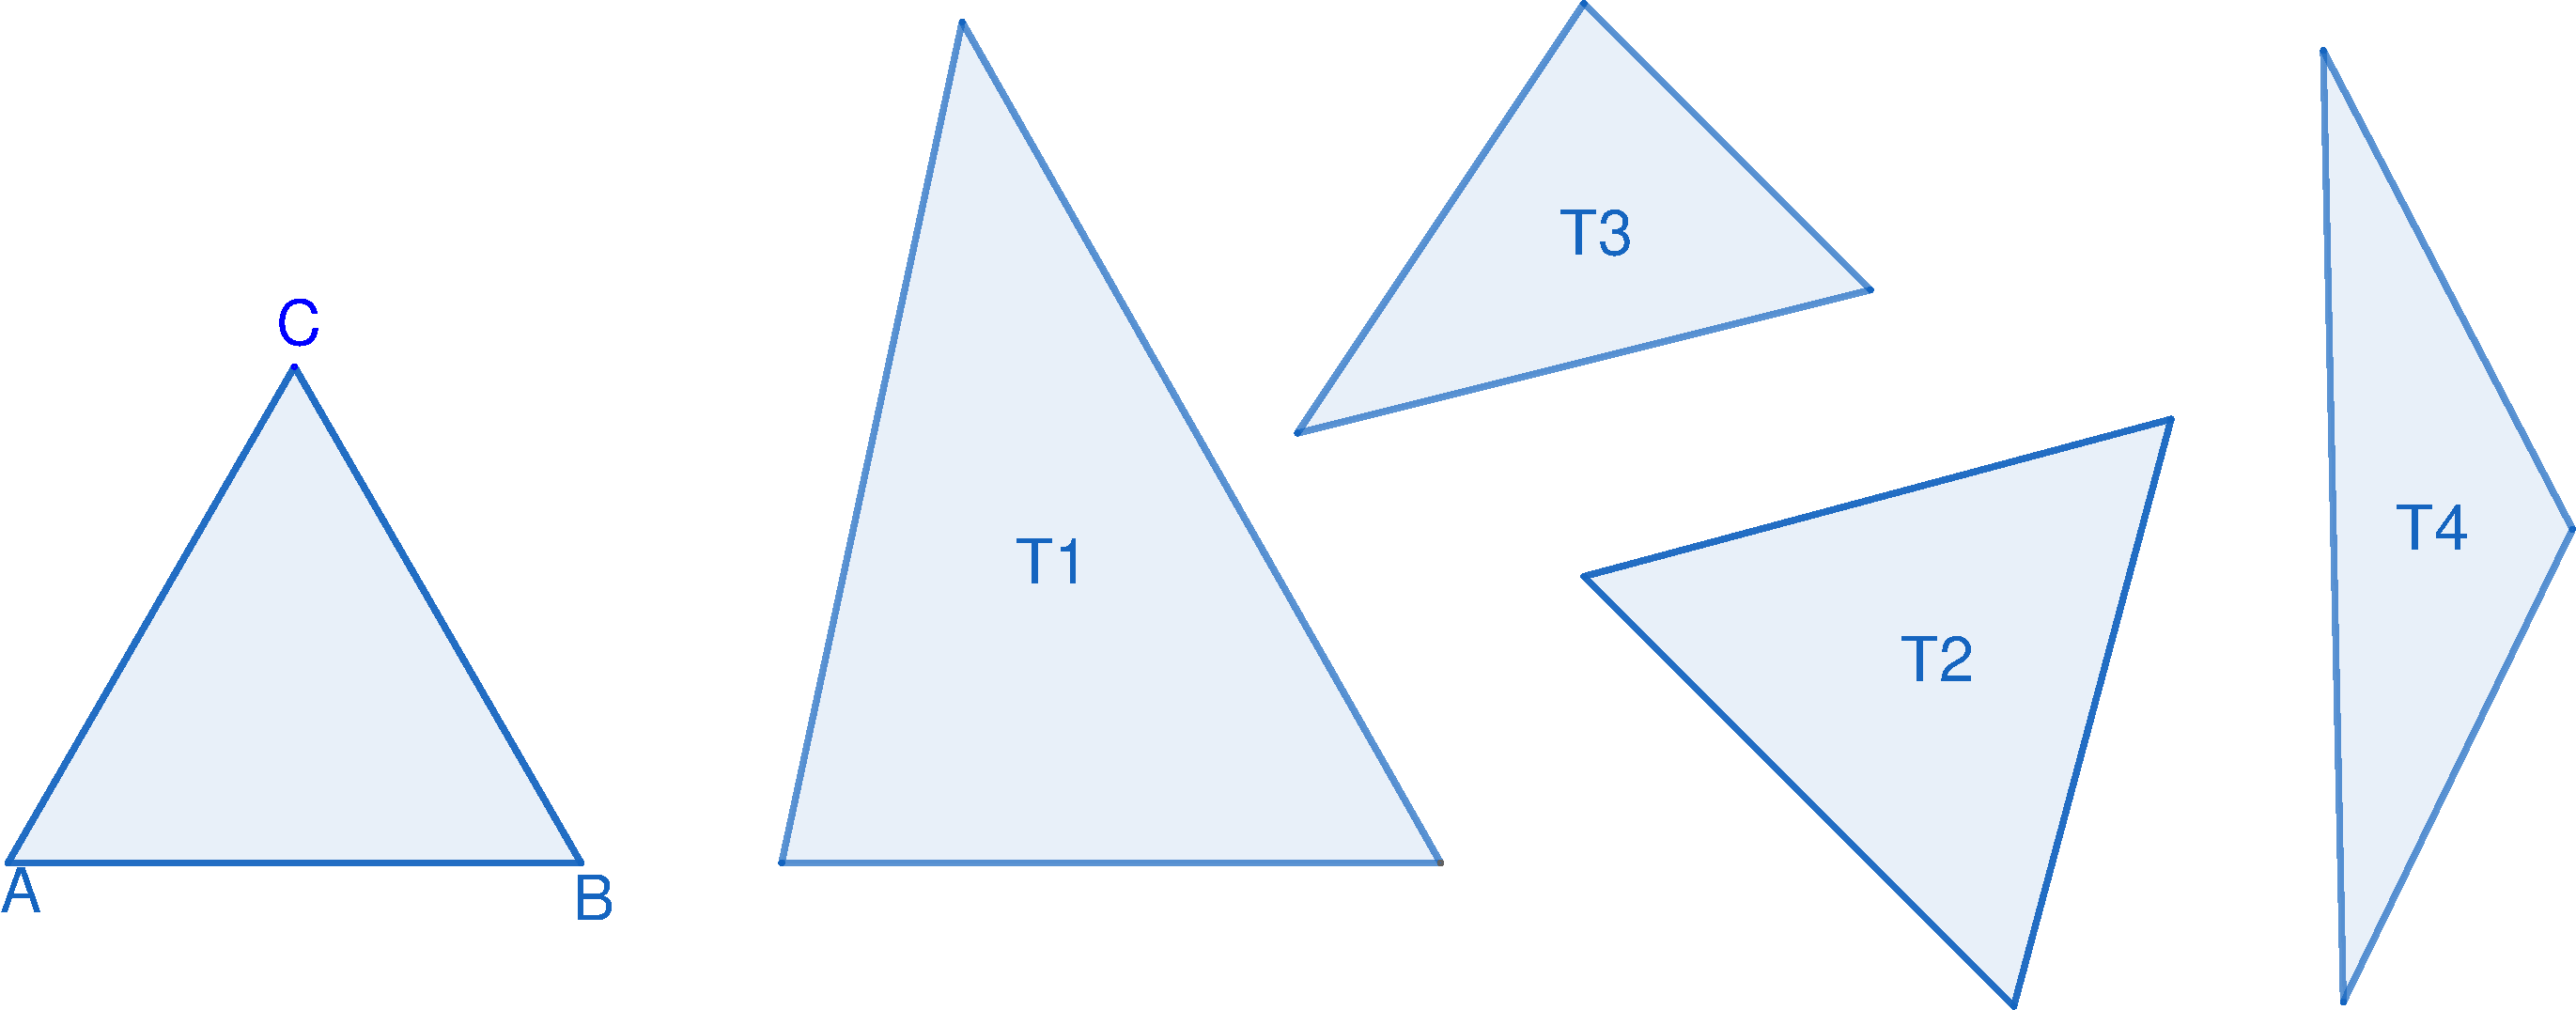
\includegraphics[width=5in]{images/dilation01}\end{center}
    \wbnewpage
    \item Rectangles R1, R2, R3, and R4 are all dilations of rectangle $ABCD$. Which one is a dilation with scale factor $\displaystyle\frac12$?\par
    \begin{center}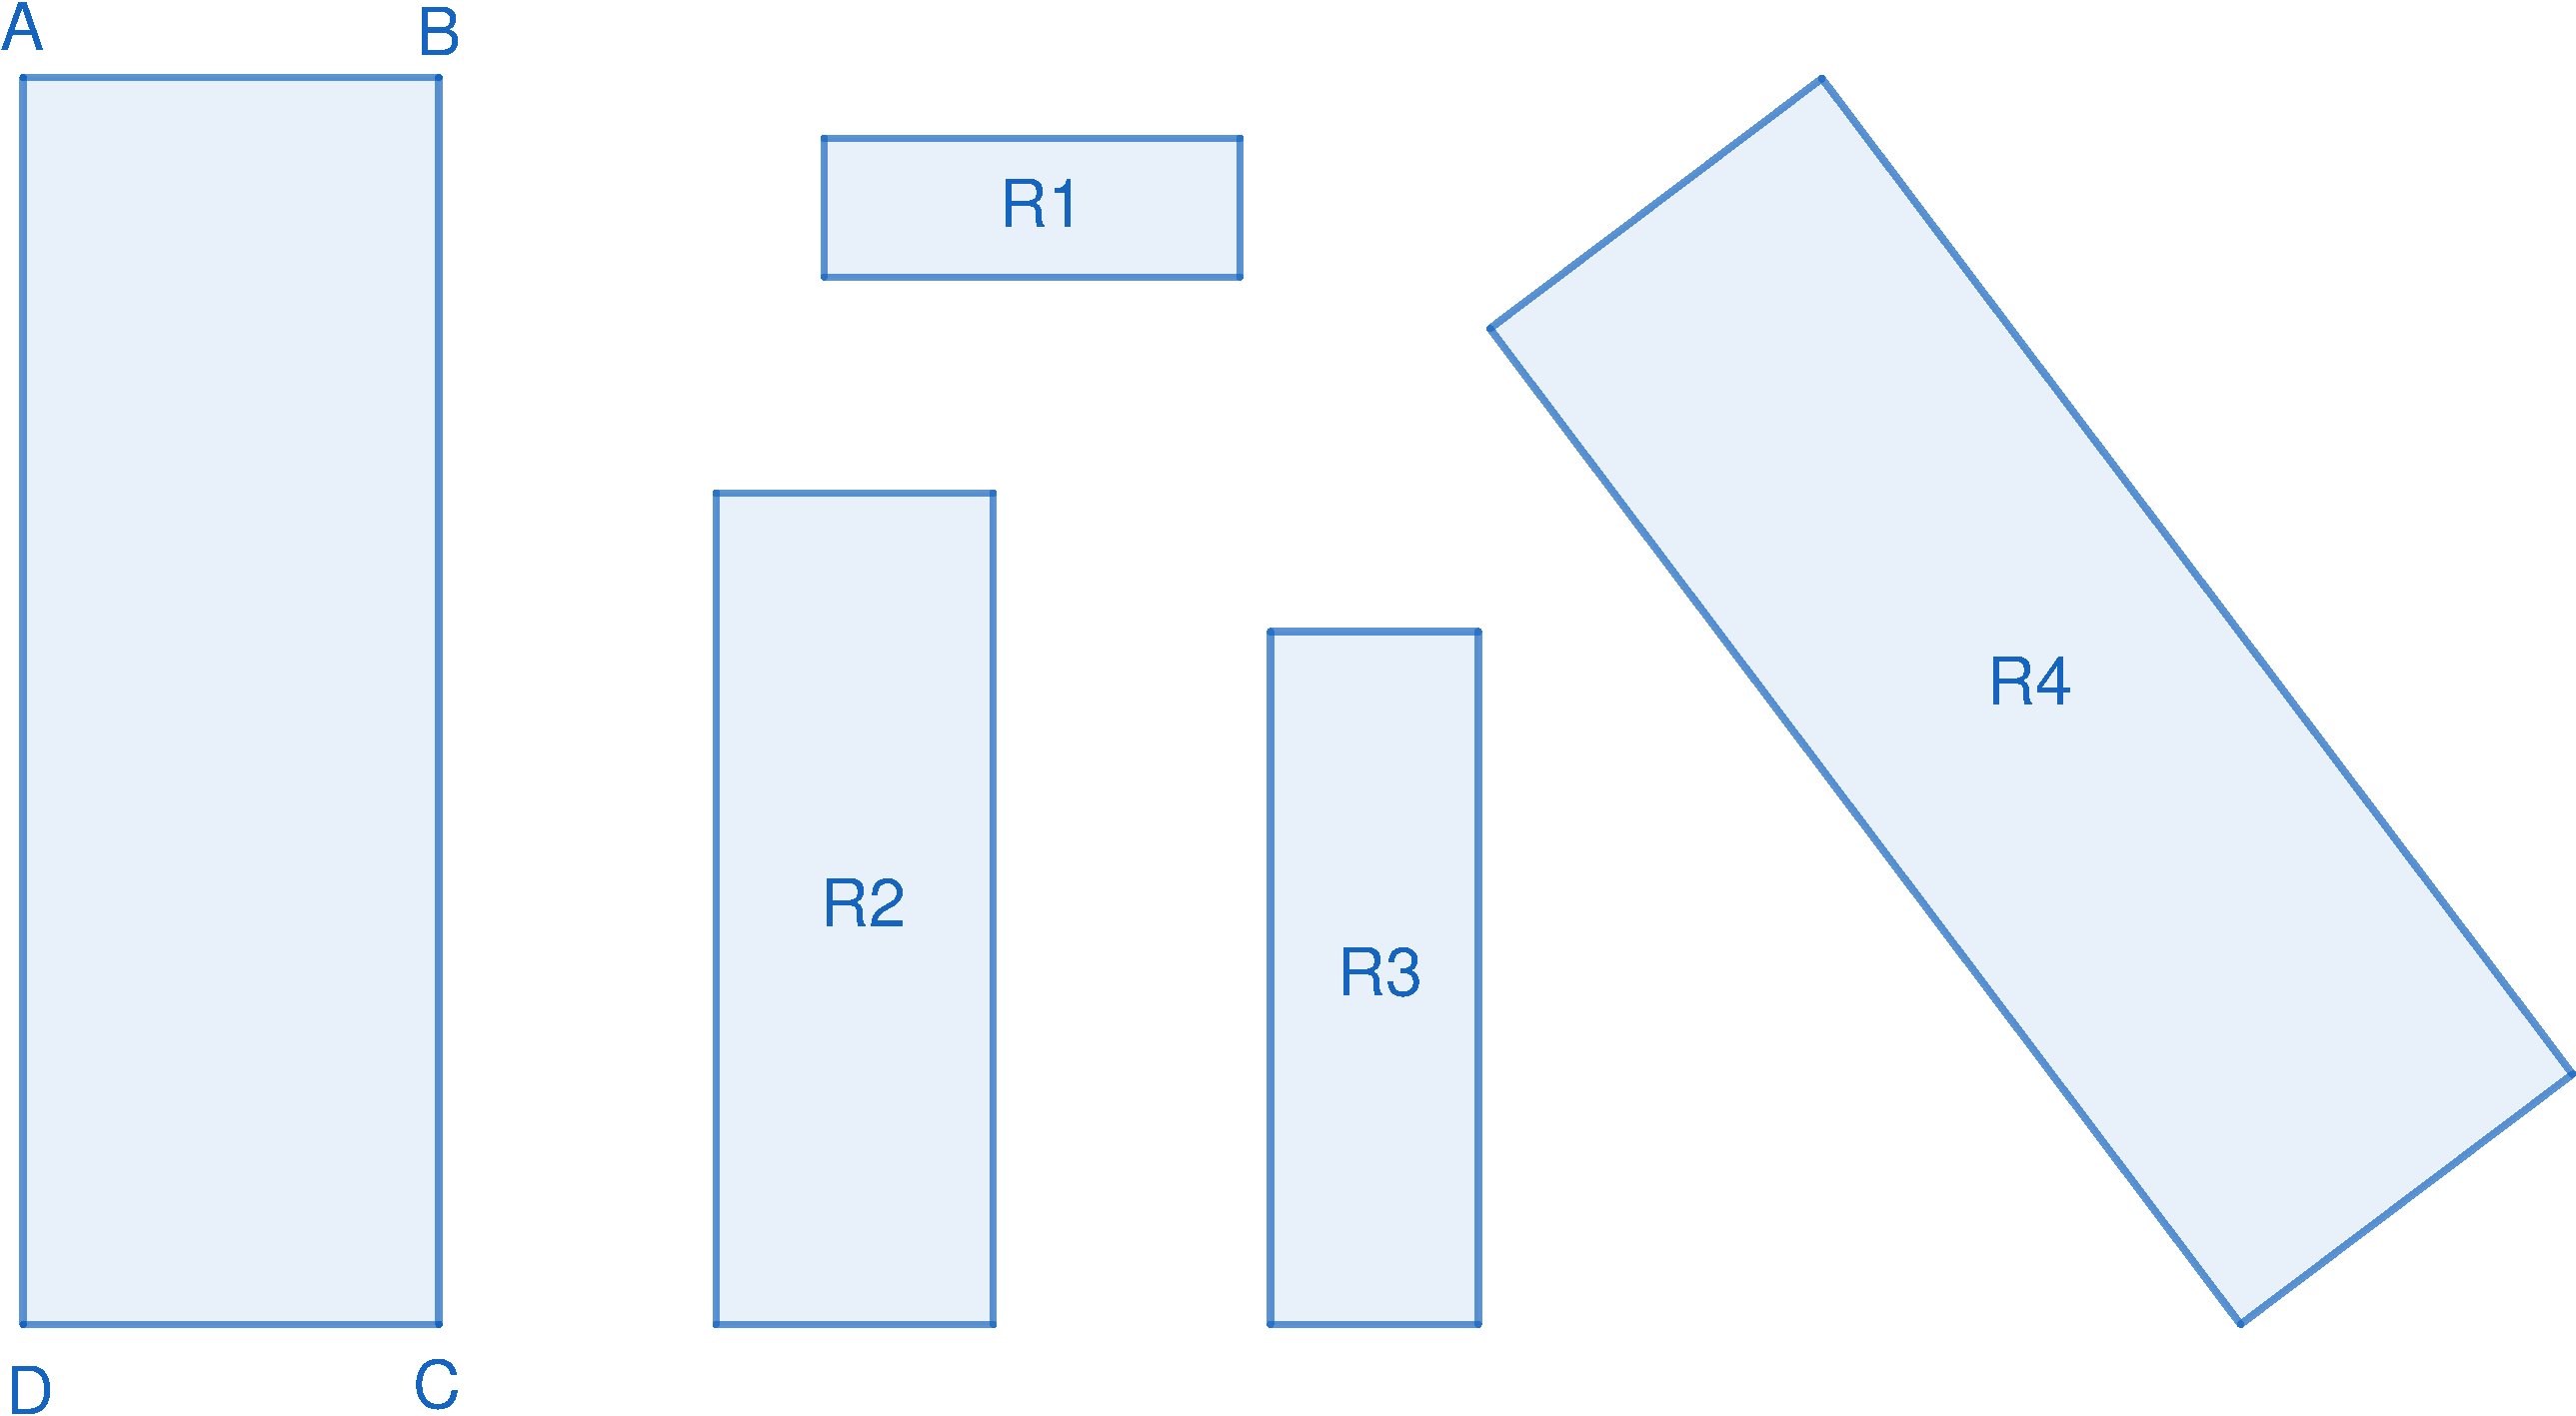
\includegraphics[width=5in]{images/dilation02}\end{center}
    \item Draw two separate dilations of hexagon $ABCDEF$---one with scale factor $\displaystyle \frac12$ and the other with scale factor $\displaystyle\frac23$.\par
    \begin{center}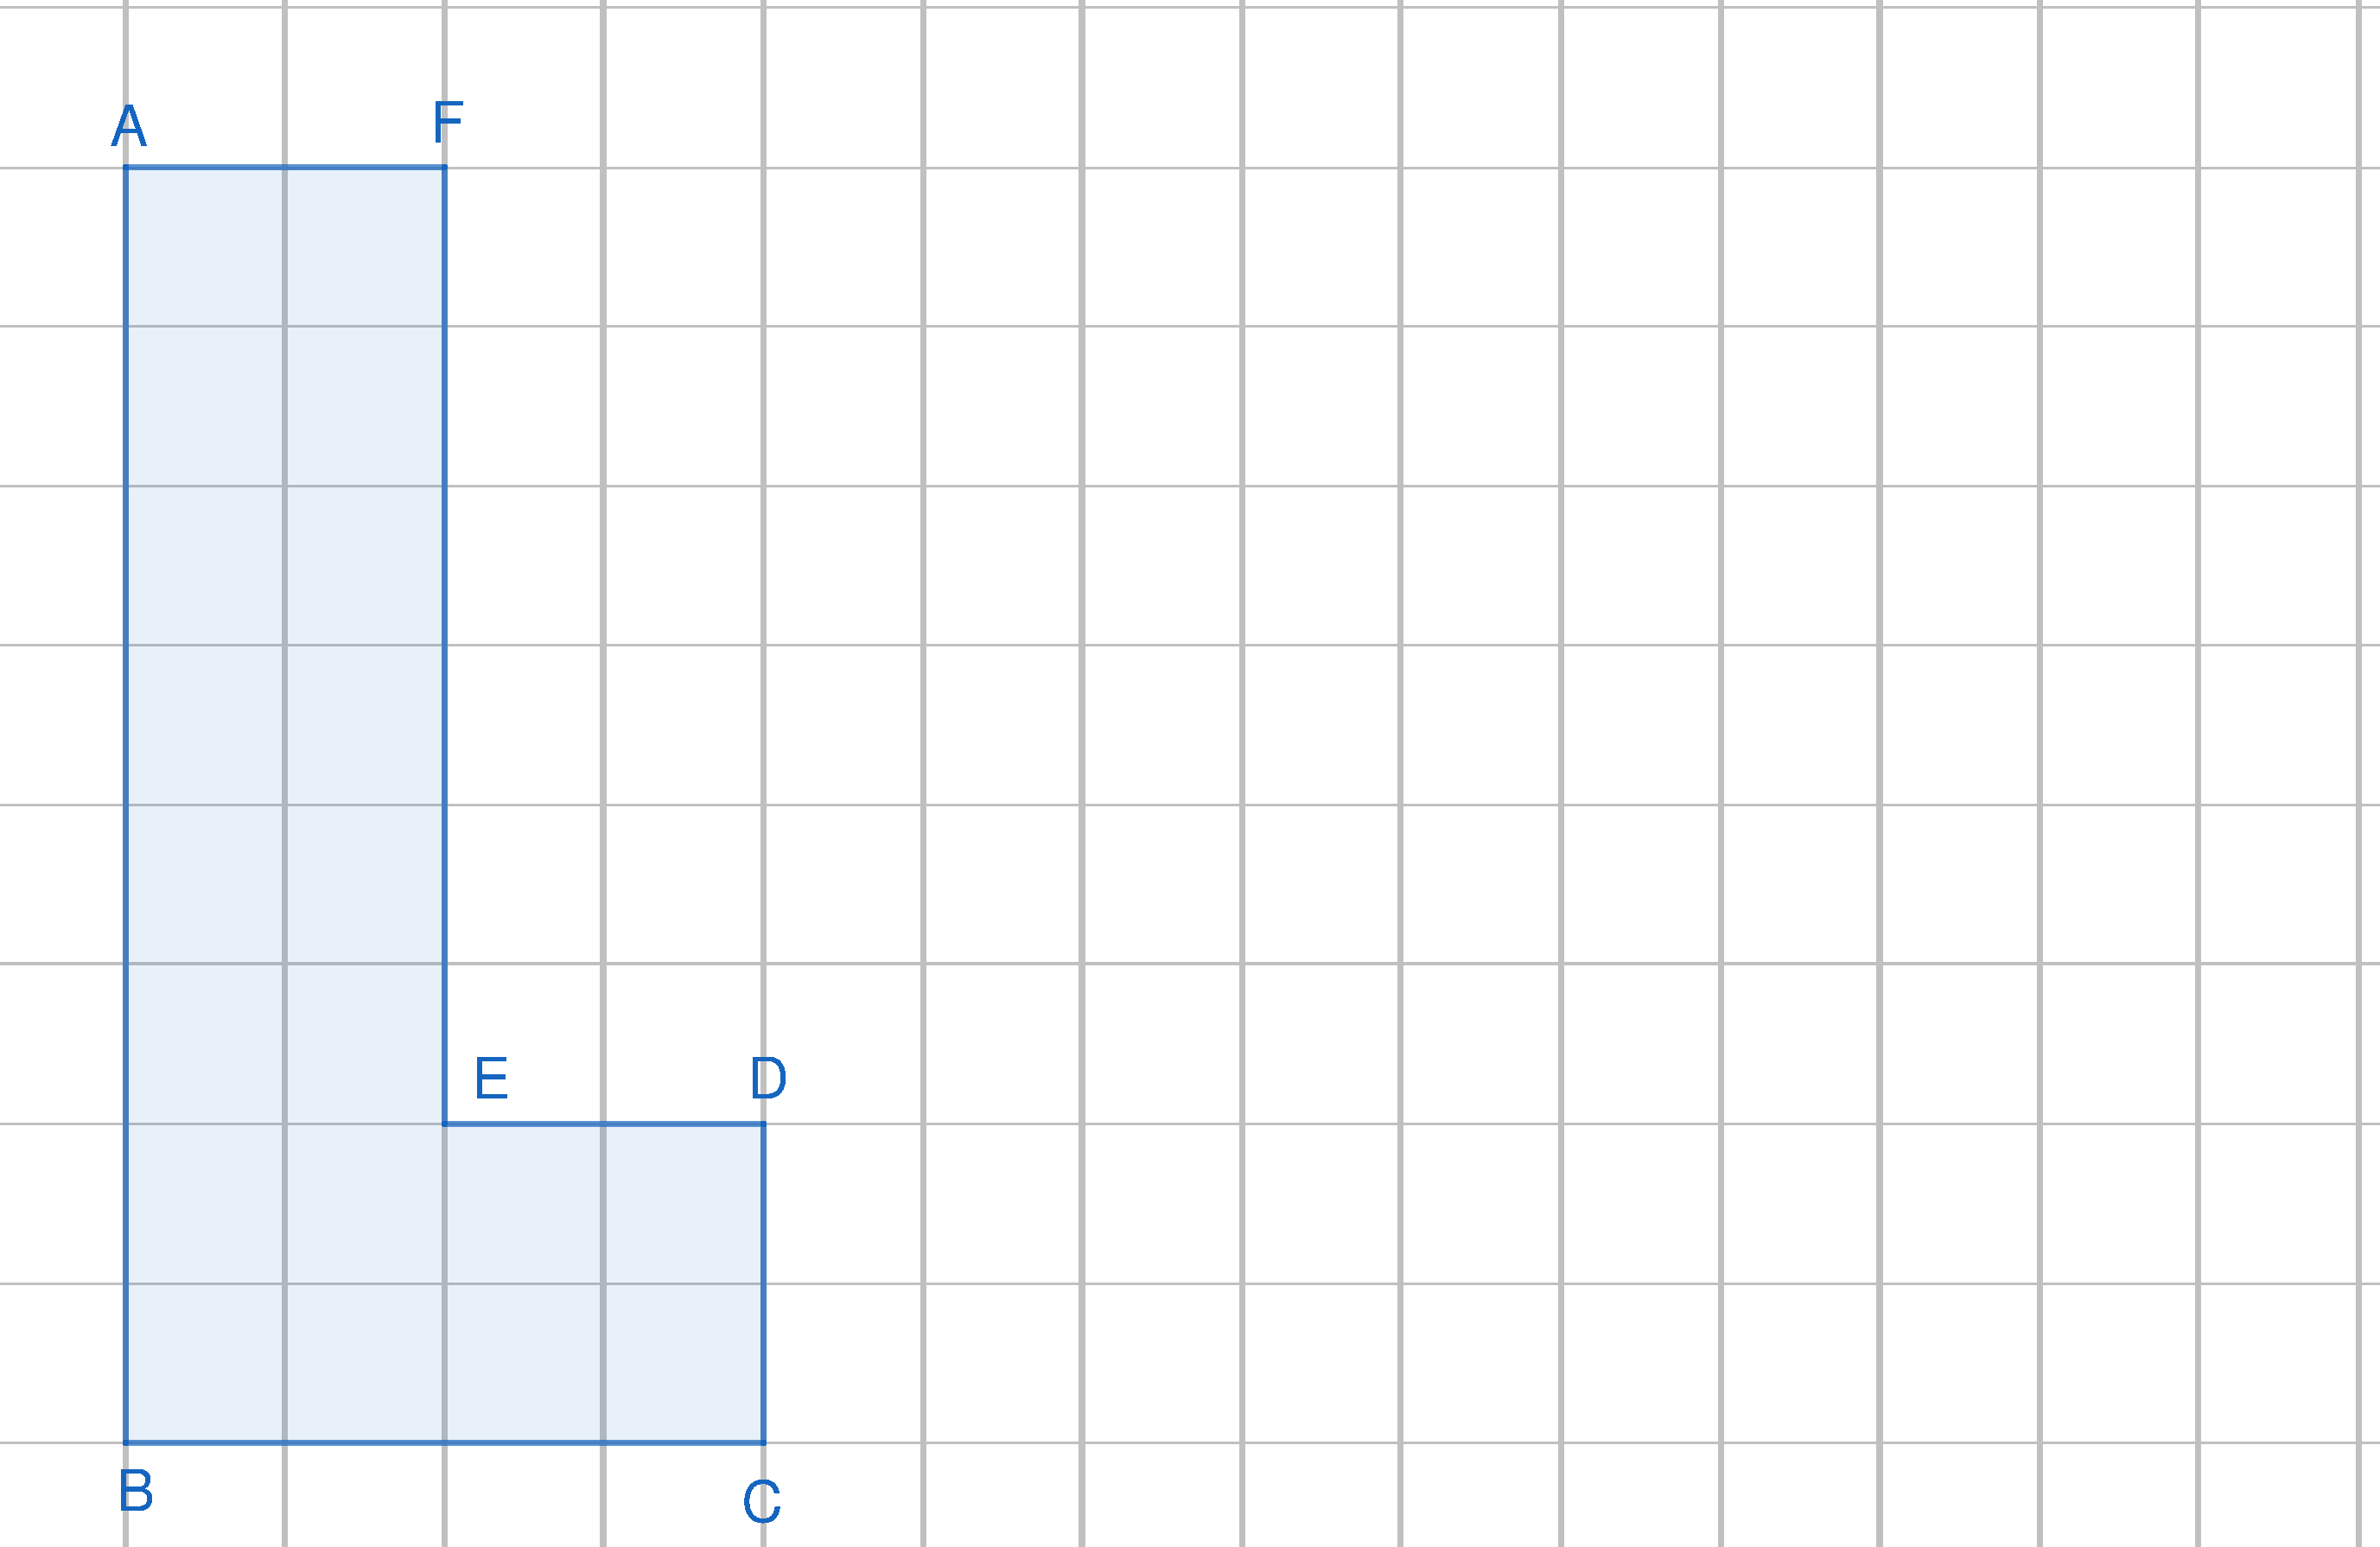
\includegraphics[width=5in]{images/dilation03}\end{center}
    \wbnewpage
    \item A circle with radius 4 is dilated with scale factor 3.
        \begin{enumerate}
            \item What is the radius of its image?\wbvfill
            \item What is the area of its image?\wbvfill
            \item What is the ratio of the area of the image to the area of the preimage? Careful! It is not 3:1.\wbvfill
        \end{enumerate}
    \item A cube with side length 2 cm is dilated with scale factor 10. What is the ratio of the volume of the image to the volume of the preimage?\wbvfill
\end{enumerate}

\wbnewpage
\subsection{Activity: Marble Weight Using Dilation}
A typical shooter marble has a 5/8 inch diameter (source  \href{https://www.marblecollecting.com/marble-reference/how-to-size-marbles/}{MarbleCollecting.com}),
\begin{center}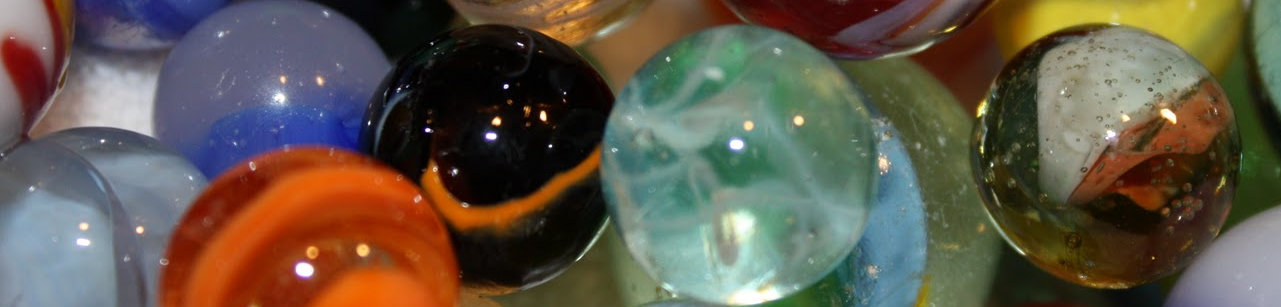
\includegraphics[width=4in]{images/marbles}\end{center}
weighs about 5.4 grams, and has about the same density as the humongous marble. We will use this information to calculate the weight of the humongous marble from the odditorium (see \ref{subsec:Odditorium})!
\begin{enumerate}
    \item Make sure you understand the problem.
    \item The plan for solving the problem comprises parts \ref{marble-first-step}-\ref{marble-last-step}. You will carry out that plan by answering those questions.
    \item \label{marble-first-step}Convert the weight of the shooter marble (5.4 grams) into pounds. Recall $1\text{ pound}=453.6\text{ grams}$.\wbvfill
    \item Estimate the diameter of the humongous marble in inches.\wbvfill
    \item Since a typical shooter marble is a sphere and the humongous marble is also a sphere, the humongous marble is a dilation of the tiny shooter marble. What is the scale factor?\wbvfill
    \wbnewpage
    \item \label{marble-ratio}What is the ratio of the volume of the humongous marble to the volume of the shooter marble?\wbvfill
    \item \label{marble-last-step}The ratio of the weight of the humongous marble to the weight of the shooter marble is the same as the ratio in part \ref{marble-ratio} (because weight and volume are proportional). Use this information to calculate the weight of the humongous marble.\wbvfill
    \item Review (problem solving step 4): Did this calculation give a weight similar to that from the calculation using density? Do the calculated weights seem reasonable? How do they compare to your initial guess? If you note any discrepancies or problems, where did the calculation(s) go wrong? See if you can spot the error(s) in this calculation or the calculation based on density.
    \wbvfill
\end{enumerate}
\Instr{ The sign in the background of this \href{https://upload.wikimedia.org/wikipedia/commons/5/5b/5-ton_floating_granite_ball.jpg}{wikimedia photo} gives the weight. It is 10,518 pounds. The marble is in front of the Ripley's Believe it or Not! odditorium in Gatlinburg, TN. You and your students can visit it in real life!}

\wbnewpage
\subsection{Activity: How tall is Engleman Hall?}
When the sun casts shadows onto level ground the triangle formed by a vertical object, its shadow, and the imaginary line from the top of the object to the tip of the shadow is similar to any other. This fact allows us to calculate the height of tall objects without the dangers of climbing them or unrolling a tape measure from their top to bottom.
\begin{enumerate}
    \item Draw a schematic diagram of an object, its shadow, and the imaginary line from the top of the object to the tip of its shadow. You may include a schematic of the sun, the ground, and anything else that you find helpful.\wbvfill\wbvfill
    \item Go outside and measure 
    \begin{enumerate}
        \item Your height\medskip
        \item The length of your shadow\medskip
    \end{enumerate}
    \item Find 3 tall objects whose heights you would like to calculate. Pick objects where their shadow, such as that of Engleman Hall, other building, tree, lamppost, flagpole, sculpture, etc. is cast on level ground where you can measure it. Write down the objects, their shadow lengths, and make a guess as to how tall each one is. Record your measurements and your guesses here. Then return to your classroom.
    \par\smallskip\noindent\setlength{\extrarowheight}{15pt}
    \begin{tabular}{|>{\raggedright}p{2in}|>{\raggedright}p{1.5in}|>{\raggedright}p{1.5in}|}
        \hline 
            Object & Shadow length & Guess of height\tabularnewline
        \hline 
            &  & \tabularnewline
        \hline 
            &  & \tabularnewline
        \hline 
            &  & \tabularnewline
        \hline 
    \end{tabular}
    \setlength{\extrarowheight}{0pt}
    \wbnewpage
    \item Use the fact that all triangles defined by a vertical object, its shadow, and the imaginary line from the top of the object to the tip of its shadow are dilations of one another to calculate the height of Engleman Hall (or other object whose shadow you measured).
\end{enumerate}
\Instr{  Students may remember studying similar triangles in geometry, but they need not refer to any of that to succeed with this problem. They should realize that the triangle formed by the tall object and its shadow is a dilation of the triangle formed by their body and its shadow. The scale factor between their body's shadow and the objects shadow should be used to scale their height up to the height of the tall object.}

\wbnewpage
\subsection{Entrance Activity: Sharpie!}
When we say that two things are similar in English, we mean that they resemble one another in some way, but are not exactly the same. Just how closely they resemble one another and in what way is entirely up to the speaker. However, when we say two things are similar in mathematics, we mean they are the exact same shape but perhaps different sizes. The way in which they resemble one another is precisely defined. In terms of ratios, two objects are similar if corresponding lengths between the two objects maintain a constant ratio.

Say you have two photos of the same clown, one is a 4x6 and the other 8x10. In the 4x6 photo, the distance between the clown's pupils is one inch and in the 8x10 photo, the distance between the clown's pupils in 2 inches. If the two photos are similar in the mathematical sense, then all corresponding distances between the two photos will have a 2:1 ratio. Say the distance from the center of his big red nose to the furthest point on his big right ear is 1.3 inches on the 4x6 photo. Then the distance from the center of his big red nose to the furthest point on his big right ear on the 8x10 photo must be 2.6 inches. The conversion factor from distance on the 4x6 photo to distance of the 8x10 photo is 2. If this ratio holds for all distances in the photo, then the photos (clowns) are similar in the mathematical sense. However, if there is even one distance (say the width of the clown's nose) for which this ratio does not hold (perhaps it is 1/3 inches in the 4x6 and only 1/2 inches in the 8x10), then the photos are not similar. In the language of the previous sections, we would say the width of the clown's nose is out of proportion or the 8x10 photo is not a dilation of the 4x6 photo. For two shapes to be similar all of their features must be in proportion. They must be dilations of one another.

\Instr{  You may need to hold a discussion about the following photo. Make sure everyone understands the difference between the word similar in the English sense and in the mathematical sense. The markers are clearly similar in the English sense--both markers, black top with pocket clip, gray body, rounded ends, etc. However, they are just as clearly NOT similar in the mathematical sense. They are just about the same length--the large one is about 10\% longer (ratio of lengths 1.1:1 or so). Cap lengths seem to be in about the same ratio. Body (gray) lengths also share the same ratio. But their widths do not share the same ratio at all. The big one is about 50\% wider (ratio of widths 1.5:1 or so). In any case, the ratio between their lengths and the ratio between their widths are clearly not equal. Students may be given copies of the photo and rulers to make some measurements. You may also wish to have a yard stick handy and have students measure the image on the classroom screen. You may want to steer them away from discussing differences in the markings as proof that they are not similar in the mathematical sense. There are no obvious corresponding distances to compare within the markings.}
\begin{center}
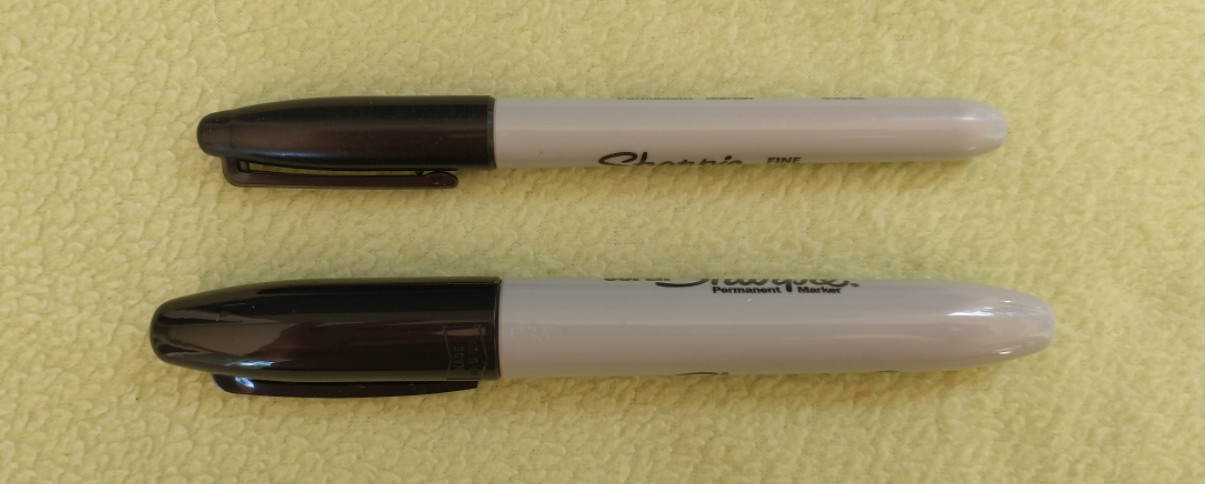
\includegraphics[width=5.5in]{images/similarMarkers}
\par\end{center}
\begin{enumerate}
\item Are the markers similar in the English sense?\wbvfill
\item Are the markers similar in the mathematical sense?\wbvfill
\end{enumerate}

\wbnewpage
\subsection{Entrance Activity: Self-similarity}
Watching movies is fun. Surfing the web is fun. Thumbing through a magazine is fun. Everywhere we look we see images. Behind each image is a great deal of mathematics. Some digital images are processed. They may have had their colors changed or their subjects touched up. Some digital images are compressed. They have been encoded to use less computer memory. To make storing, processing, compressing, and reproducing digital images happen a great deal of mathematics is used. One technique used is fractal image compression (see this \href{https://www.ijsr.net/archive/v5i7/ART2016513.pdf}{IJSR} article, for example). Can you tell which of these images are fractals and which are not?

\begin{center}
\begin{tabular}{ccc}
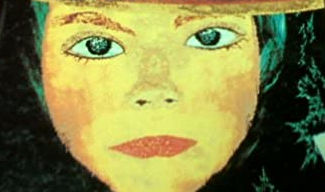
\includegraphics[height=1.4in]{images/fractalsEverywhere} & 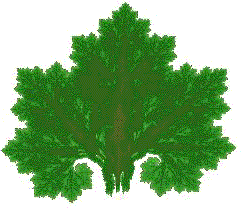
\includegraphics[height=1.4in]{images/MapleLeaf} & 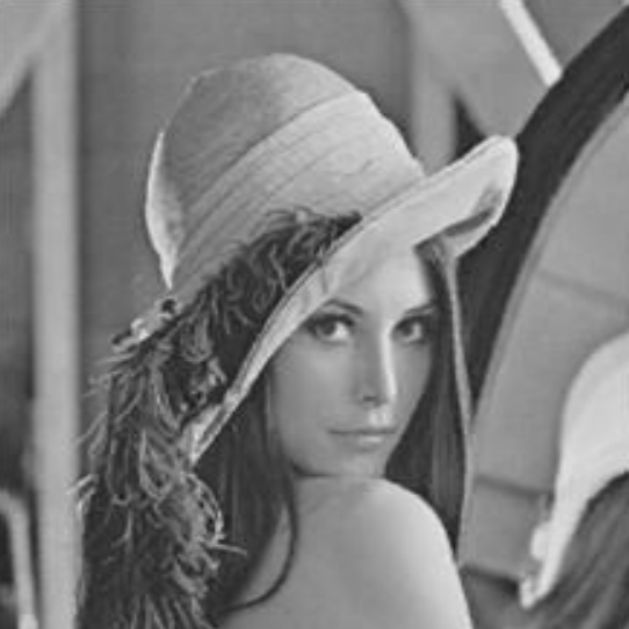
\includegraphics[height=1.4in]{images/LenaPhoto}\hfill \\
Artwork or fractal? & Maple leaf or fractal? & Photo or fractal?
\end{tabular}
\end{center}

They are all fractals! The basic idea behind all of these fractals is self-similarity. An object or shape is self-similar if parts of it look like the whole. Broccoli is a great example of a self-similar shape from nature.

\begin{center}
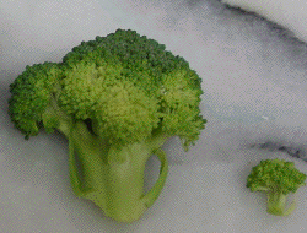
\includegraphics[height=1.5in]{images/broccoli}\hspace{.25in}
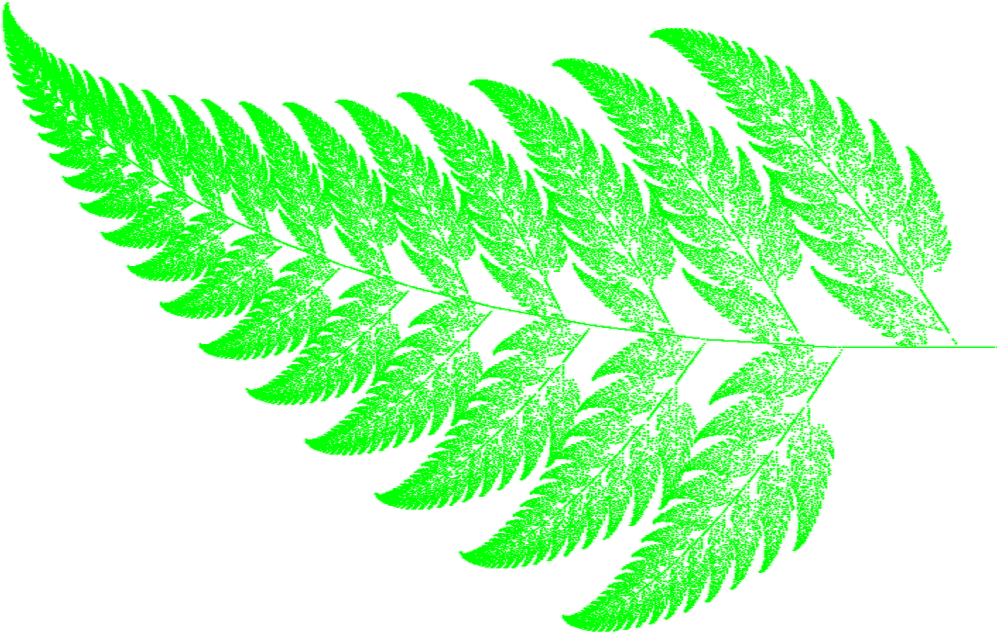
\includegraphics[height=1.5in]{images/fern}
\end{center}
The small piece of the broccoli head resembles the whole head! The fronds of the fern resemble the whole fern!

Which of the following natural shapes are self-similar (have parts that resemble the whole)? Circle them.

\begin{center}
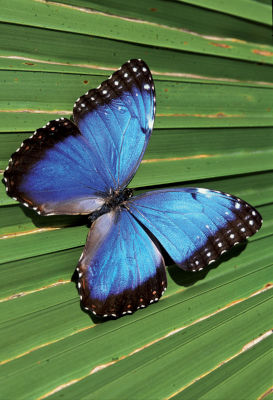
\includegraphics[height=1.5in]{images/butterfly}\hfill
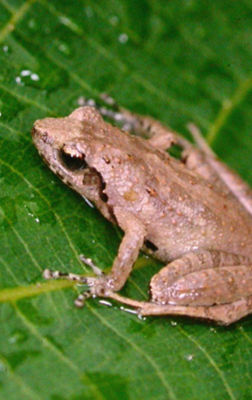
\includegraphics[height=1.5in]{images/frog}\hfill
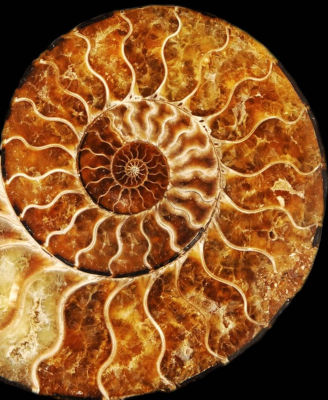
\includegraphics[height=1.5in]{images/nautilus}\hfill
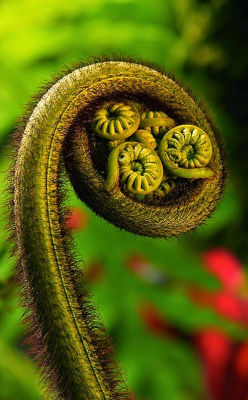
\includegraphics[height=1.5in]{images/spiralHead}\hfill
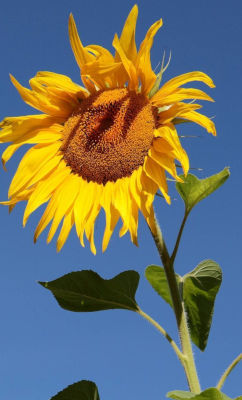
\includegraphics[height=1.5in]{images/sunflower}
\end{center}

\wbnewpage
\subsection{Activity: Rep-tiles}
Rep-tiles are perfectly self-similar shapes. A rep-tile can be replicated by fitting together copies of itself without overlap. For example, a square is a rep-tile because four congruent squares can be fitted together to form a square. There are other ways to fit squares together to form a square too! As seen below, five congruent squares plus a sixth square of double their size (dilation by a factor of 2) can be fitted together to form a square. Even though it may not be clear from the diagram, the rightmost image shows 31 squares of different sizes fitting together to form a square.
\begin{center}
    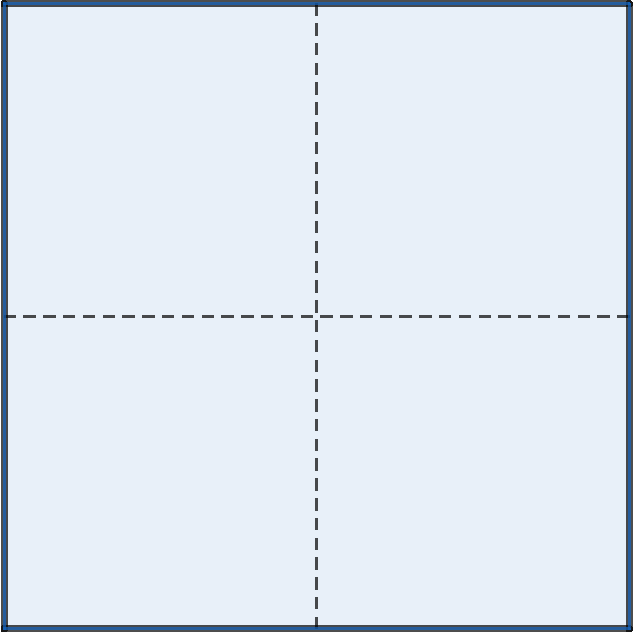
\includegraphics[height=1.8in]{images/rep-tile01} \hfill 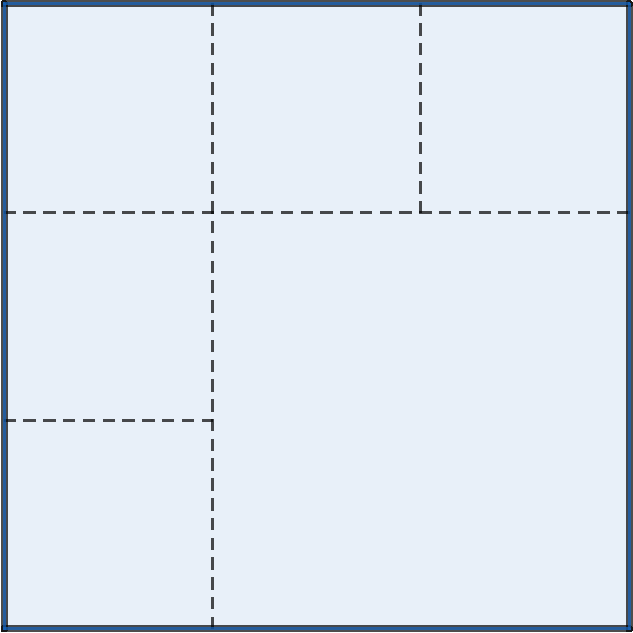
\includegraphics[height=1.8in]{images/rep-tile02} \hfill 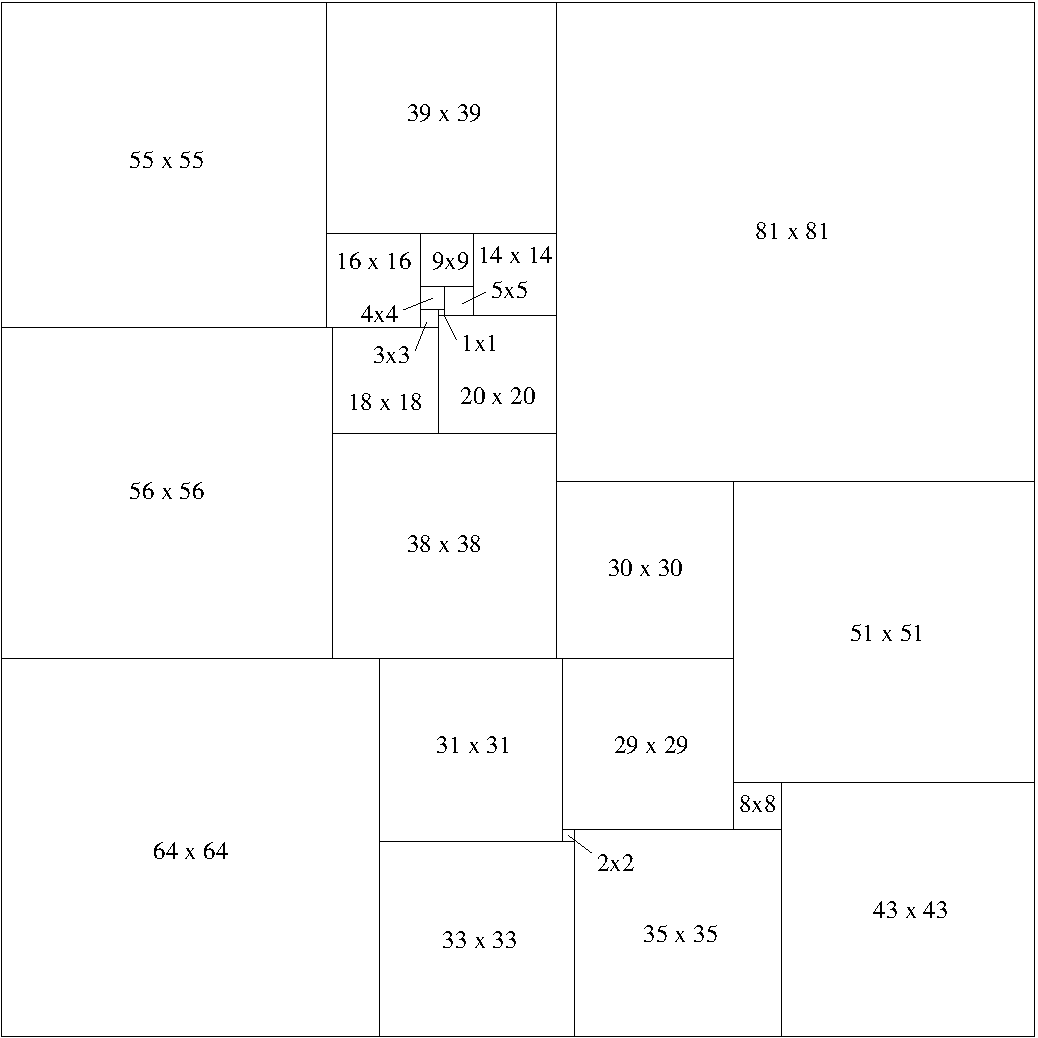
\includegraphics[height=1.8in]{images/gardner-01}
\end{center}
Can you fit four congruent copies of the following three rep-tiles together to create a replica of the whole? The rectangles must be put together to form a rectangle. The equilateral triangles must be put together to form an equilateral triangle. The L-shaped hexagons must be fitted together to form an L-shaped hexagon.
\begin{center}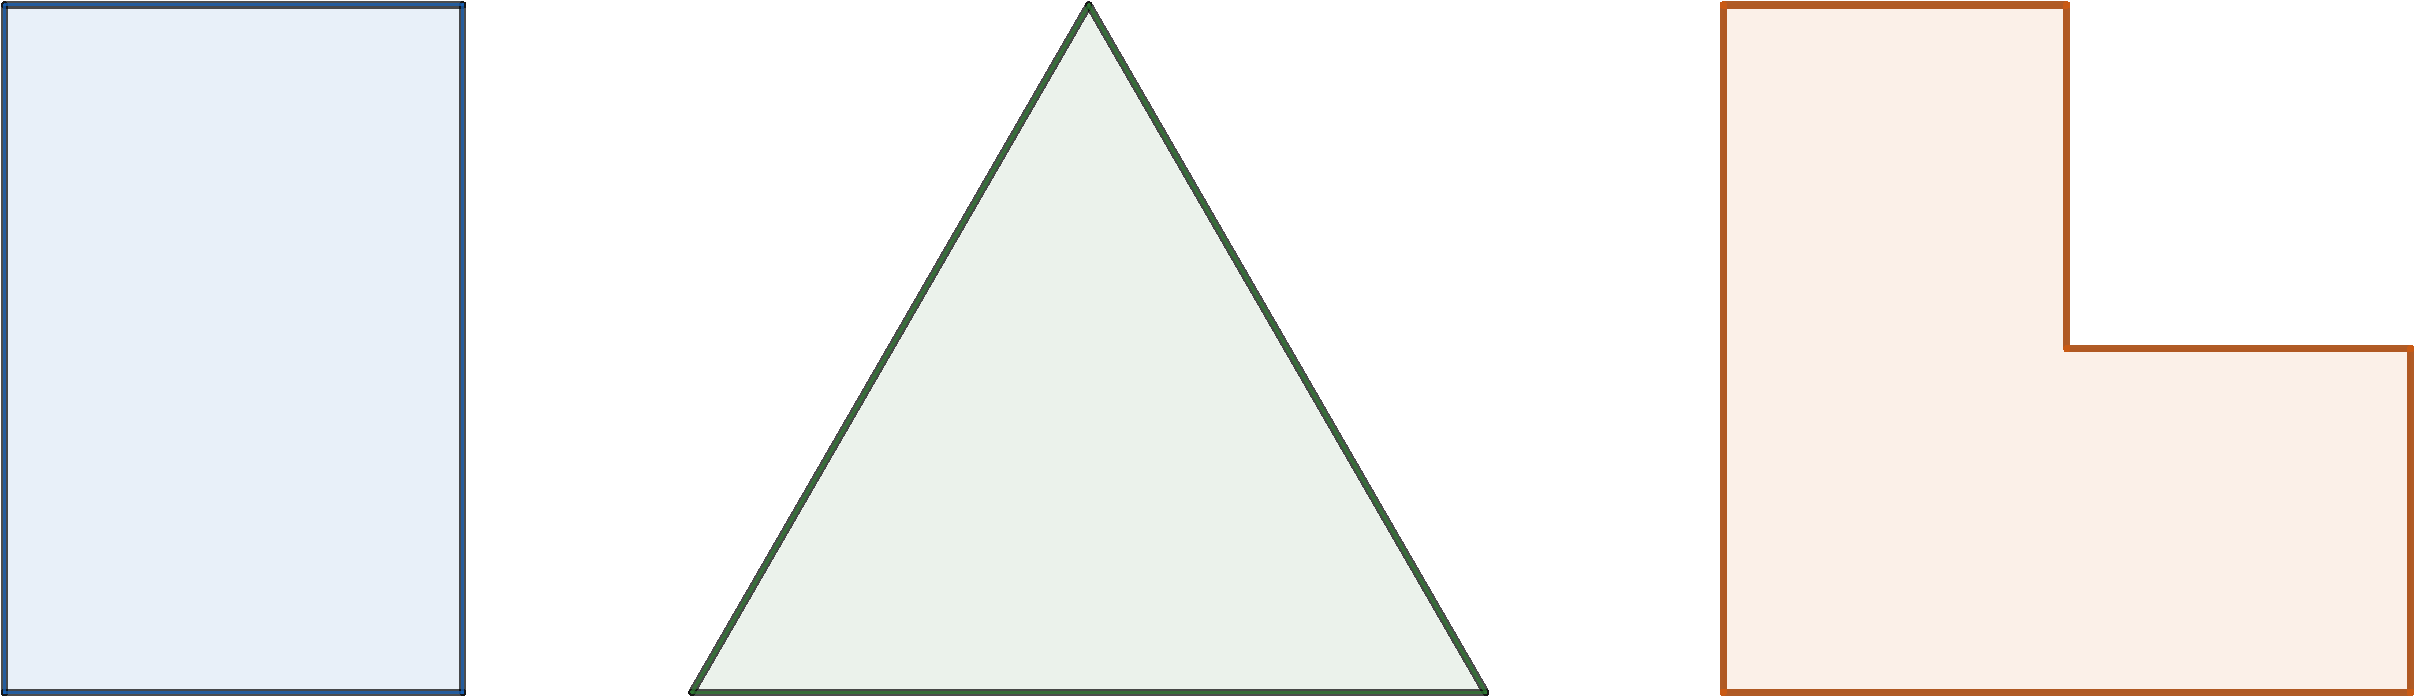
\includegraphics[height=1.7in]{images/rep-tile03}\end{center}
Cut out the copies below and see if you can fit them together on the shapes above.
\begin{center}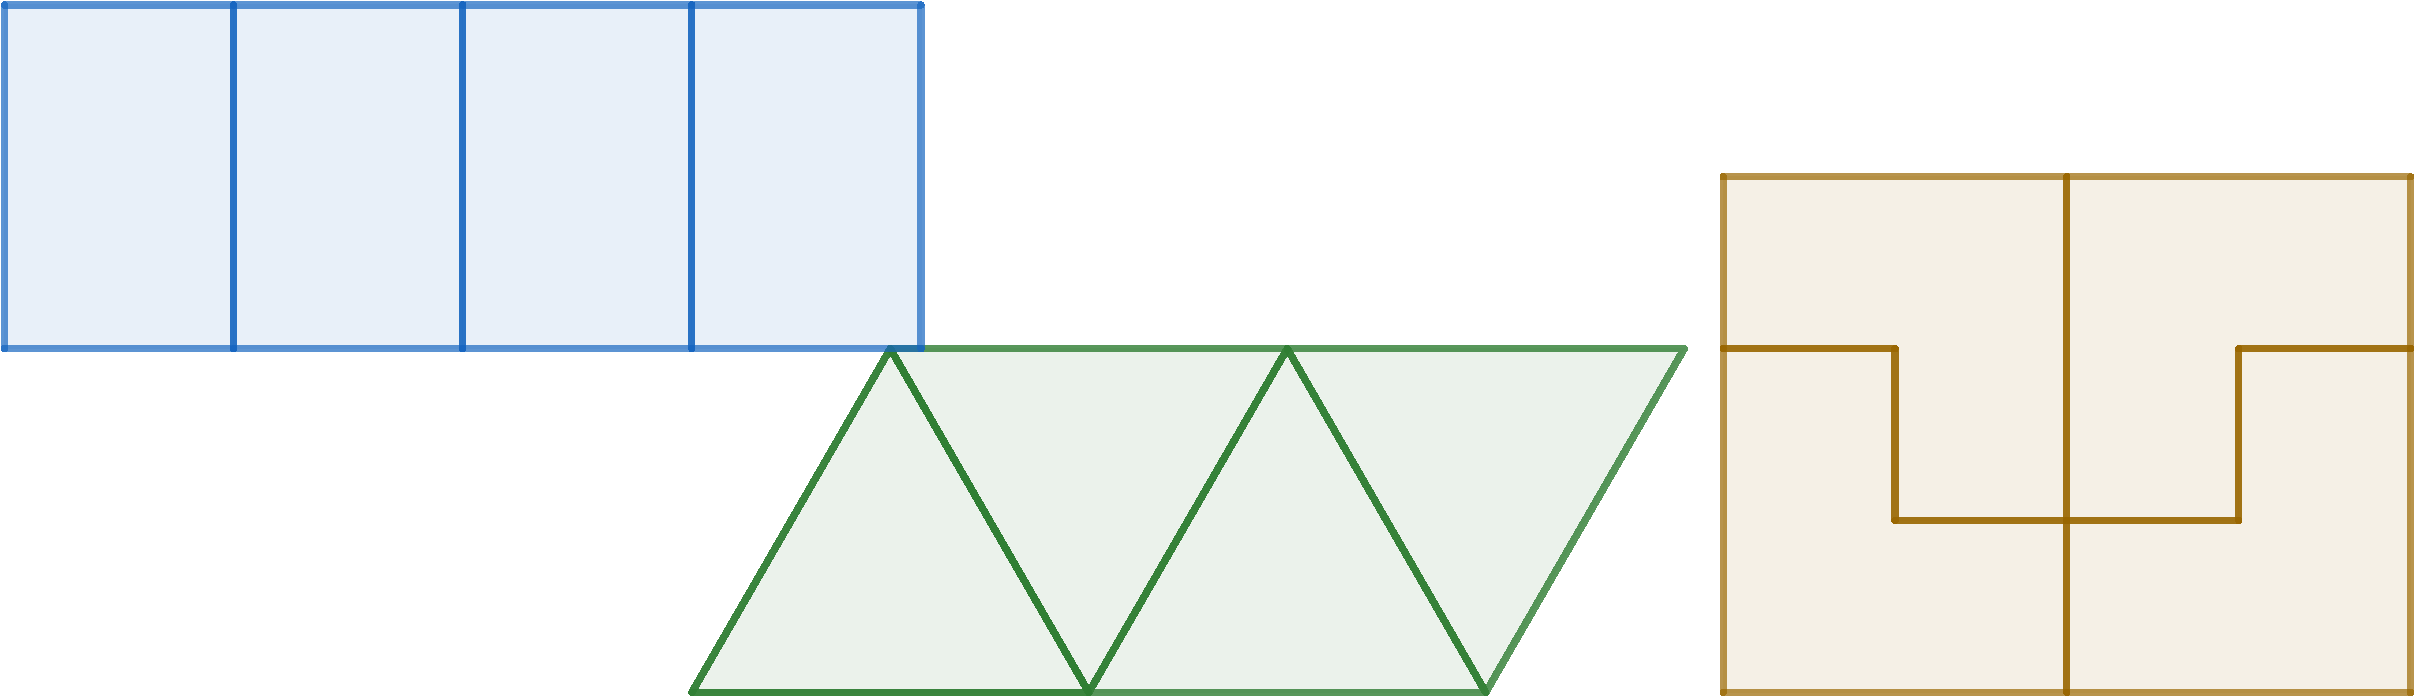
\includegraphics[height=1.7in]{images/rep-tile05}\end{center}
\Instr{ Here is one way to dissect each shape. There are many others!
\begin{center}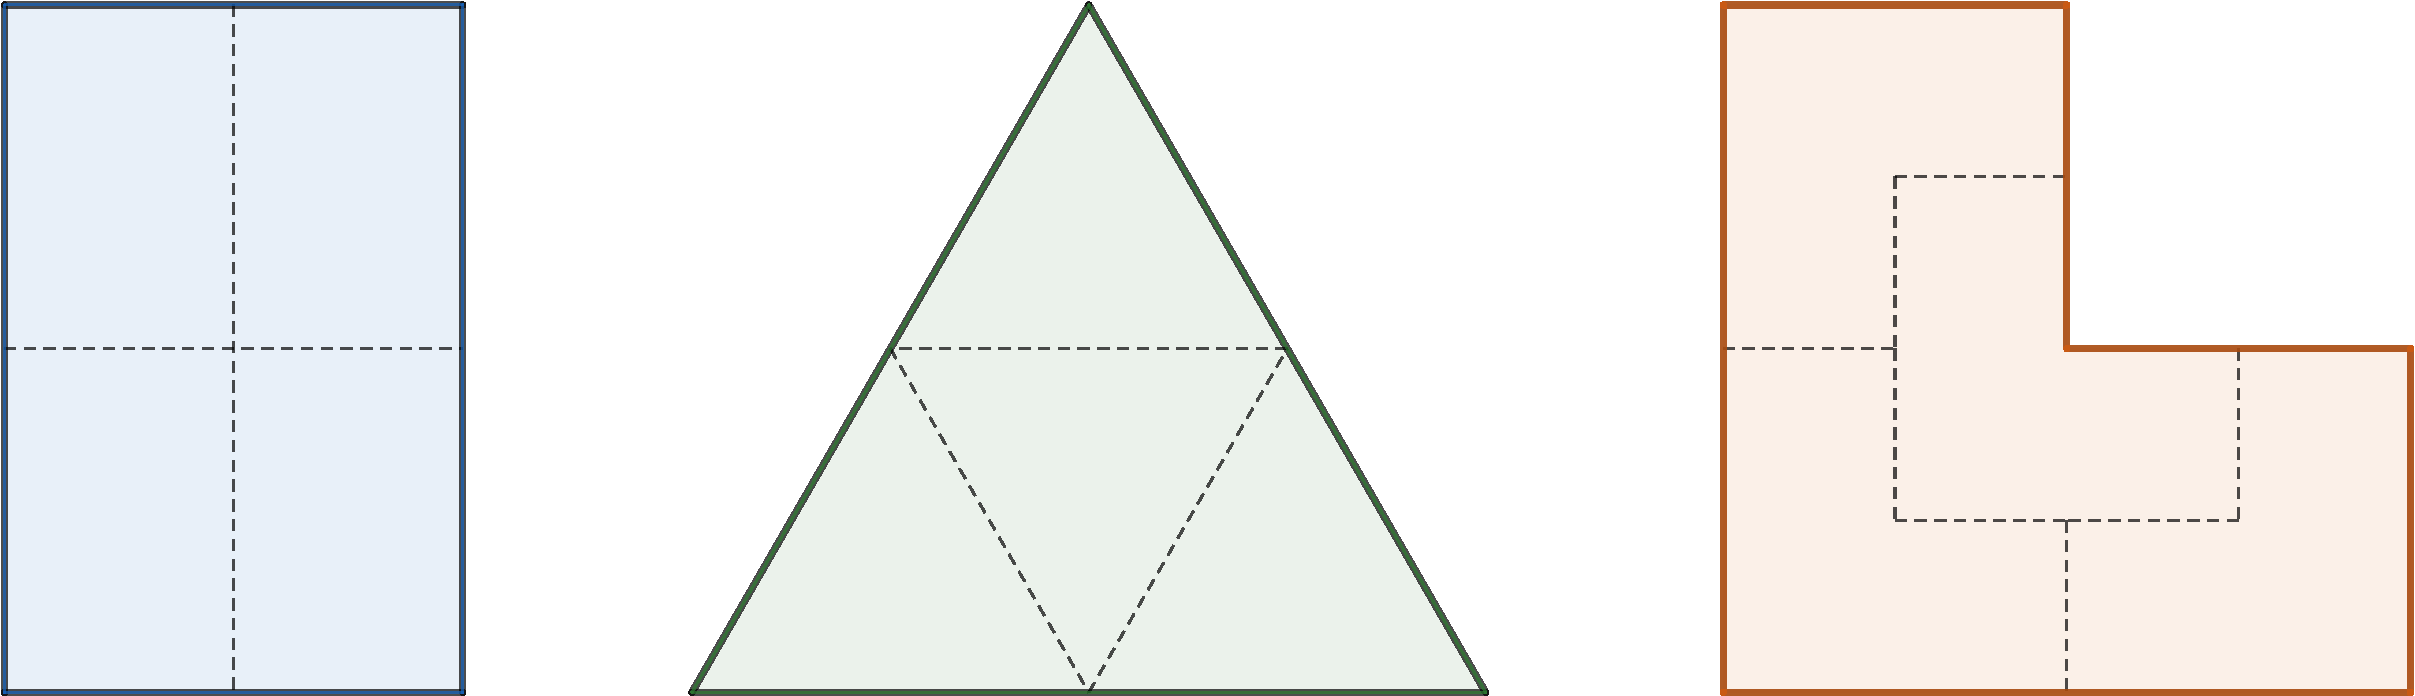
\includegraphics[height=1.7in]{images/rep-tile04}\end{center}}

\wbnewpage
\subsection{Activity: Similarity and Self-similarity}
\begin{enumerate}
\item Consider this photo of three pencils.
\begin{center}
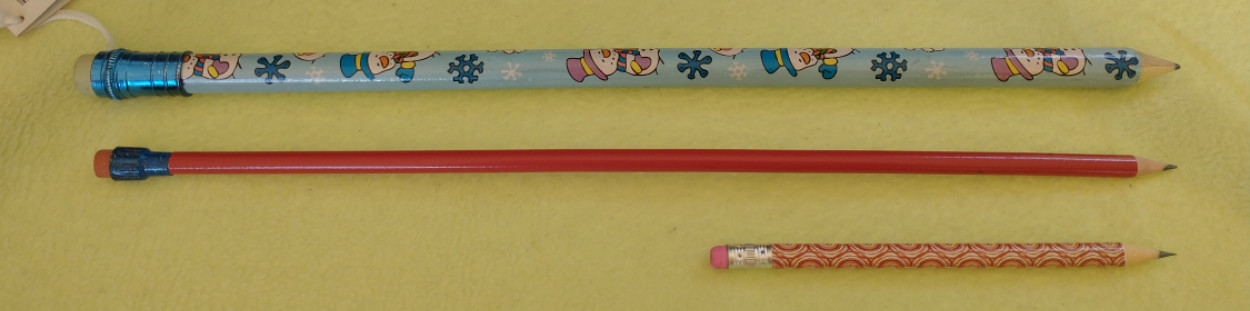
\includegraphics[width=5in]{images/similarPencils}
\par\end{center}
\begin{enumerate}
\item Are the pencils similar in the English sense?
\item Are the pencils similar in the mathematical sense? Consider only the
shapes, not the patterns printed on them.
\end{enumerate}
\Instr{  (a) Yes, they are similar in the English sense. They are all pencils, shaped with one dull end and one sharp end. (b) The top two are not similar in the mathematical sense. They have the same lengths but  different widths. Their length to length ratio is 1:1 while their width to width ratio is about 2:1 so they are not similar. The bottom two are not similar in the mathematical sense.}
\item Which illustrations are rep-tiles (perfectly self-similar shapes)? Circle them.
\begin{center}
    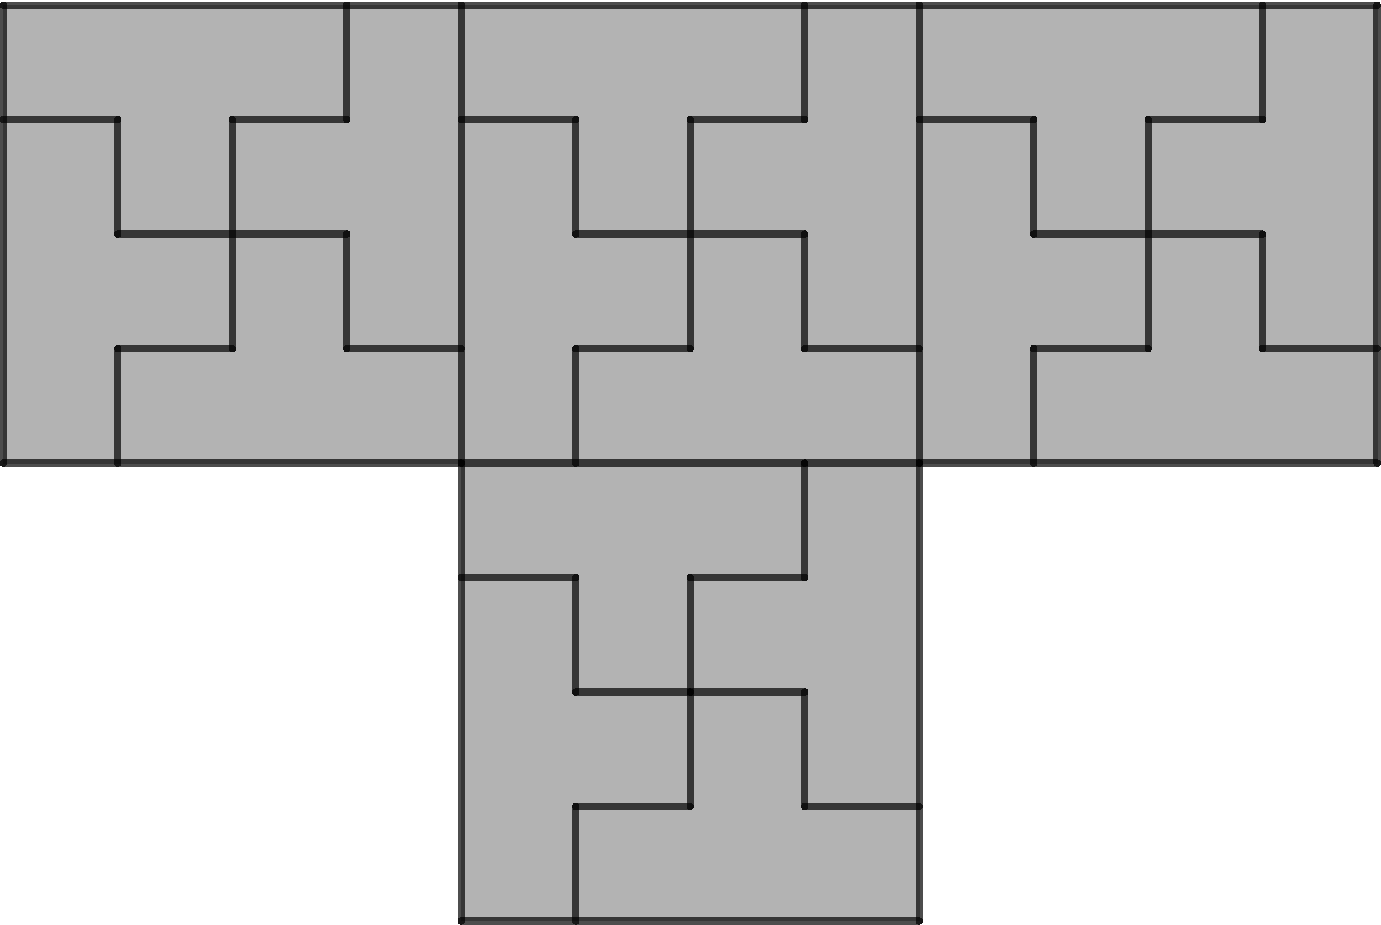
\includegraphics[height=1.6in]{images/rep-tile-72} \hfill
    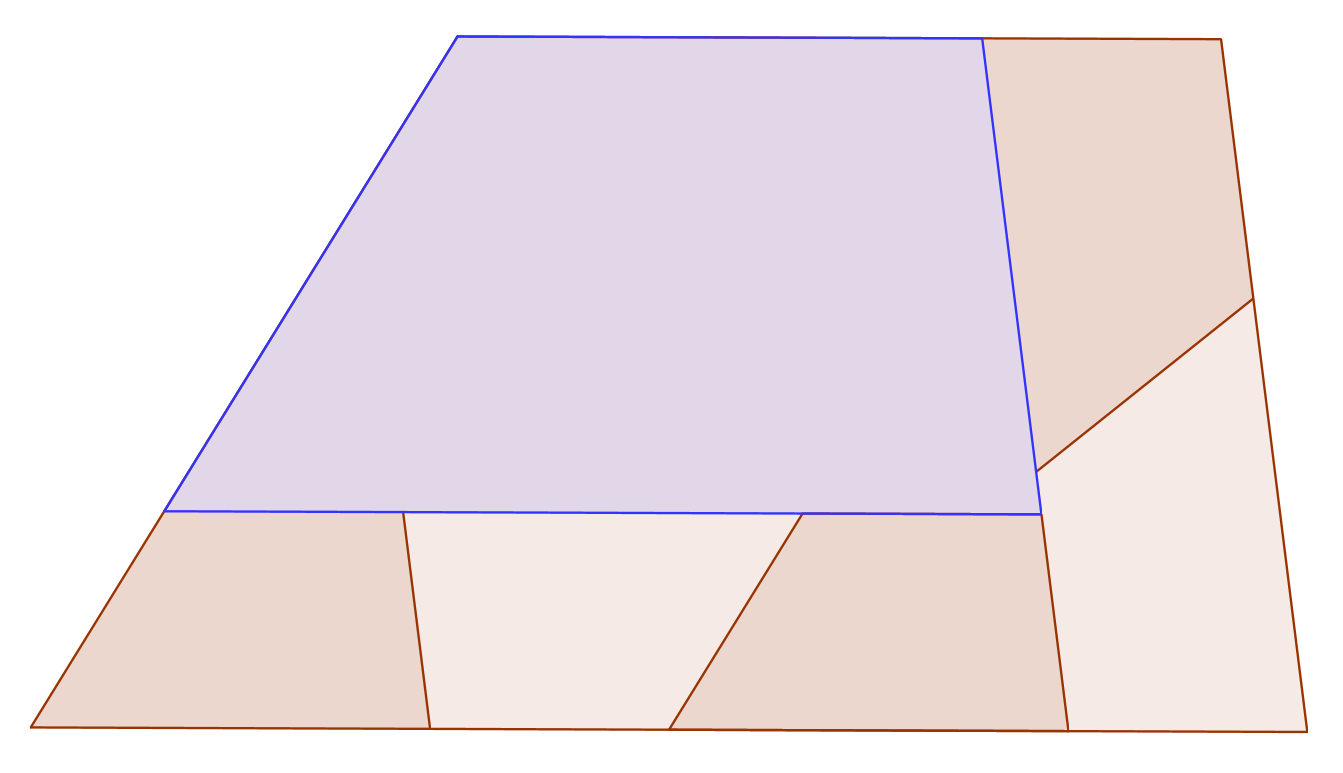
\includegraphics[height=1.6in]{images/T23} \hfill\par\vfill
    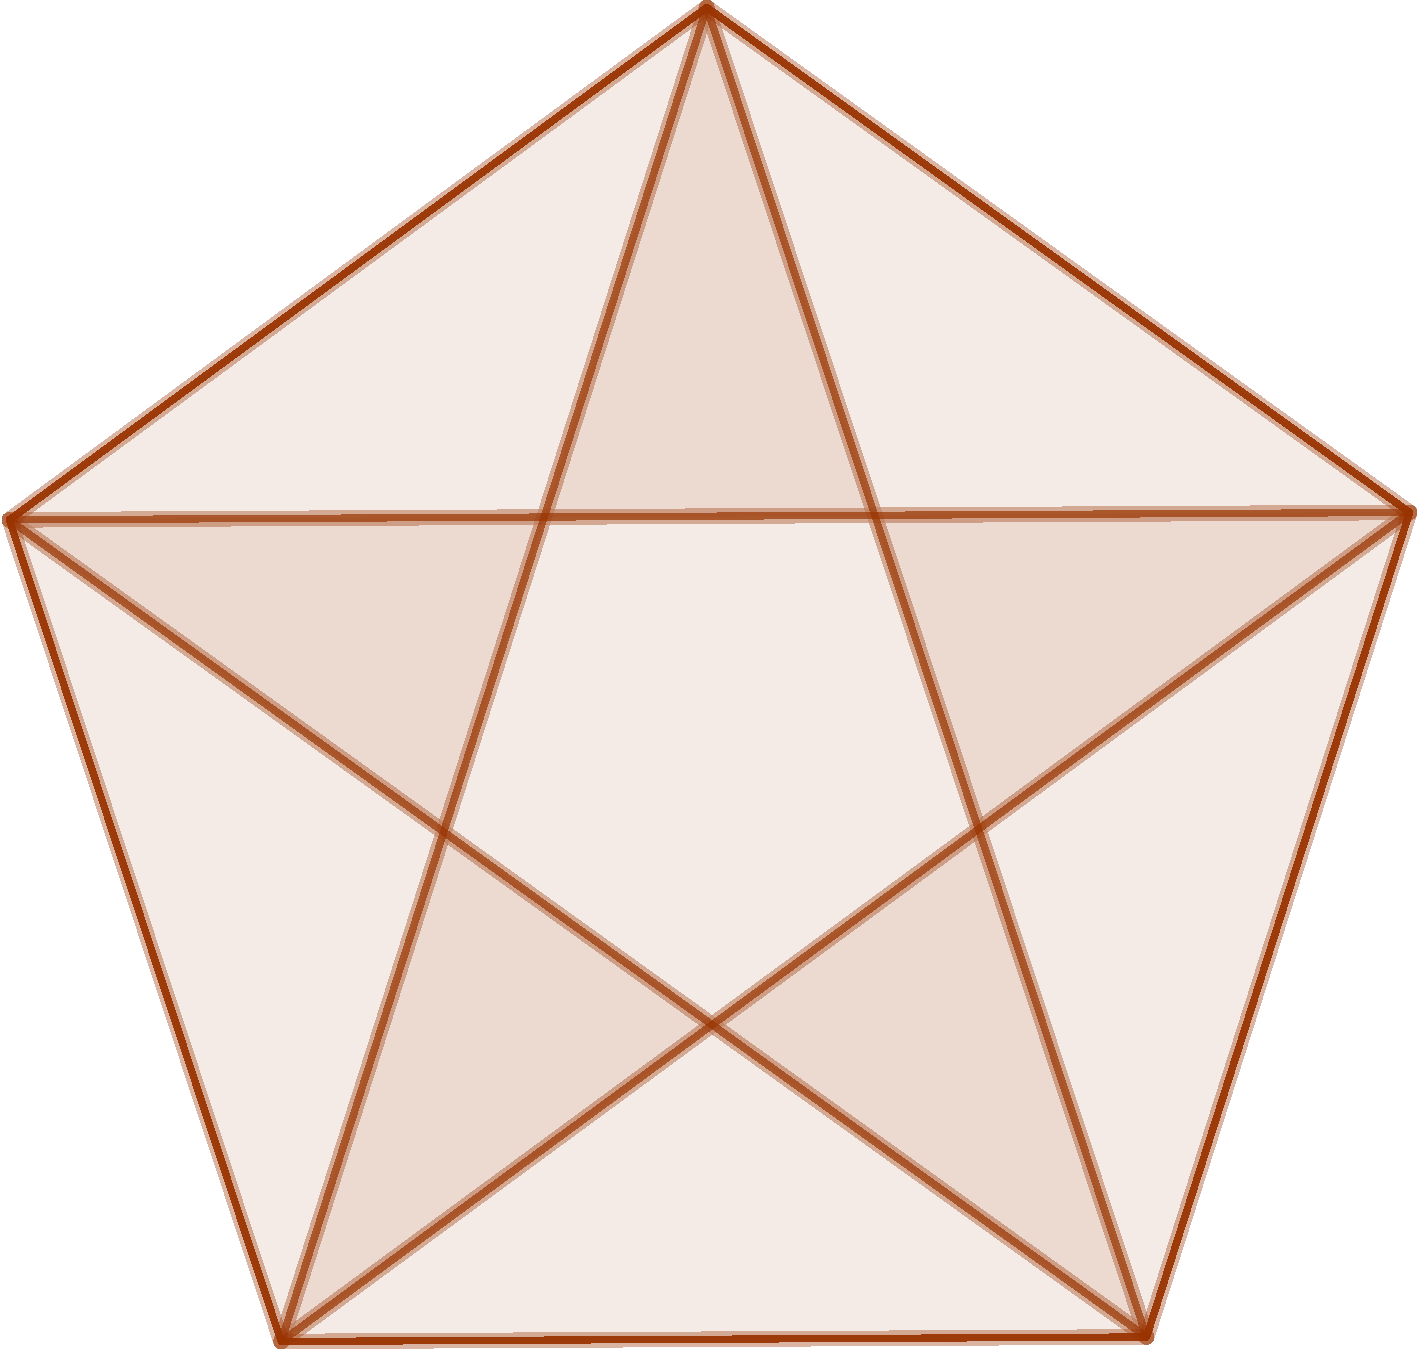
\includegraphics[height=1.6in]{images/pentagon} \hfill\par\vfill
    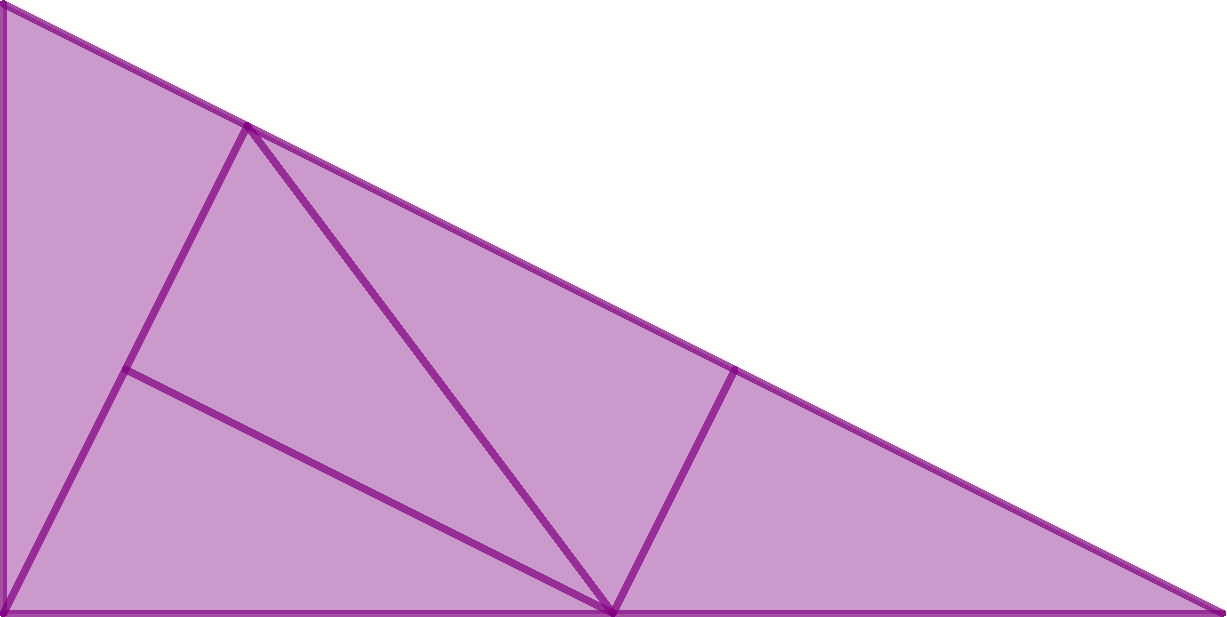
\includegraphics[height=1.6in]{images/rep-tile-74} 
    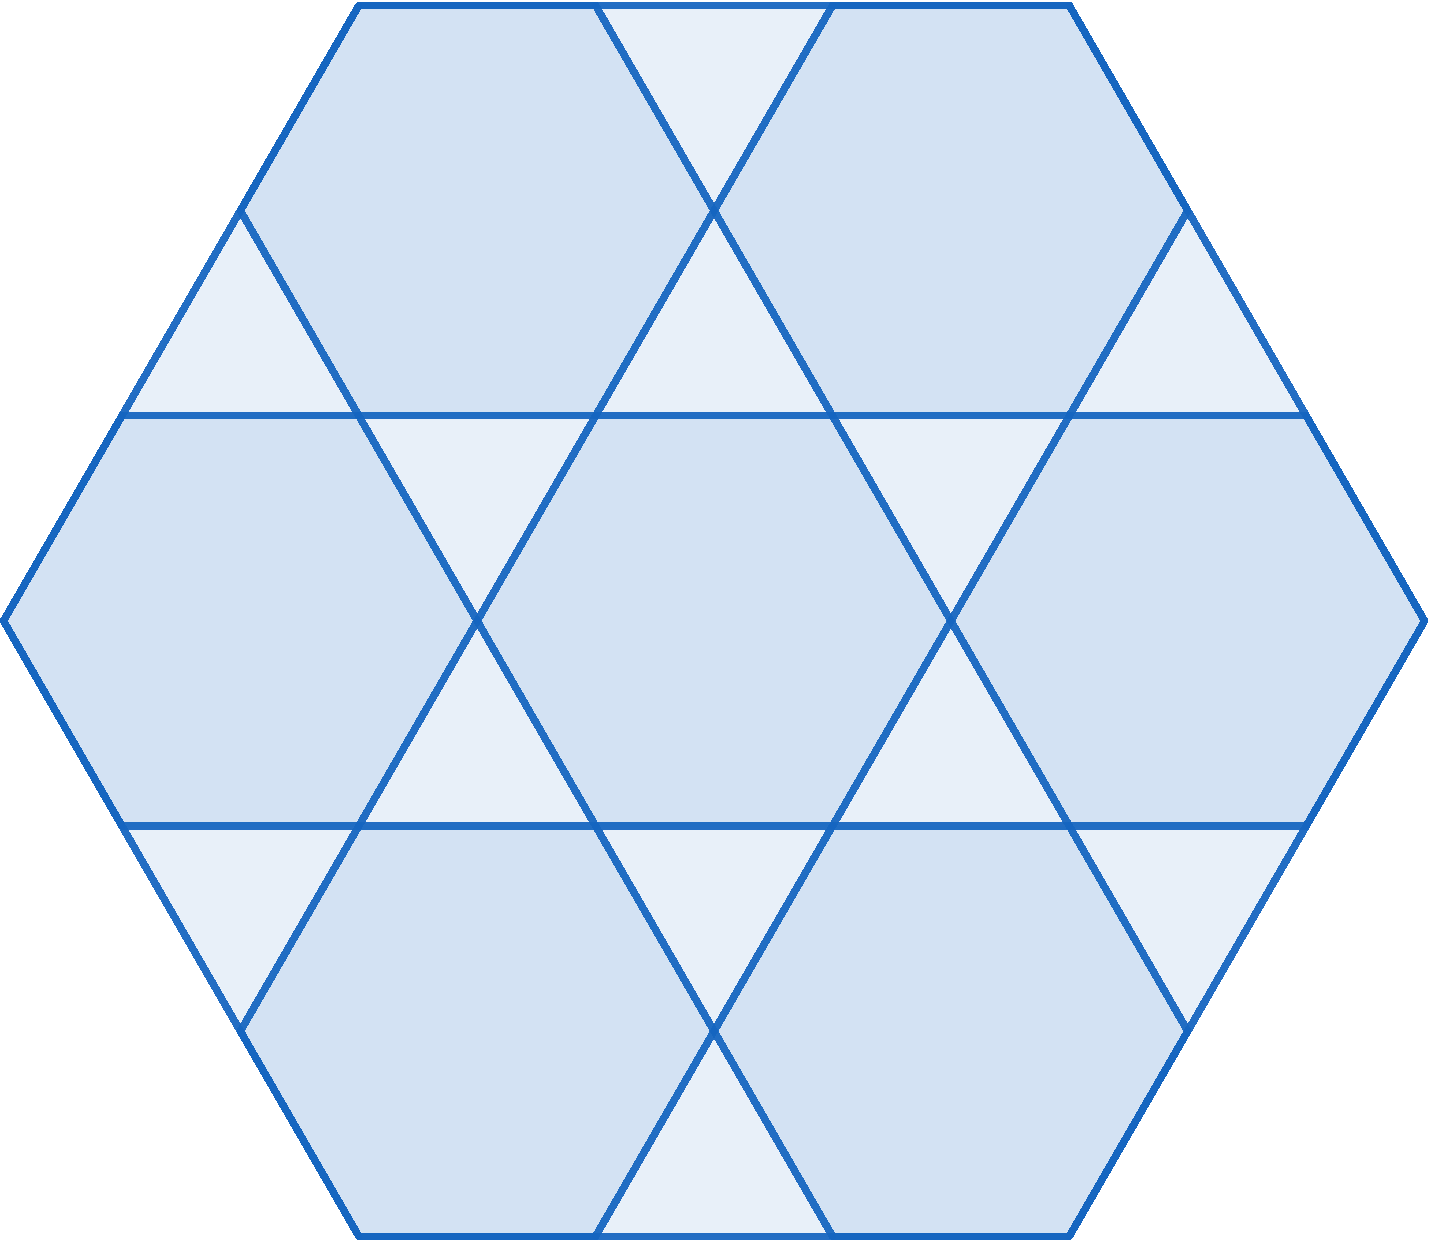
\includegraphics[height=1.6in]{images/hexagon-crop} \hfill
\end{center}
\Instr{  The pentagon and hexagon are NOT rep-tiles. Each one is built up from shapes that are not similar to the whole. In the pentagon, there is a pentagon, but there are also triangles, and triangles are not similar to a regular pentagon. In the hexagon, there are 7 hexagons, but there are also triangles, and triangles are not similar to a regular hexagon. Even though it may not be obvious from a cursory glance, the trapezoid is built from dilated copies of itself so it is a rep-tile. The fact that the pieces used to build the whole are not congruent does not matter.}
\item Pieces to assemble four different rep-tiles appear below. Cut out the pieces and see how many of the four rep-tiles you can fit together.
\begin{center}
    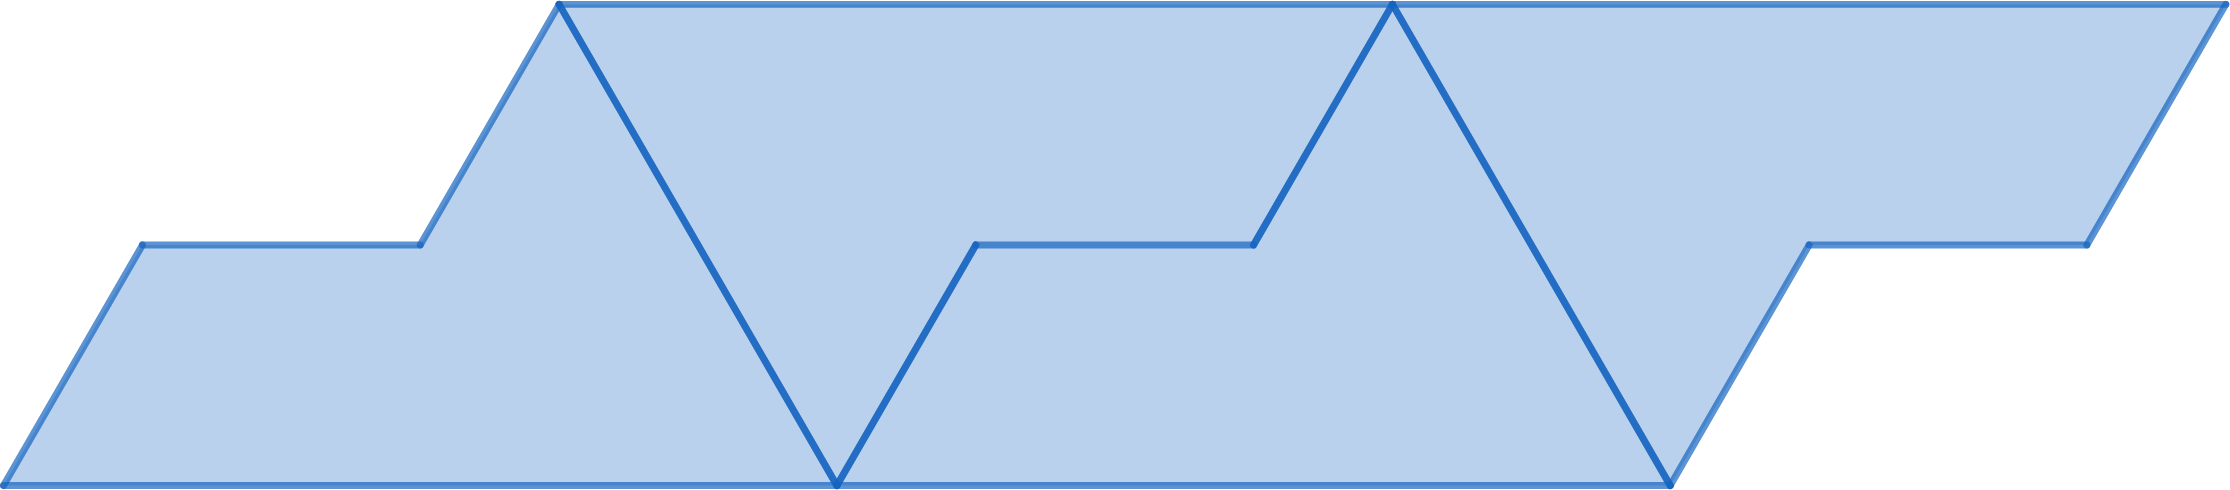
\includegraphics[width=5.5in]{images/rep-tile-02} \vfill
    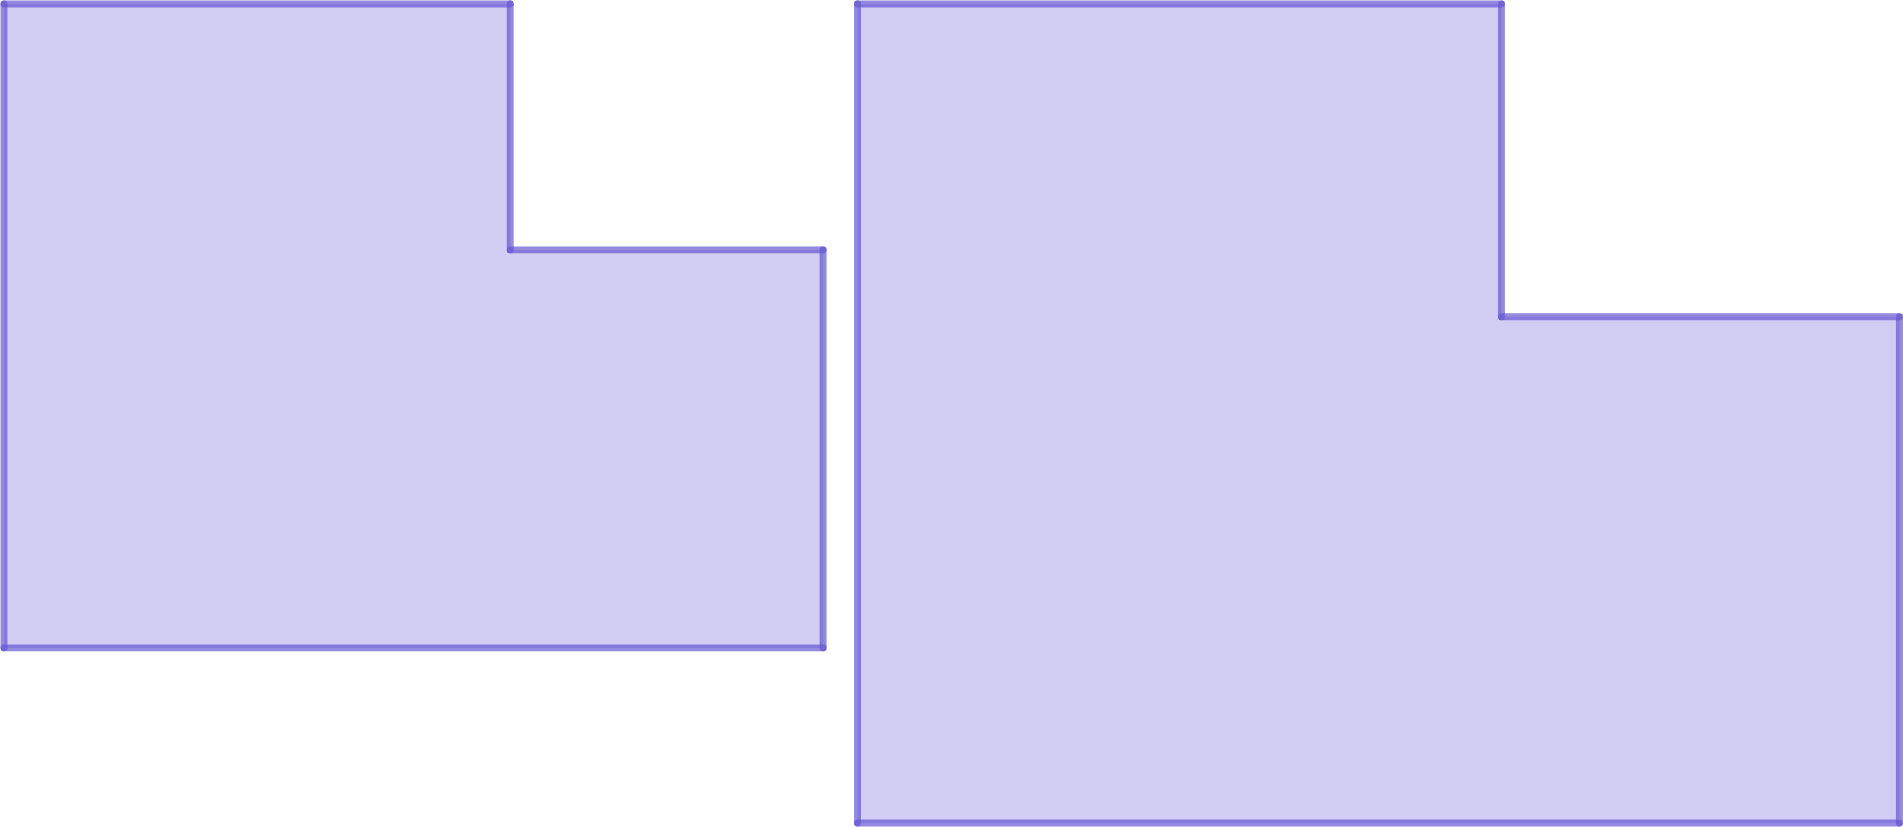
\includegraphics[width=4.5in]{images/rep-tile-10} \vfill
    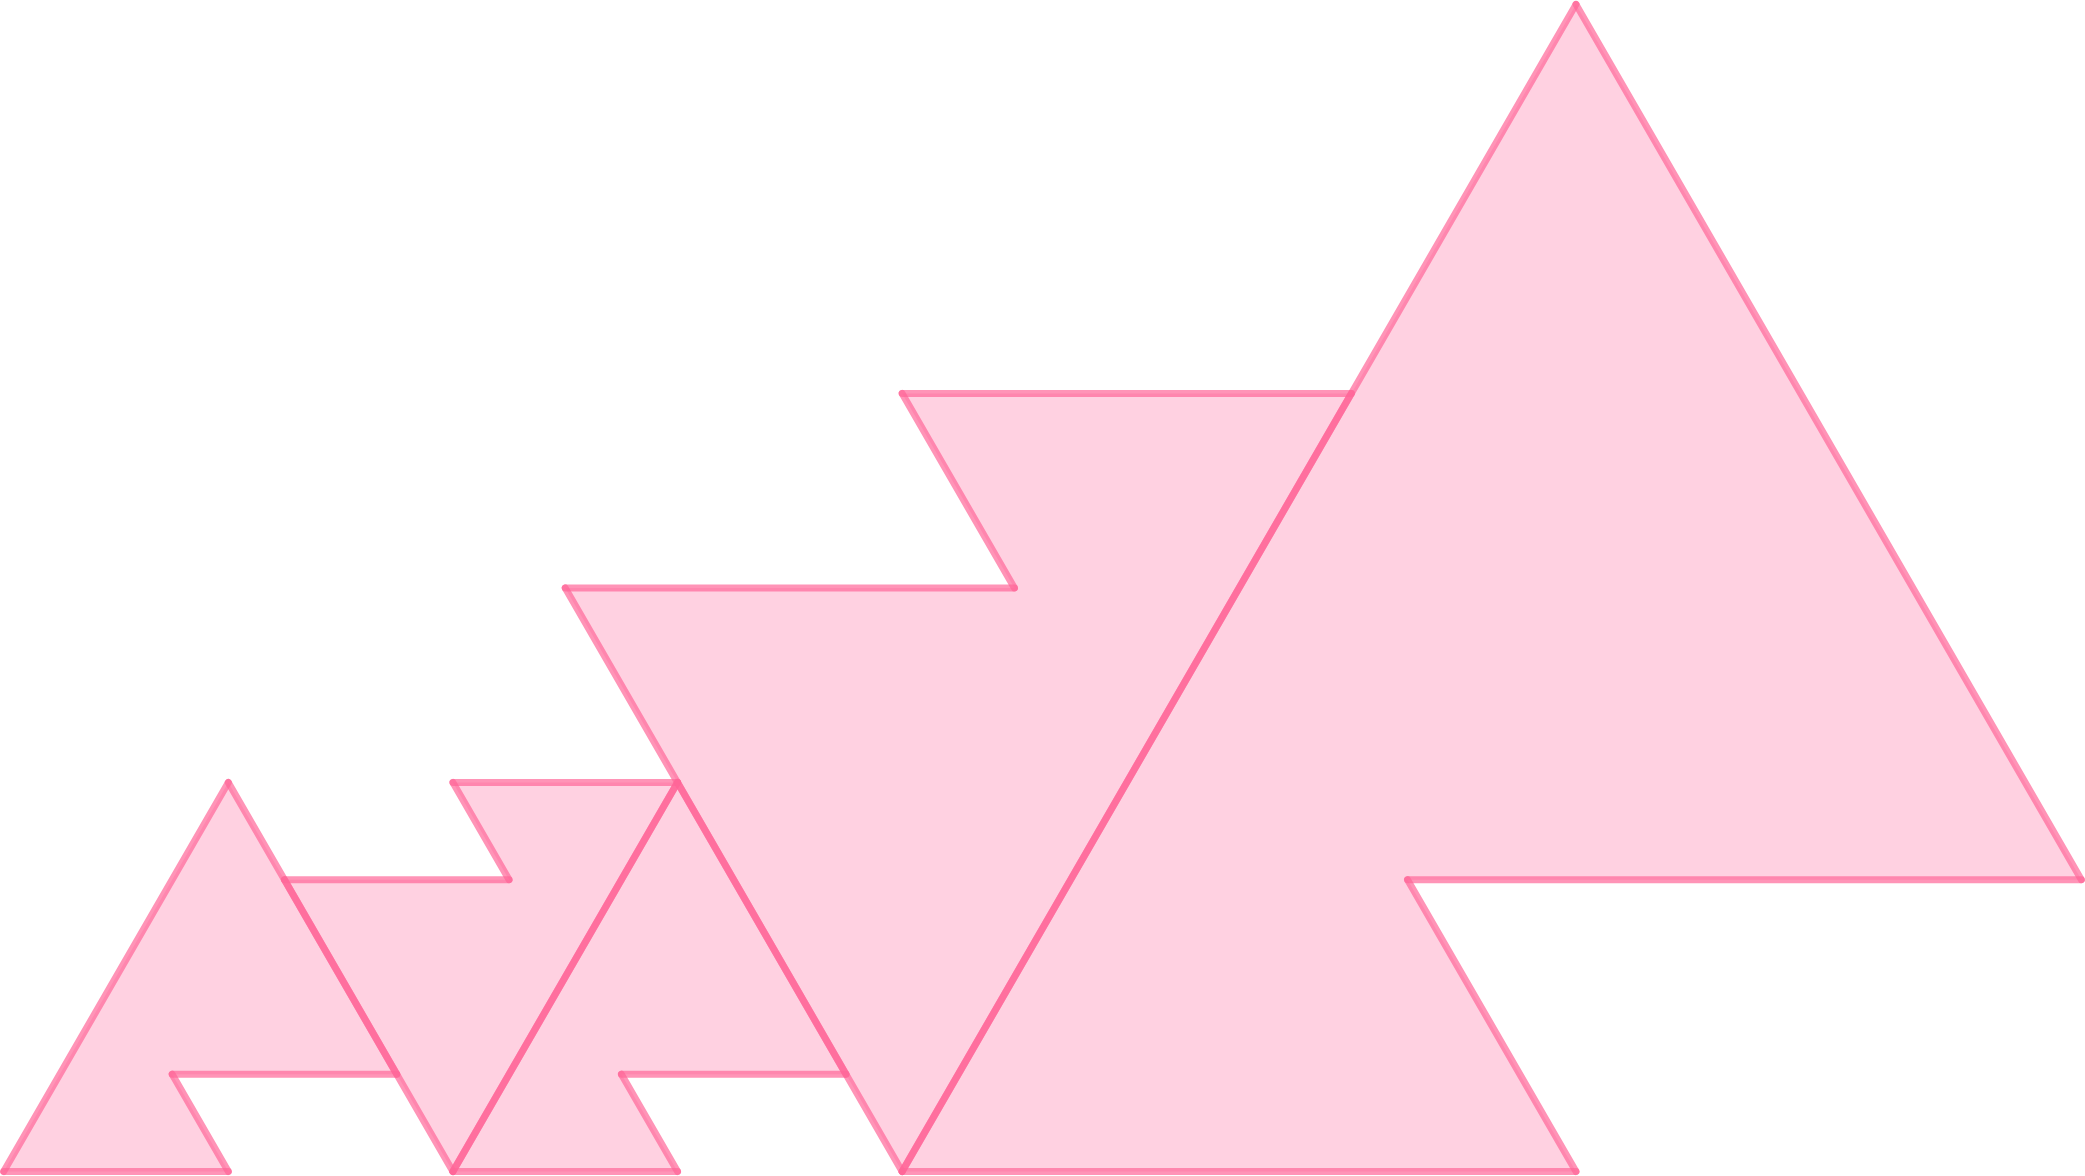
\includegraphics[width=4.5in]{images/rep-tile-12} \vfill
    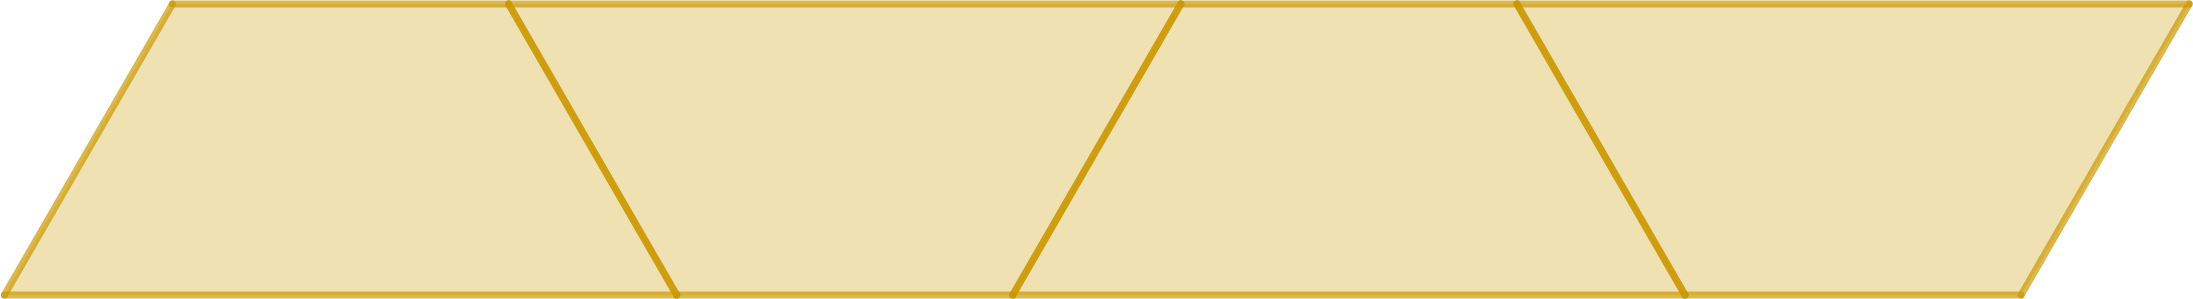
\includegraphics[width=5.5in]{images/rep-tile-18} \vfill
\end{center}
\Instr{  Here are their assemblies. In each case except the trapezoid, it is necessary to reflect at least one of the copies.
\begin{center}
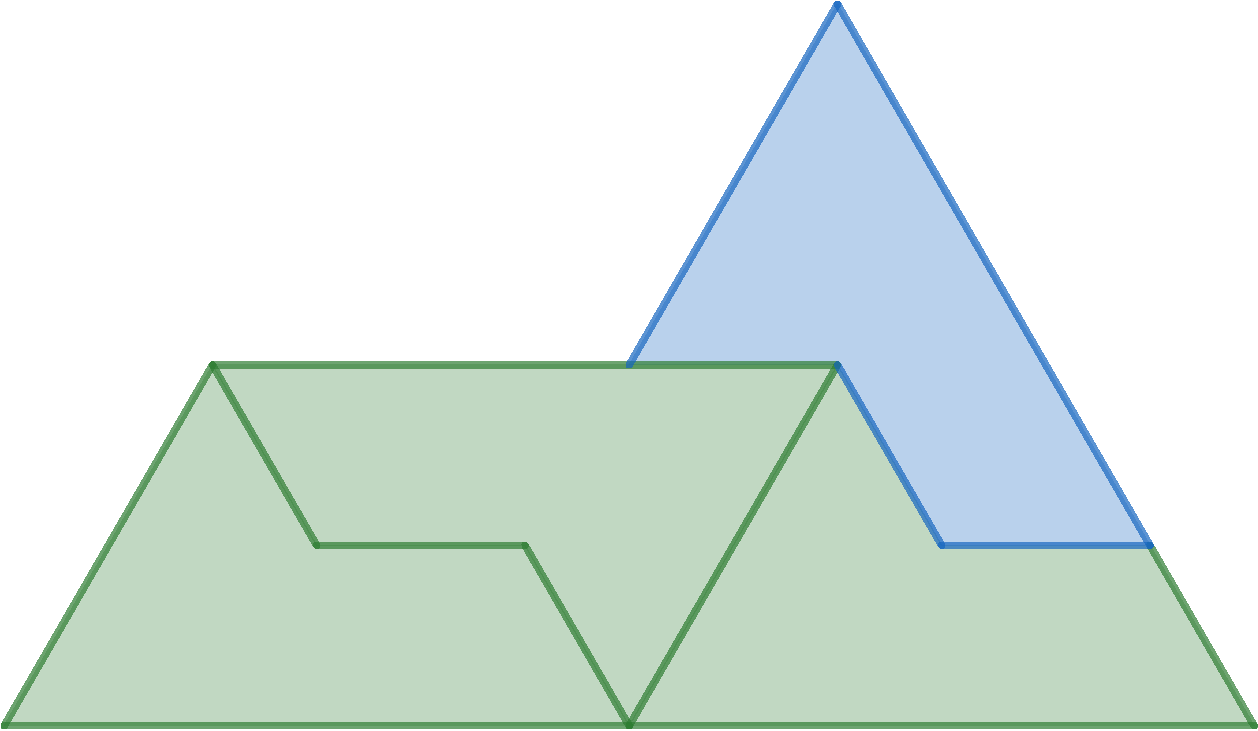
\includegraphics[height=1in]{images/sphynxAnswer}
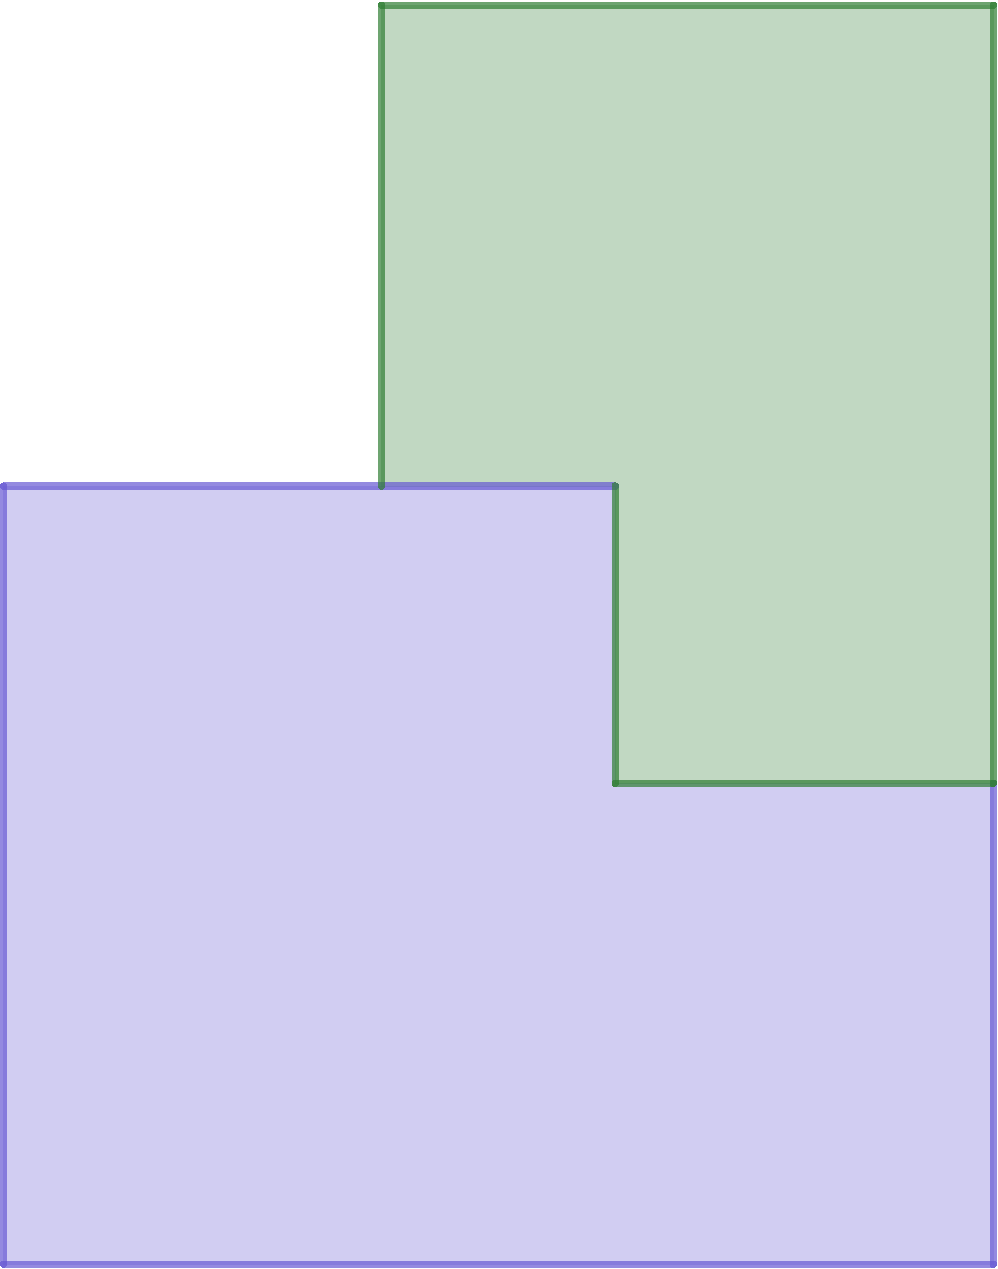
\includegraphics[height=1in]{images/chairAnswer}
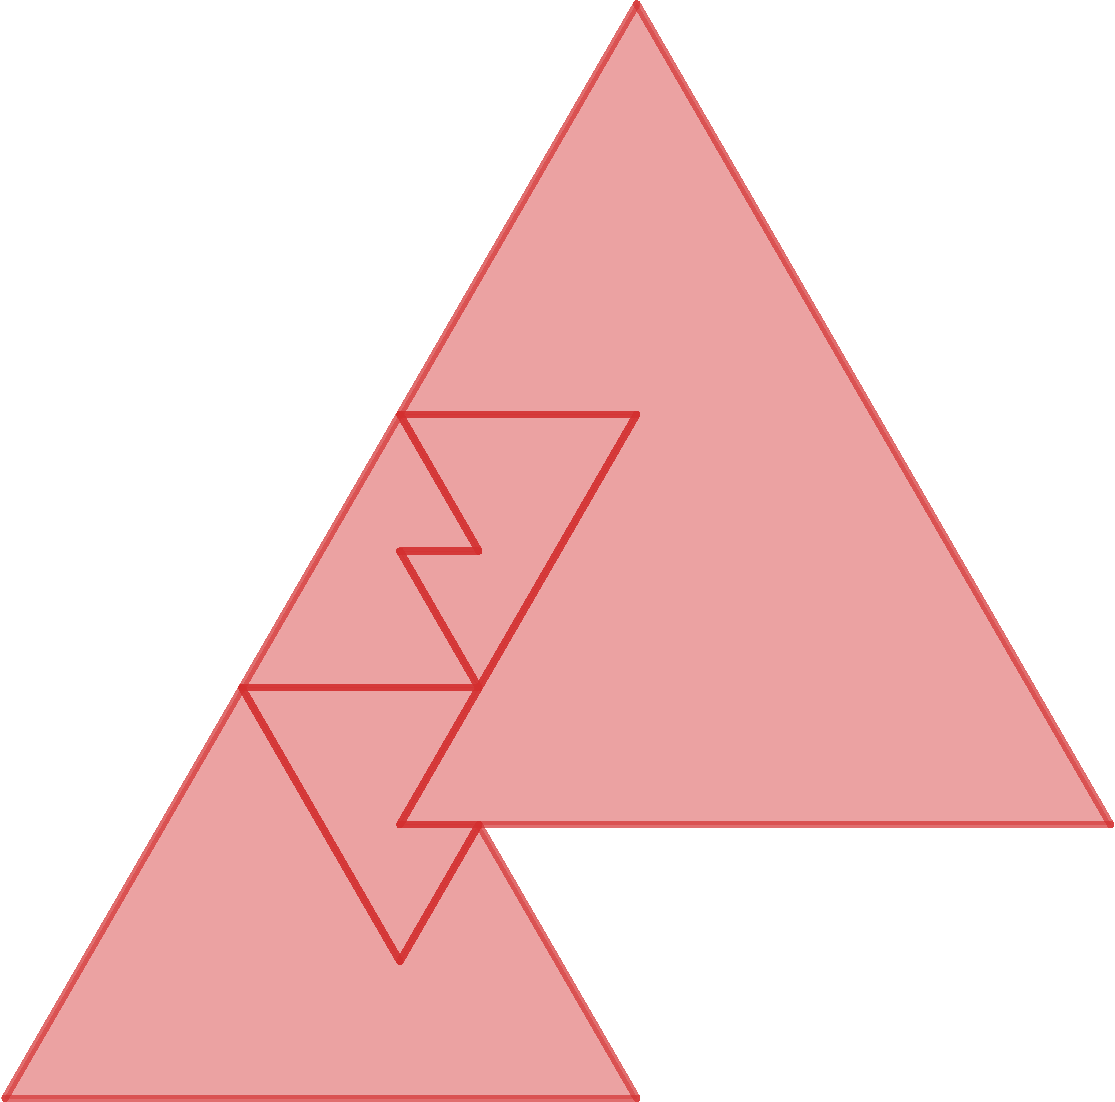
\includegraphics[height=1in]{images/pentagonAnswer}
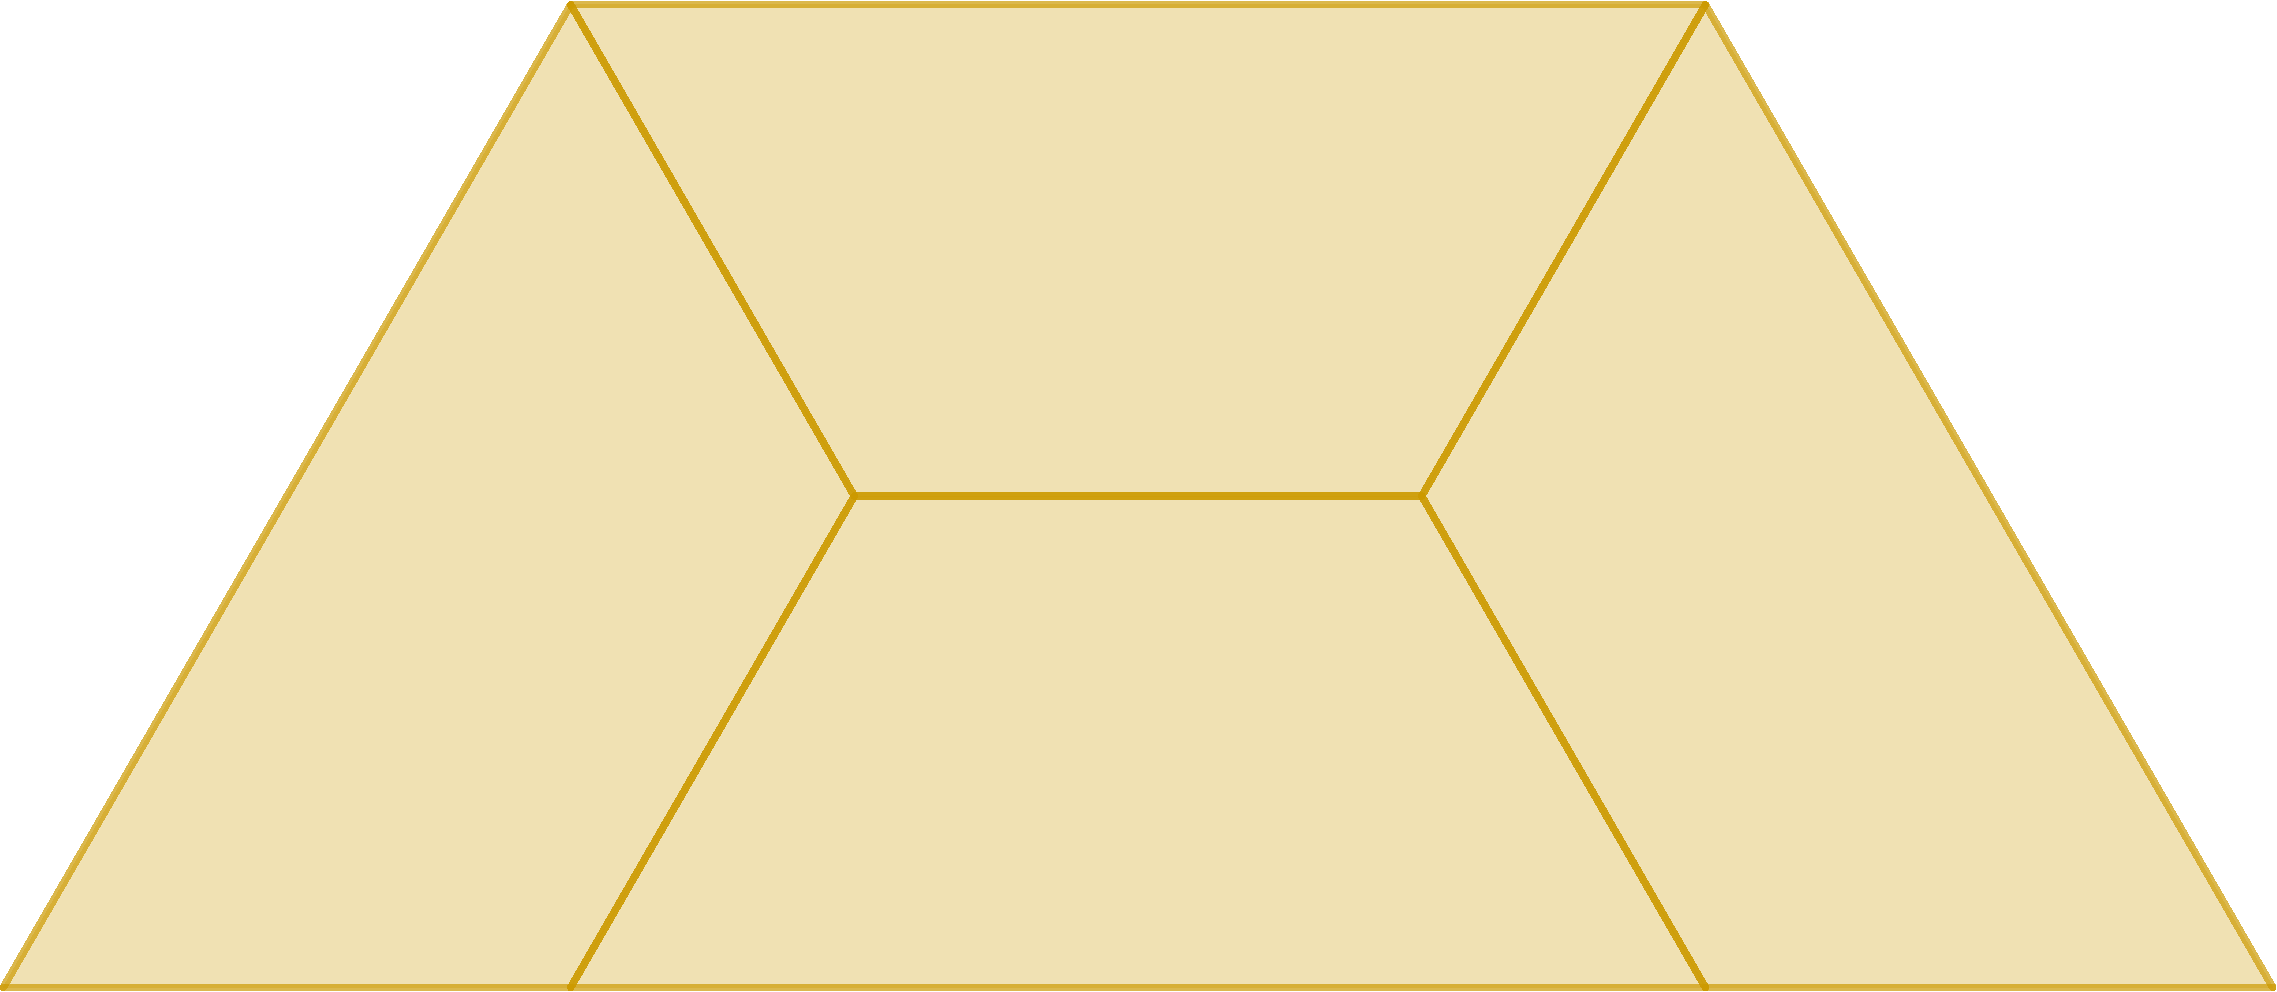
\includegraphics[height=.7in]{images/trapezoidAnswer}
\end{center}
}
\end{enumerate}
\wbnewpage

\subsection{Activity: Defining a rep-tile}
\Instr{ It would be a good idea to have students bring laptops to class for the last question of this activity.}

You've probably heard the phrases "two points define a line" or "a circle is defined by its center and radius". One way to understand what we mean by "define" in these two phrases is that the information describes exactly one line or one circle. For any two points, there is exactly one line that passes through both. For every center-radius pair there is exactly one circle with that center and radius. In the same way, a rep-tile is defined by the relationships between its parts and the whole. If we can precisely describe these relationships, there will be exactly one rep-tile with that description. Take the rep-tile below.
\begin{center}
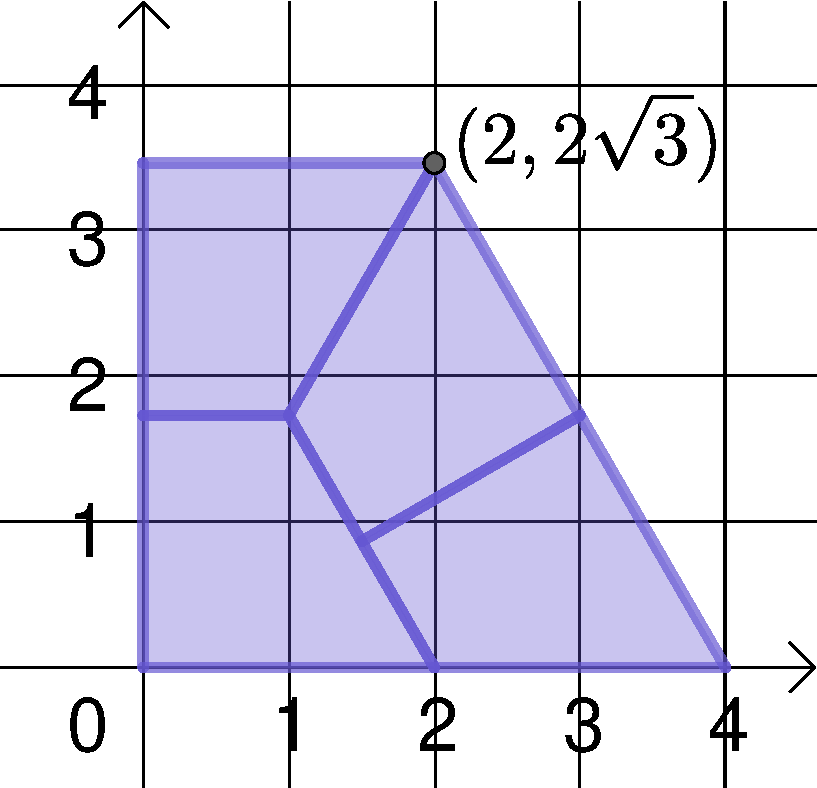
\includegraphics[height=2in]{images/rt-trap}
\end{center}
It is a trapezoid formed by fitting together four similar trapezoids. With the axes superimposed on the rep-tile, we can mathematically describe the relationships between the parts and the whole in terms of dilations, rotations, reflections, and translations. For example, if we take the whole trapezoid and follow the steps below, it turns into one of the parts of the assembly.
\begin{center}
$\begin{array}{c} \text{start with}\\ \text{the whole} \end{array}$ \raisebox{-.75in}{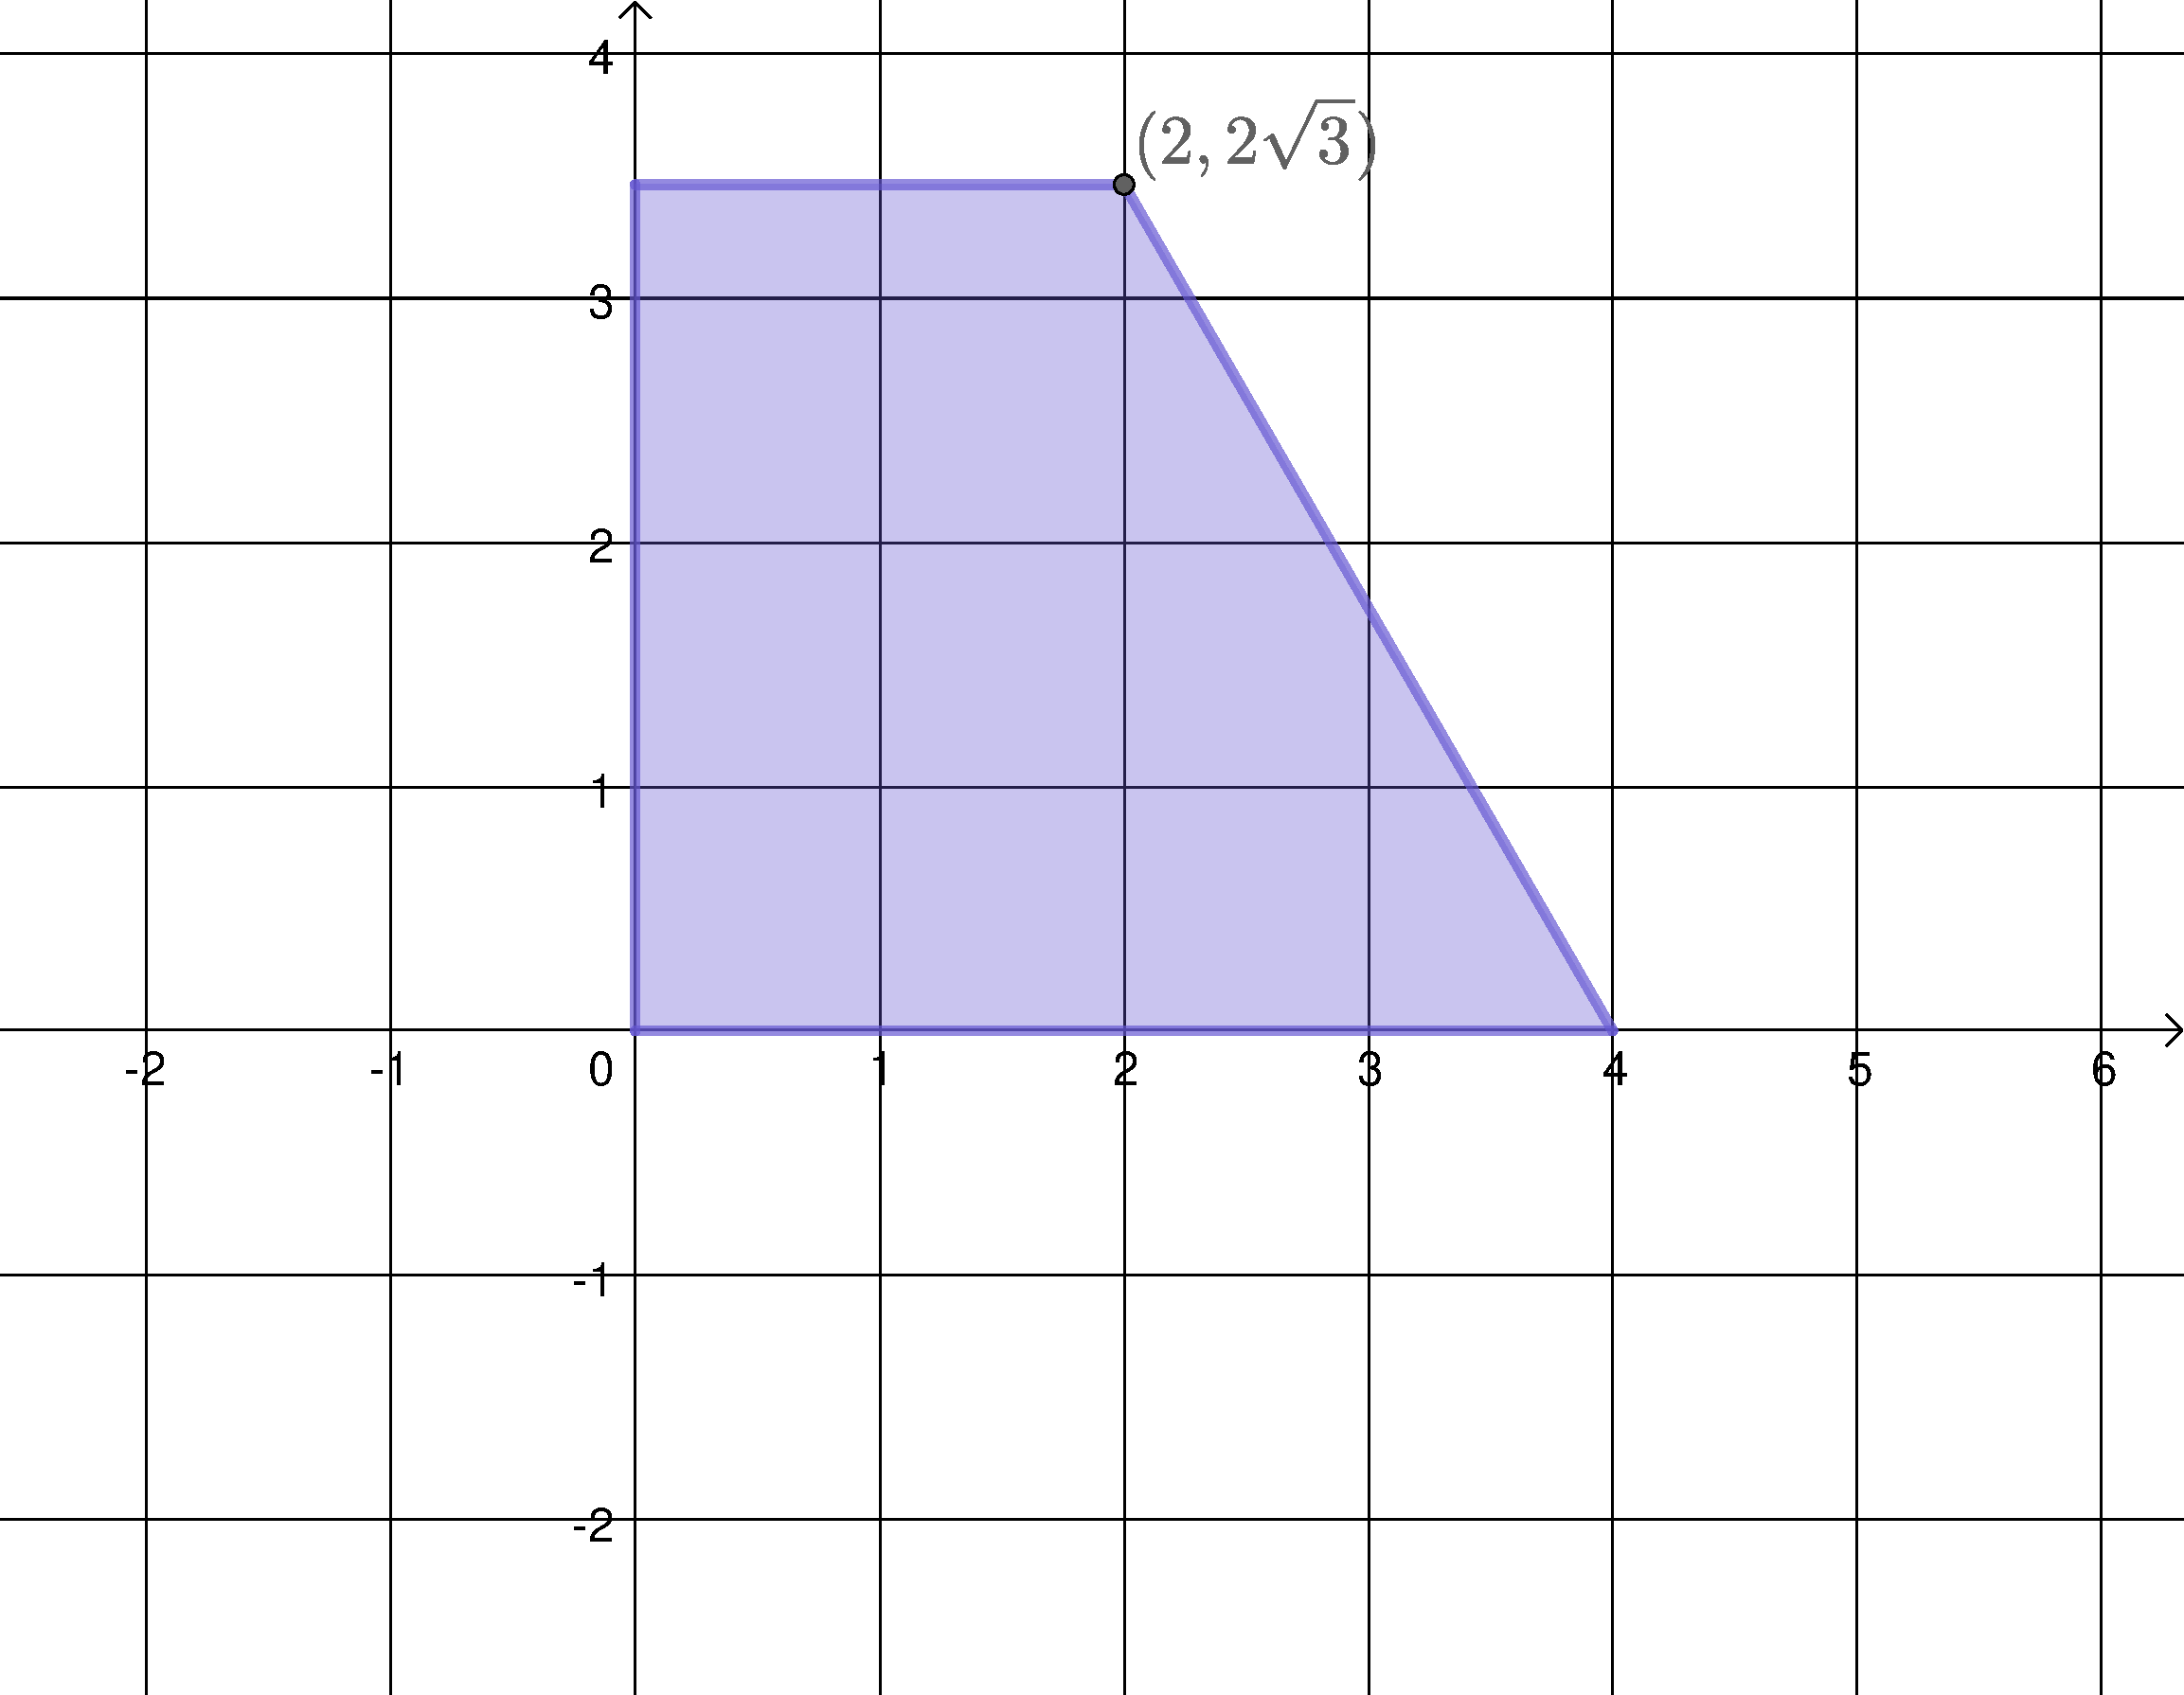
\includegraphics[width=1.75in]{images/rt-trap-start}}
$\begin{array}{c} \text{dilate }\\ \longrightarrow\\ \text{by }\frac12 \end{array}$ \raisebox{-.75in}{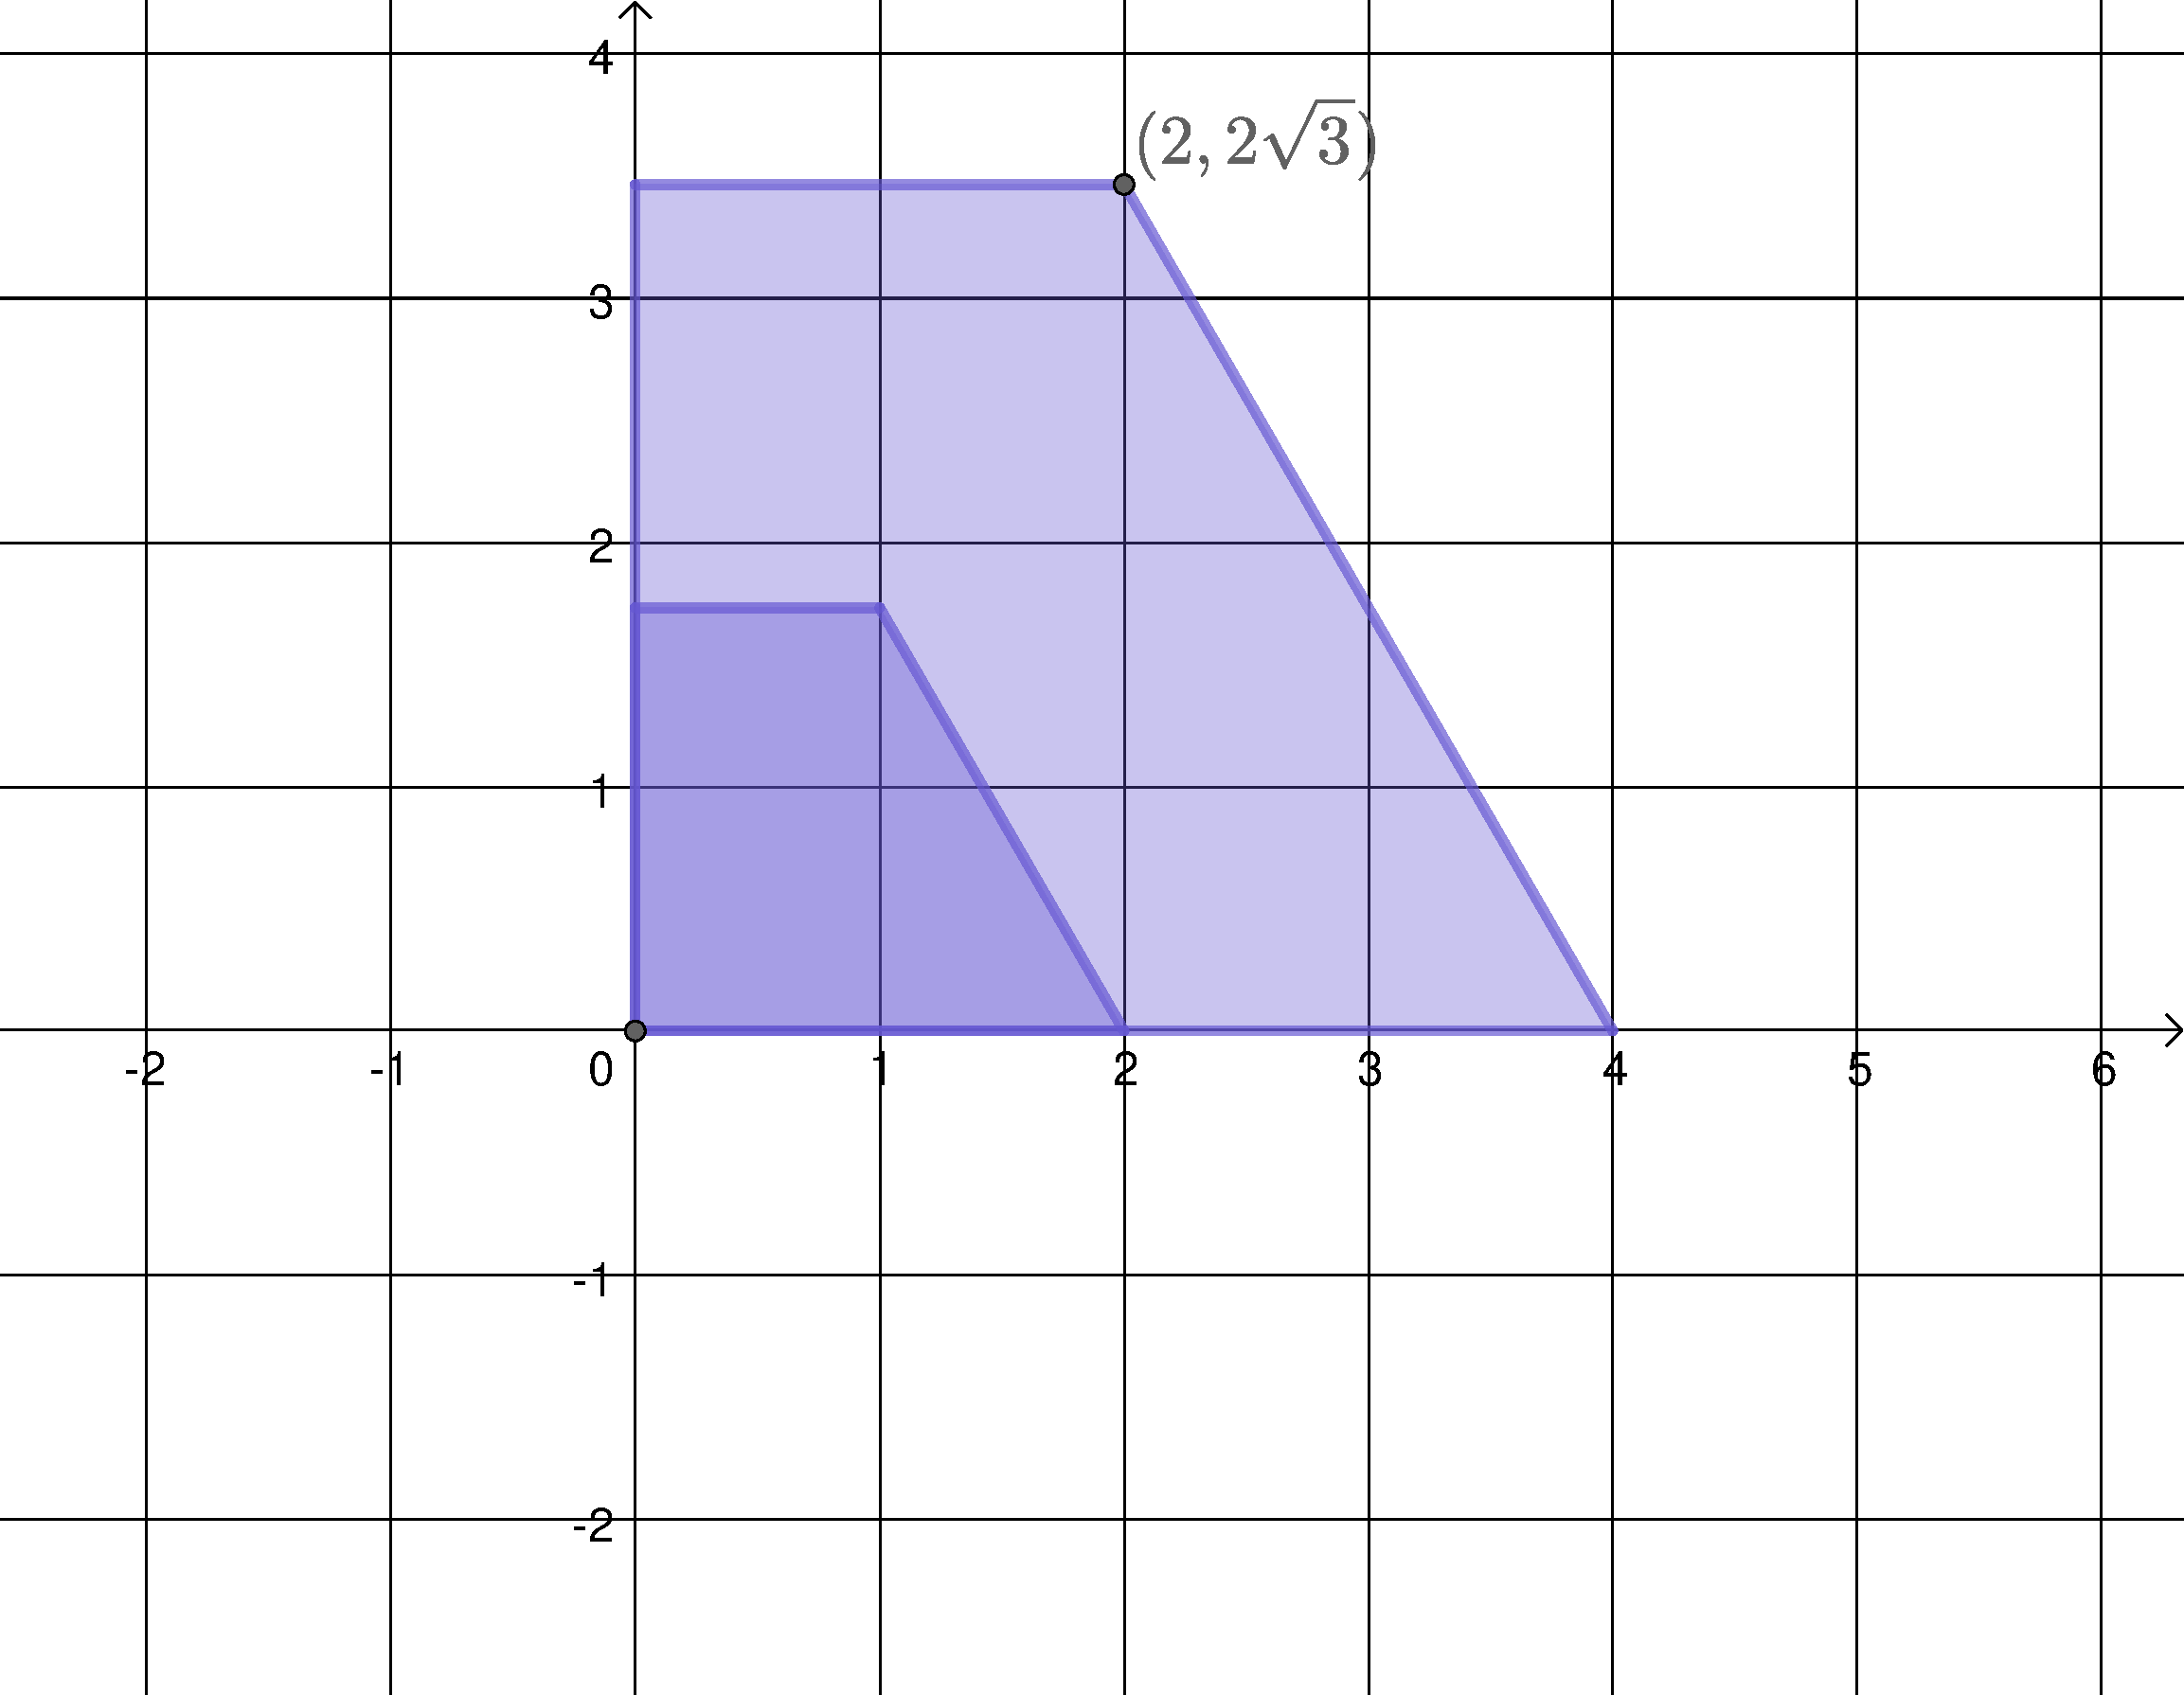
\includegraphics[width=1.75in]{images/rt-trap-scale}}\\
$\begin{array}{c} \text{rotate}\\ \longrightarrow\\ 120^\circ \end{array}$ \raisebox{-.75in}{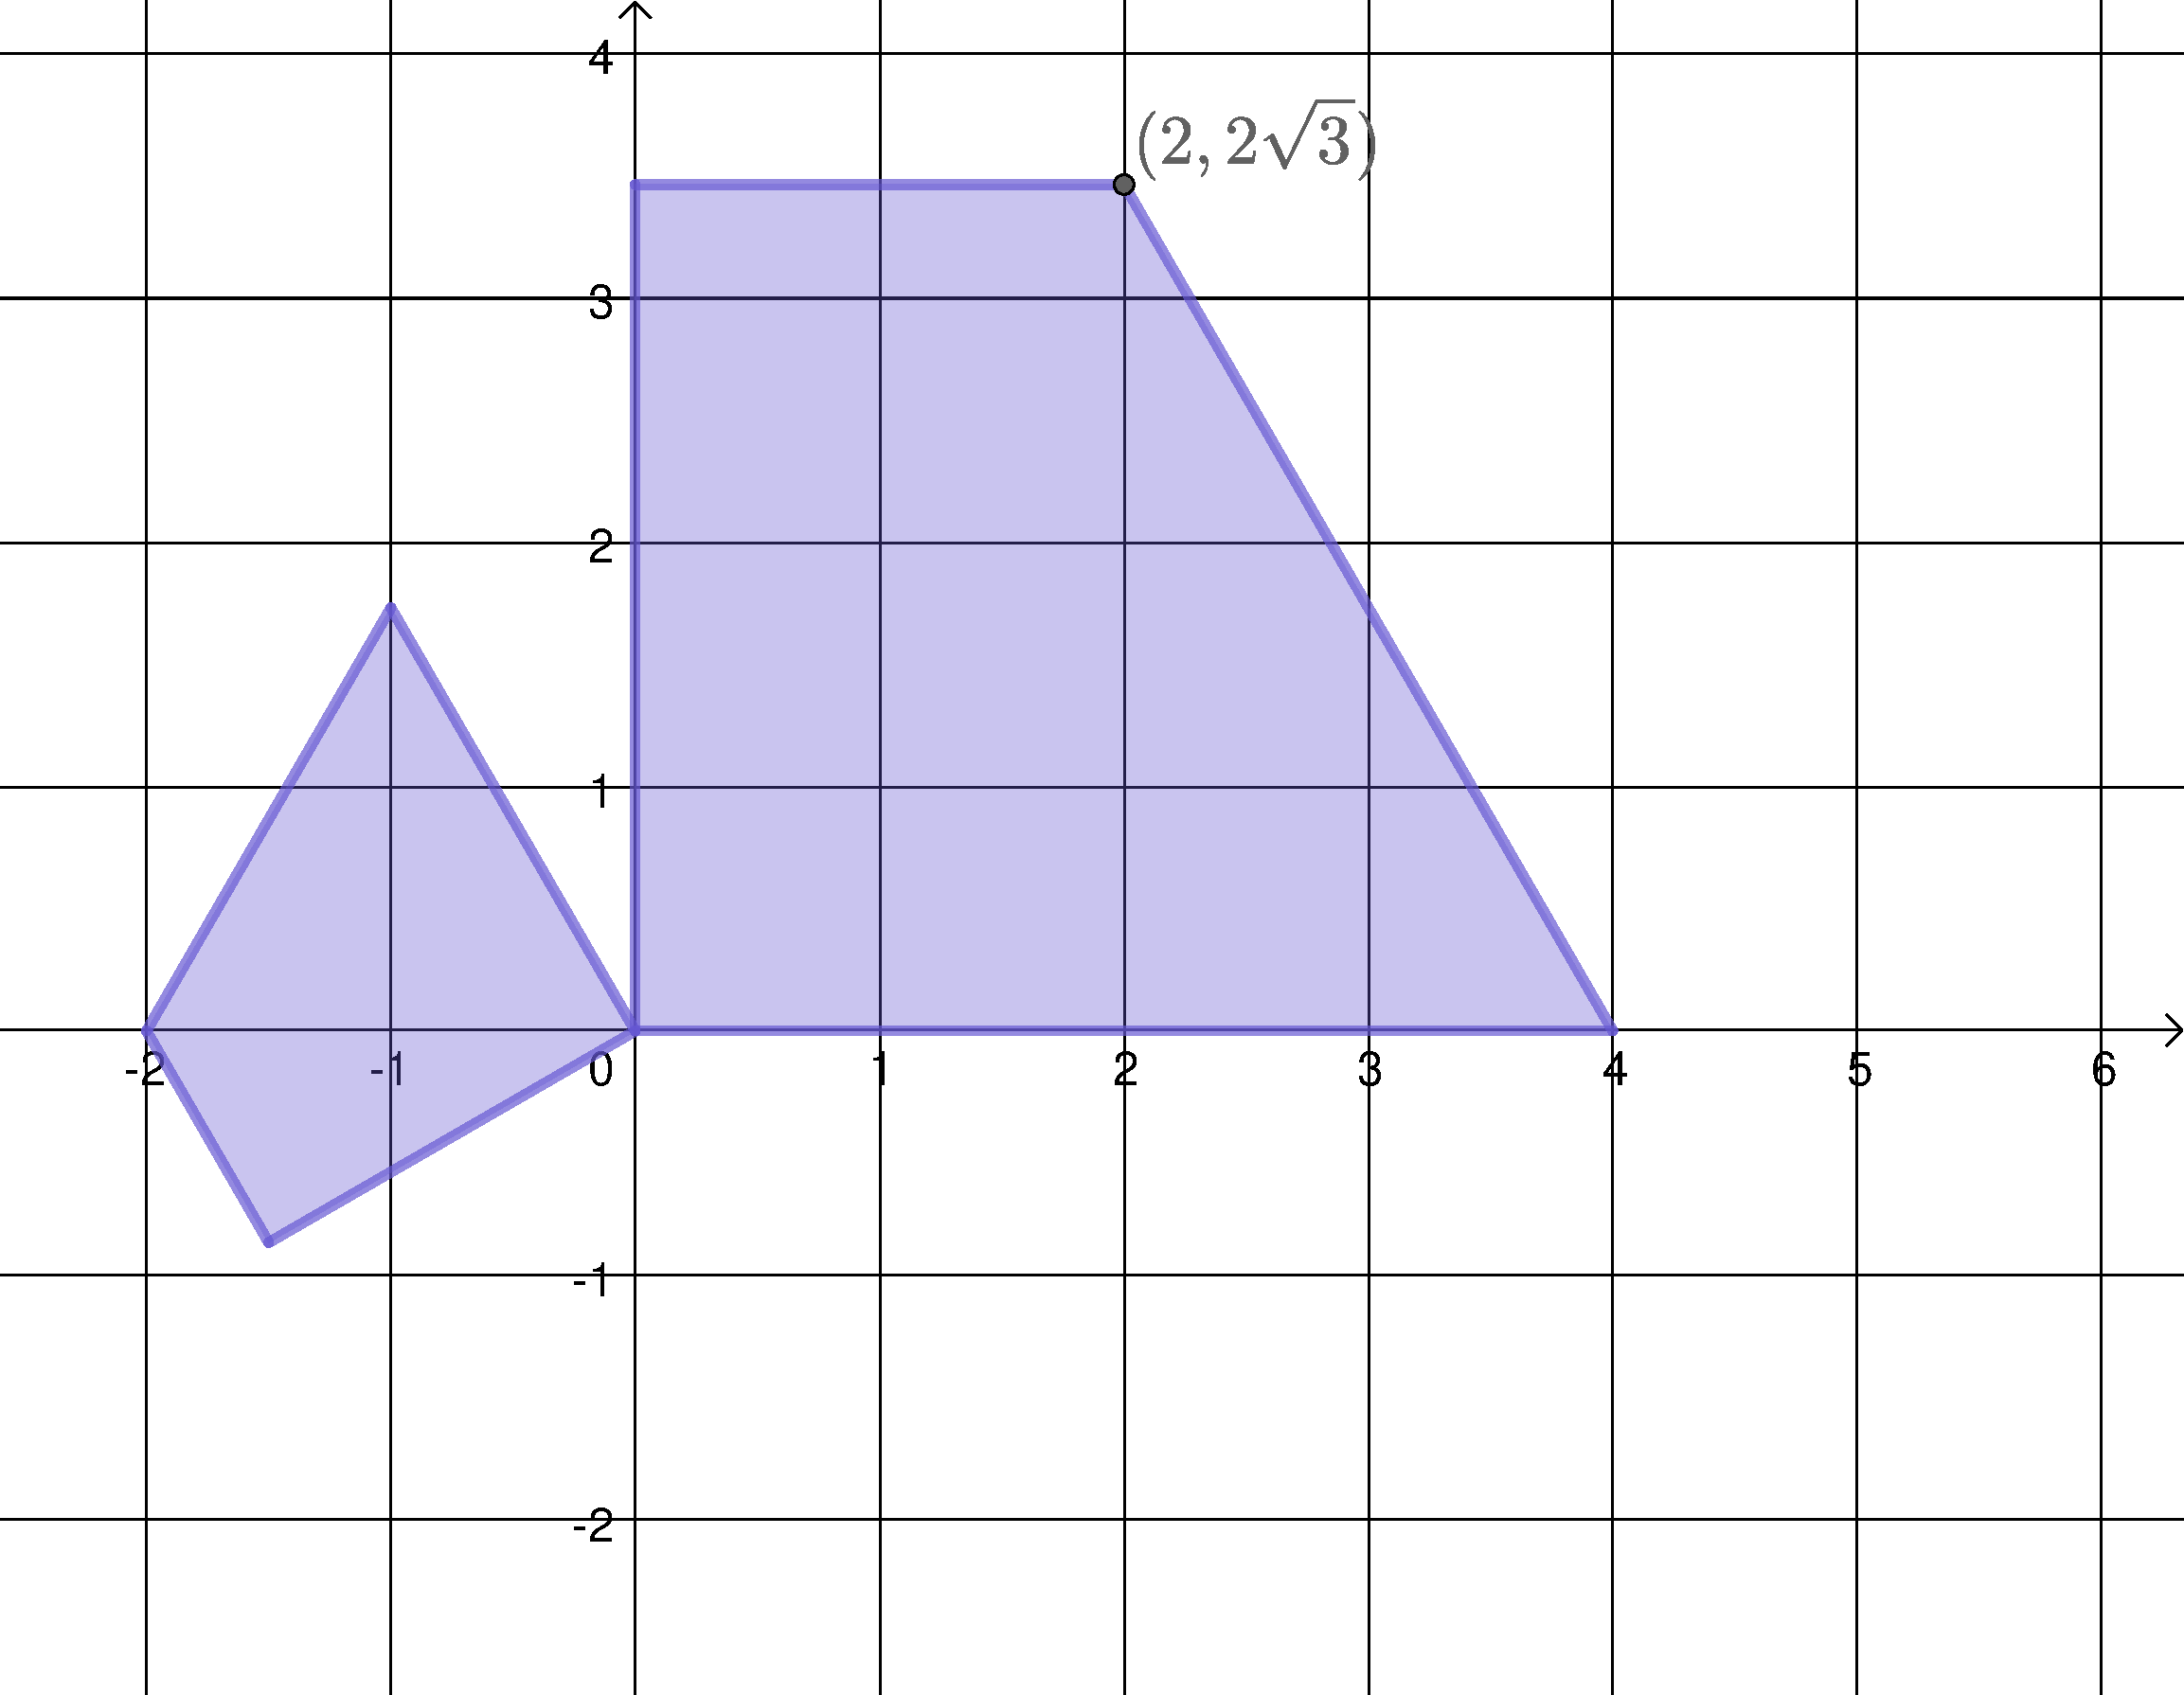
\includegraphics[width=1.75in]{images/rt-trap-scale-rotate}}
$\begin{array}{c} \text{translate}\\ \longrightarrow\\ (3,\sqrt{3}) \end{array}$ \raisebox{-.75in}{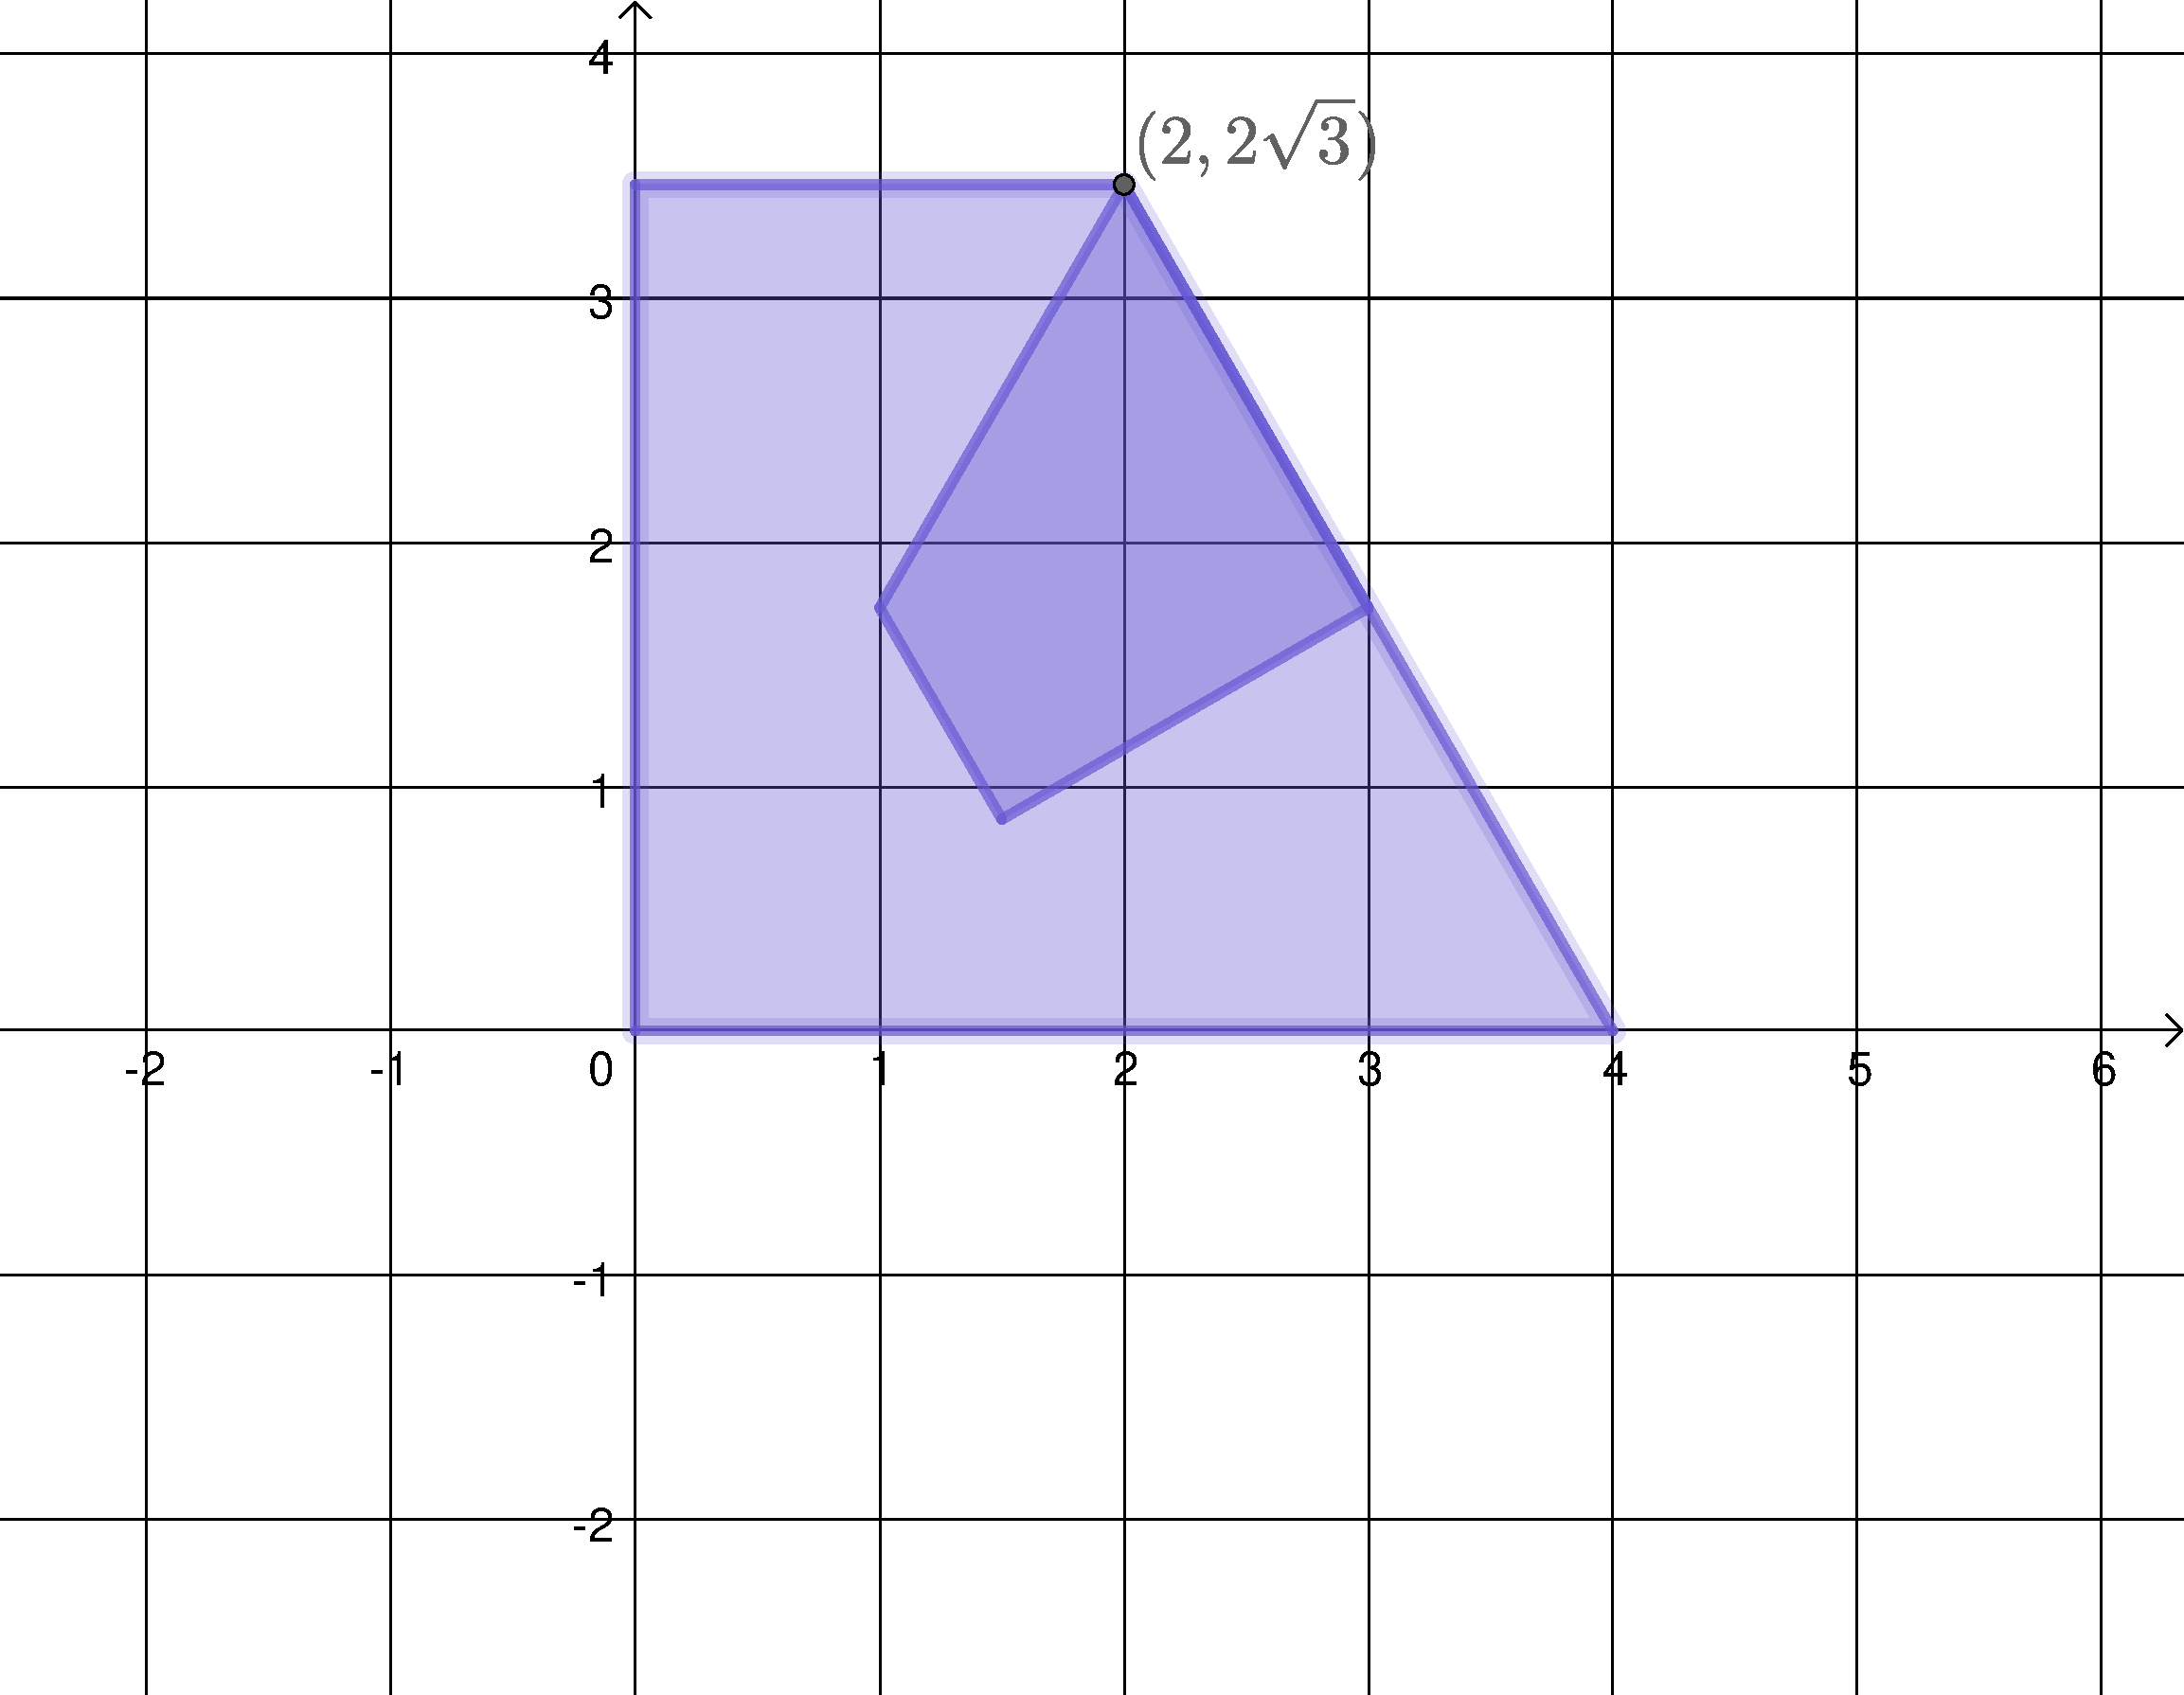
\includegraphics[width=1.75in]{images/rt-trap-part3}}
\par\end{center}
So ONE of the parts of the description that defines this rep-tile is
\textit{dilate by $\frac12$; rotate $120^\circ$; translate $(3,\sqrt3)$}. A second one is much simpler:
\begin{center}
$\begin{array}{c} \text{start with}\\ \text{the whole} \end{array}$ \raisebox{-.75in}{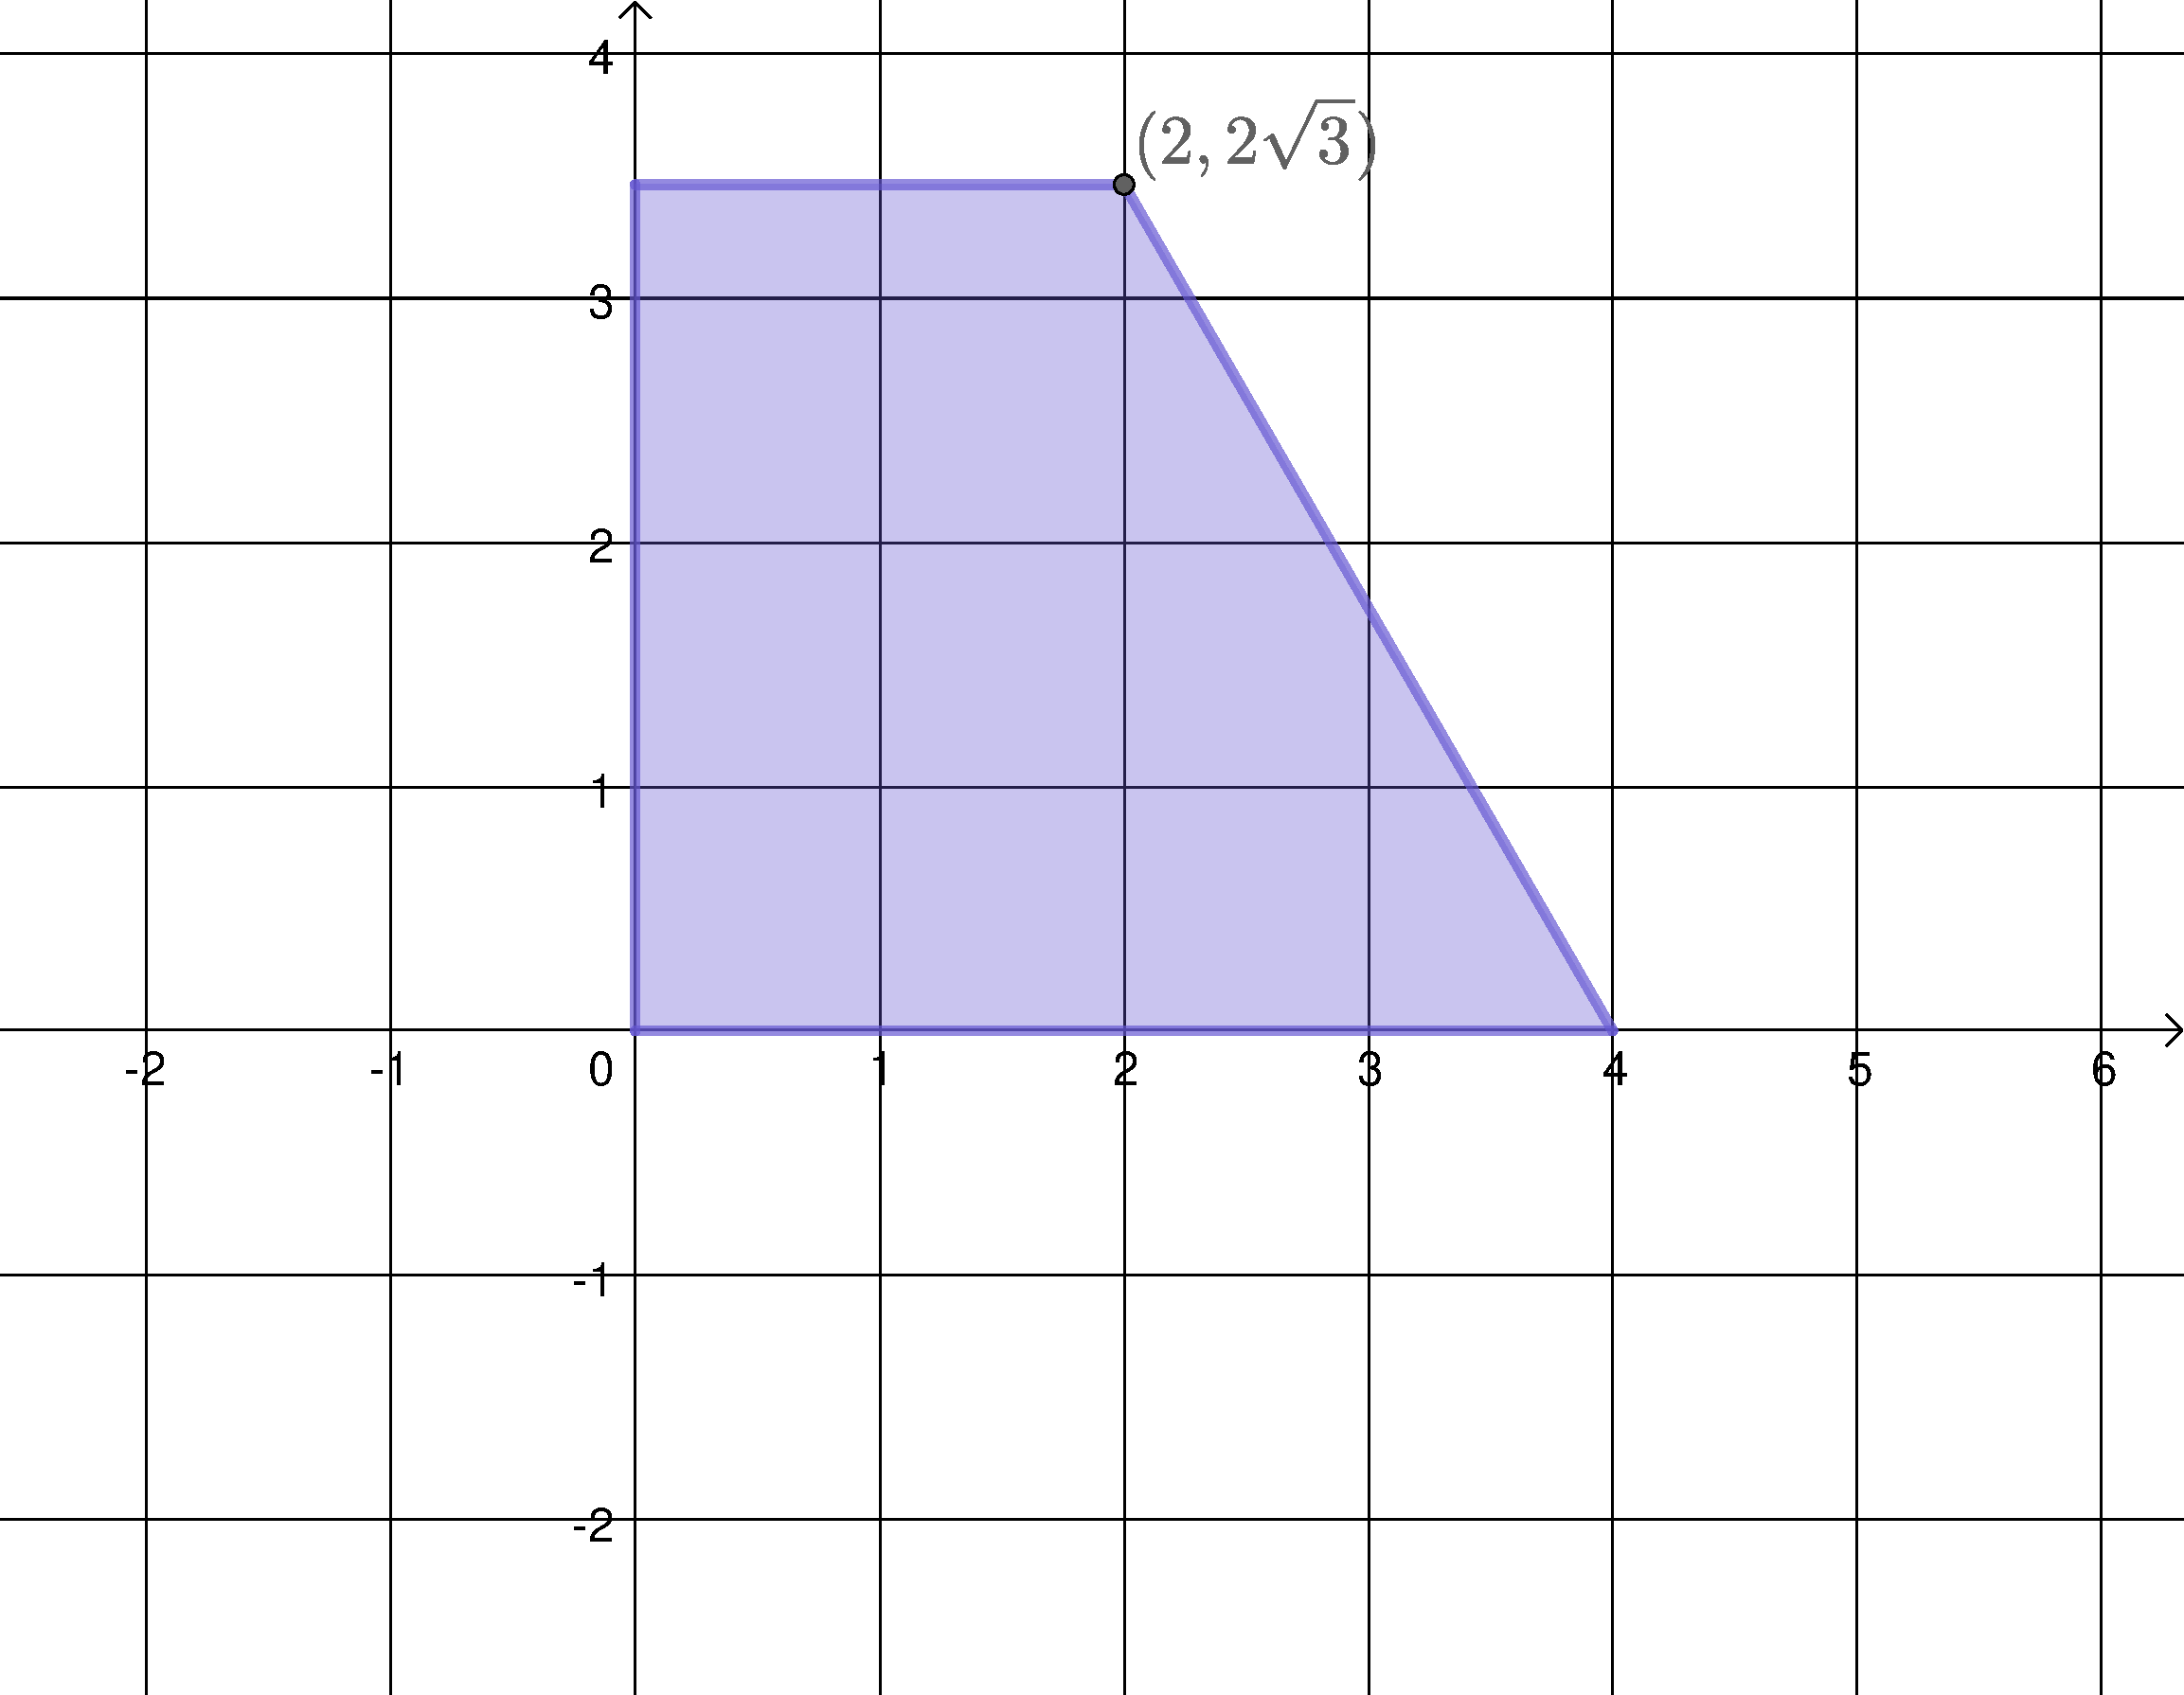
\includegraphics[width=1.75in]{images/rt-trap-start}}
$\begin{array}{c} \text{dilate }\\ \longrightarrow\\ \text{by }\frac12 \end{array}$ \raisebox{-.75in}{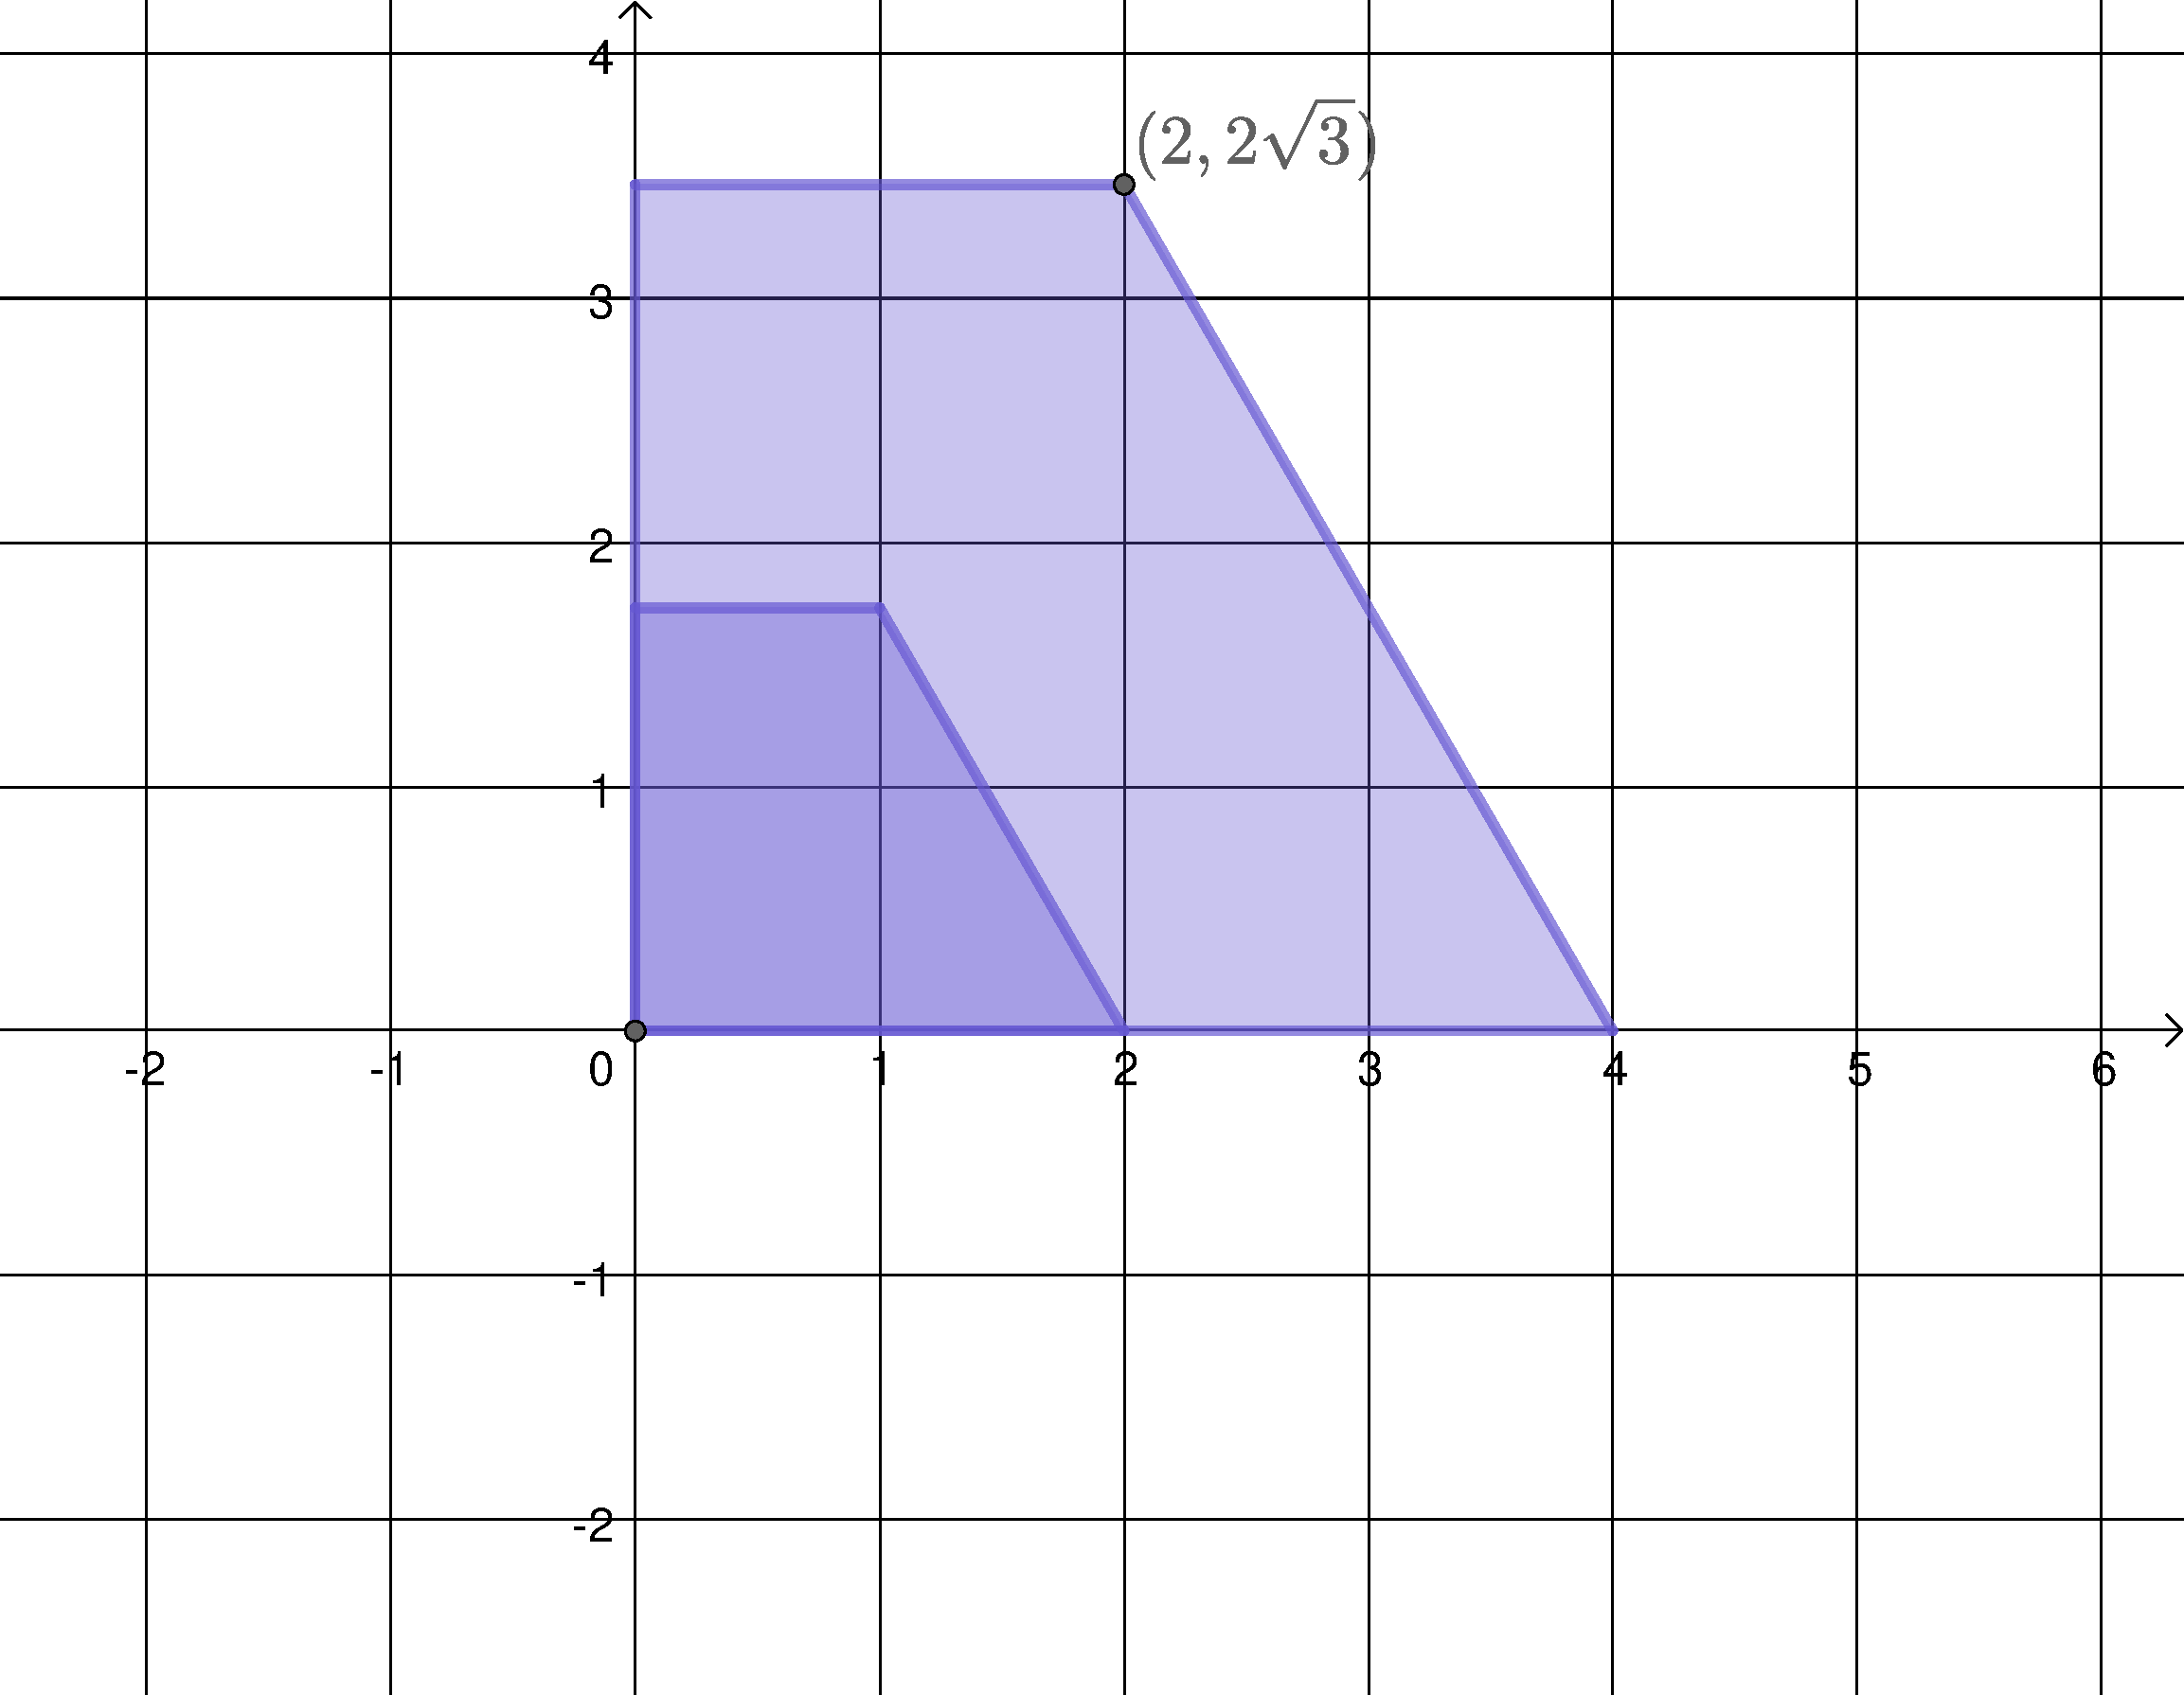
\includegraphics[width=1.75in]{images/rt-trap-scale}}\\
\par\end{center}
So ANOTHER part of the description that defines this rep-tile is \textit{dilate by $\frac12$}.

See if you can find descriptions that turn the whole trapezoid into the remaining parts. You may use
\begin{itemize}
    \item \textbf{Reflection}. Reflection is done about the $x$-axis or about the $y$-axis only.
    \item \textbf{Dilation}. Dilation is done "toward" the origin, $(0,0)$, as seen above. That means the point $(0,0)$ does not move under dilation.
    \item \textbf{Rotation}. Rotation is done \textit{counterclockwise} about the origin, $(0,0)$, as seen above. That means the point $(0,0)$ does not move under rotation and positive angles mean counterclockwise rotation. Use negative angles for clockwise rotation.
    \item \textbf{Translation}. Translation means changing location horizontally and/or vertically and is indicated by an ordered pair, $(\text{horizontal move},\text{vertical move})$ as above.
\end{itemize}
in that order. To help with the exercise, see the interactive GeoGebra page at 
\begin{center}\url{https://www.geogebra.org/m/rswj8az6}.\end{center}
\begin{enumerate}
    \item Write a description that turns the figure on the left (the whole) into the part on the right.\\ \raisebox{-1in}{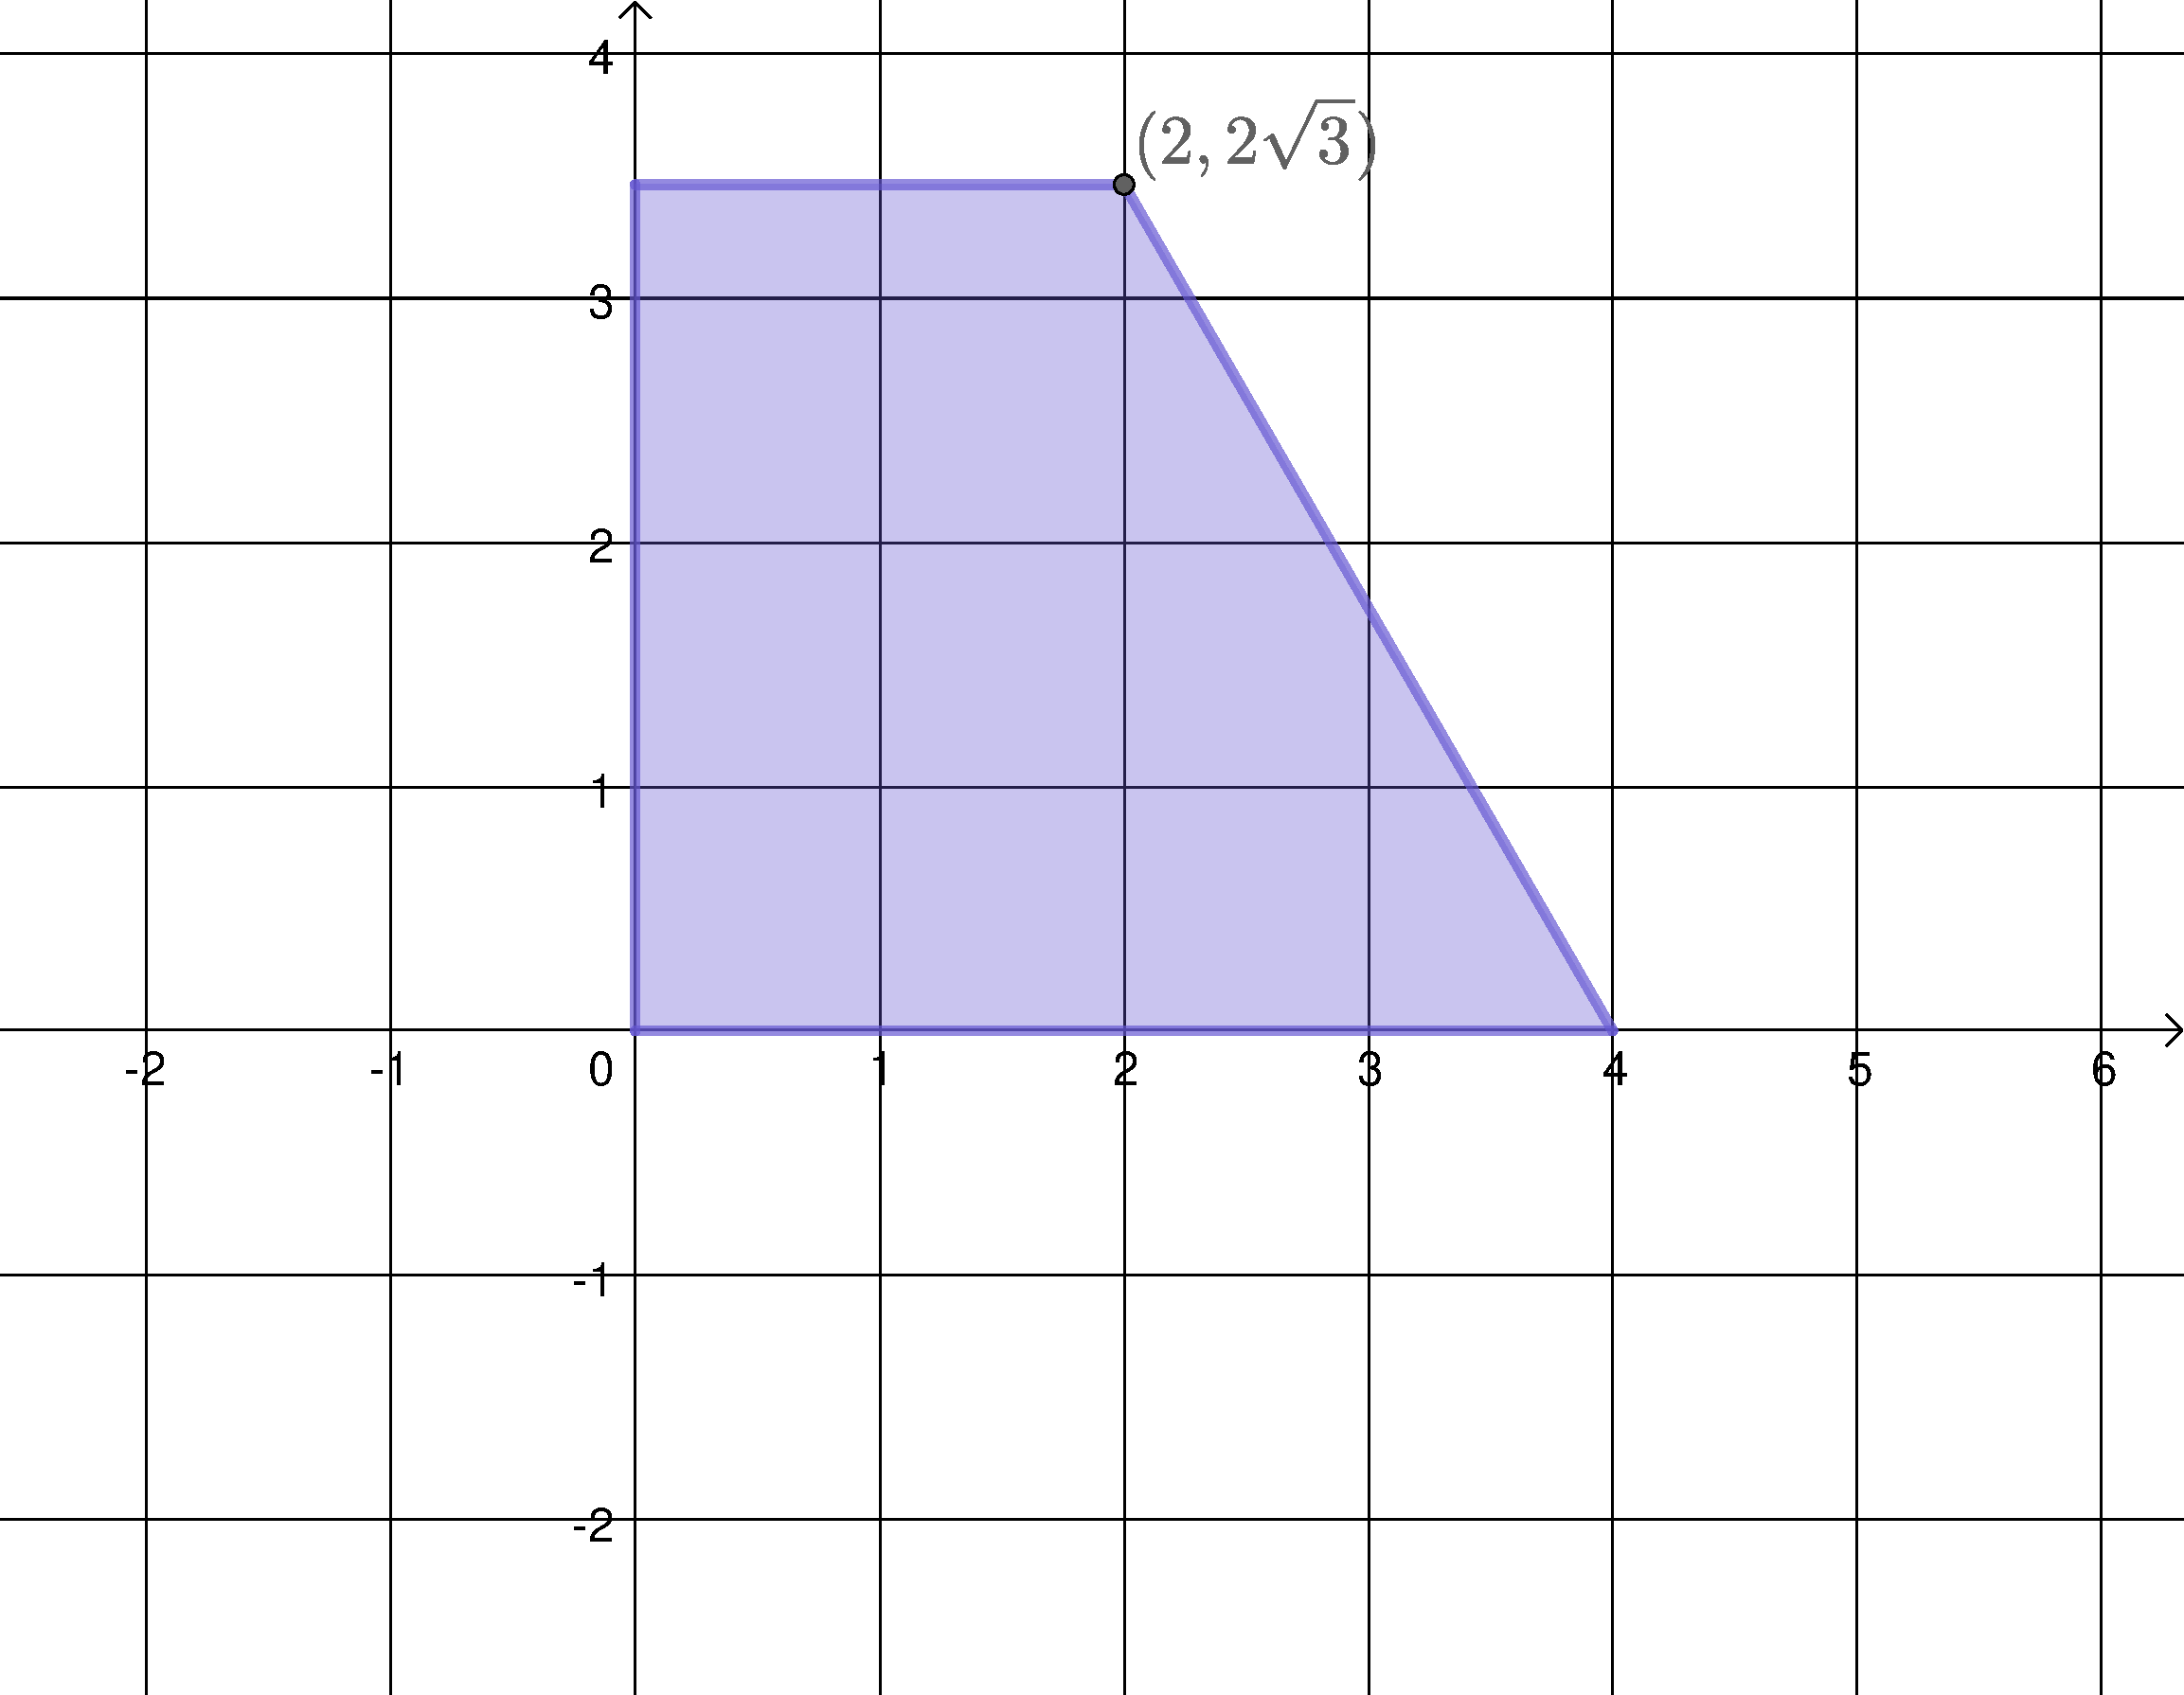
\includegraphics[width=2.5in]{images/rt-trap-start}}\hfill $\longrightarrow$ \hfill \raisebox{-1in}{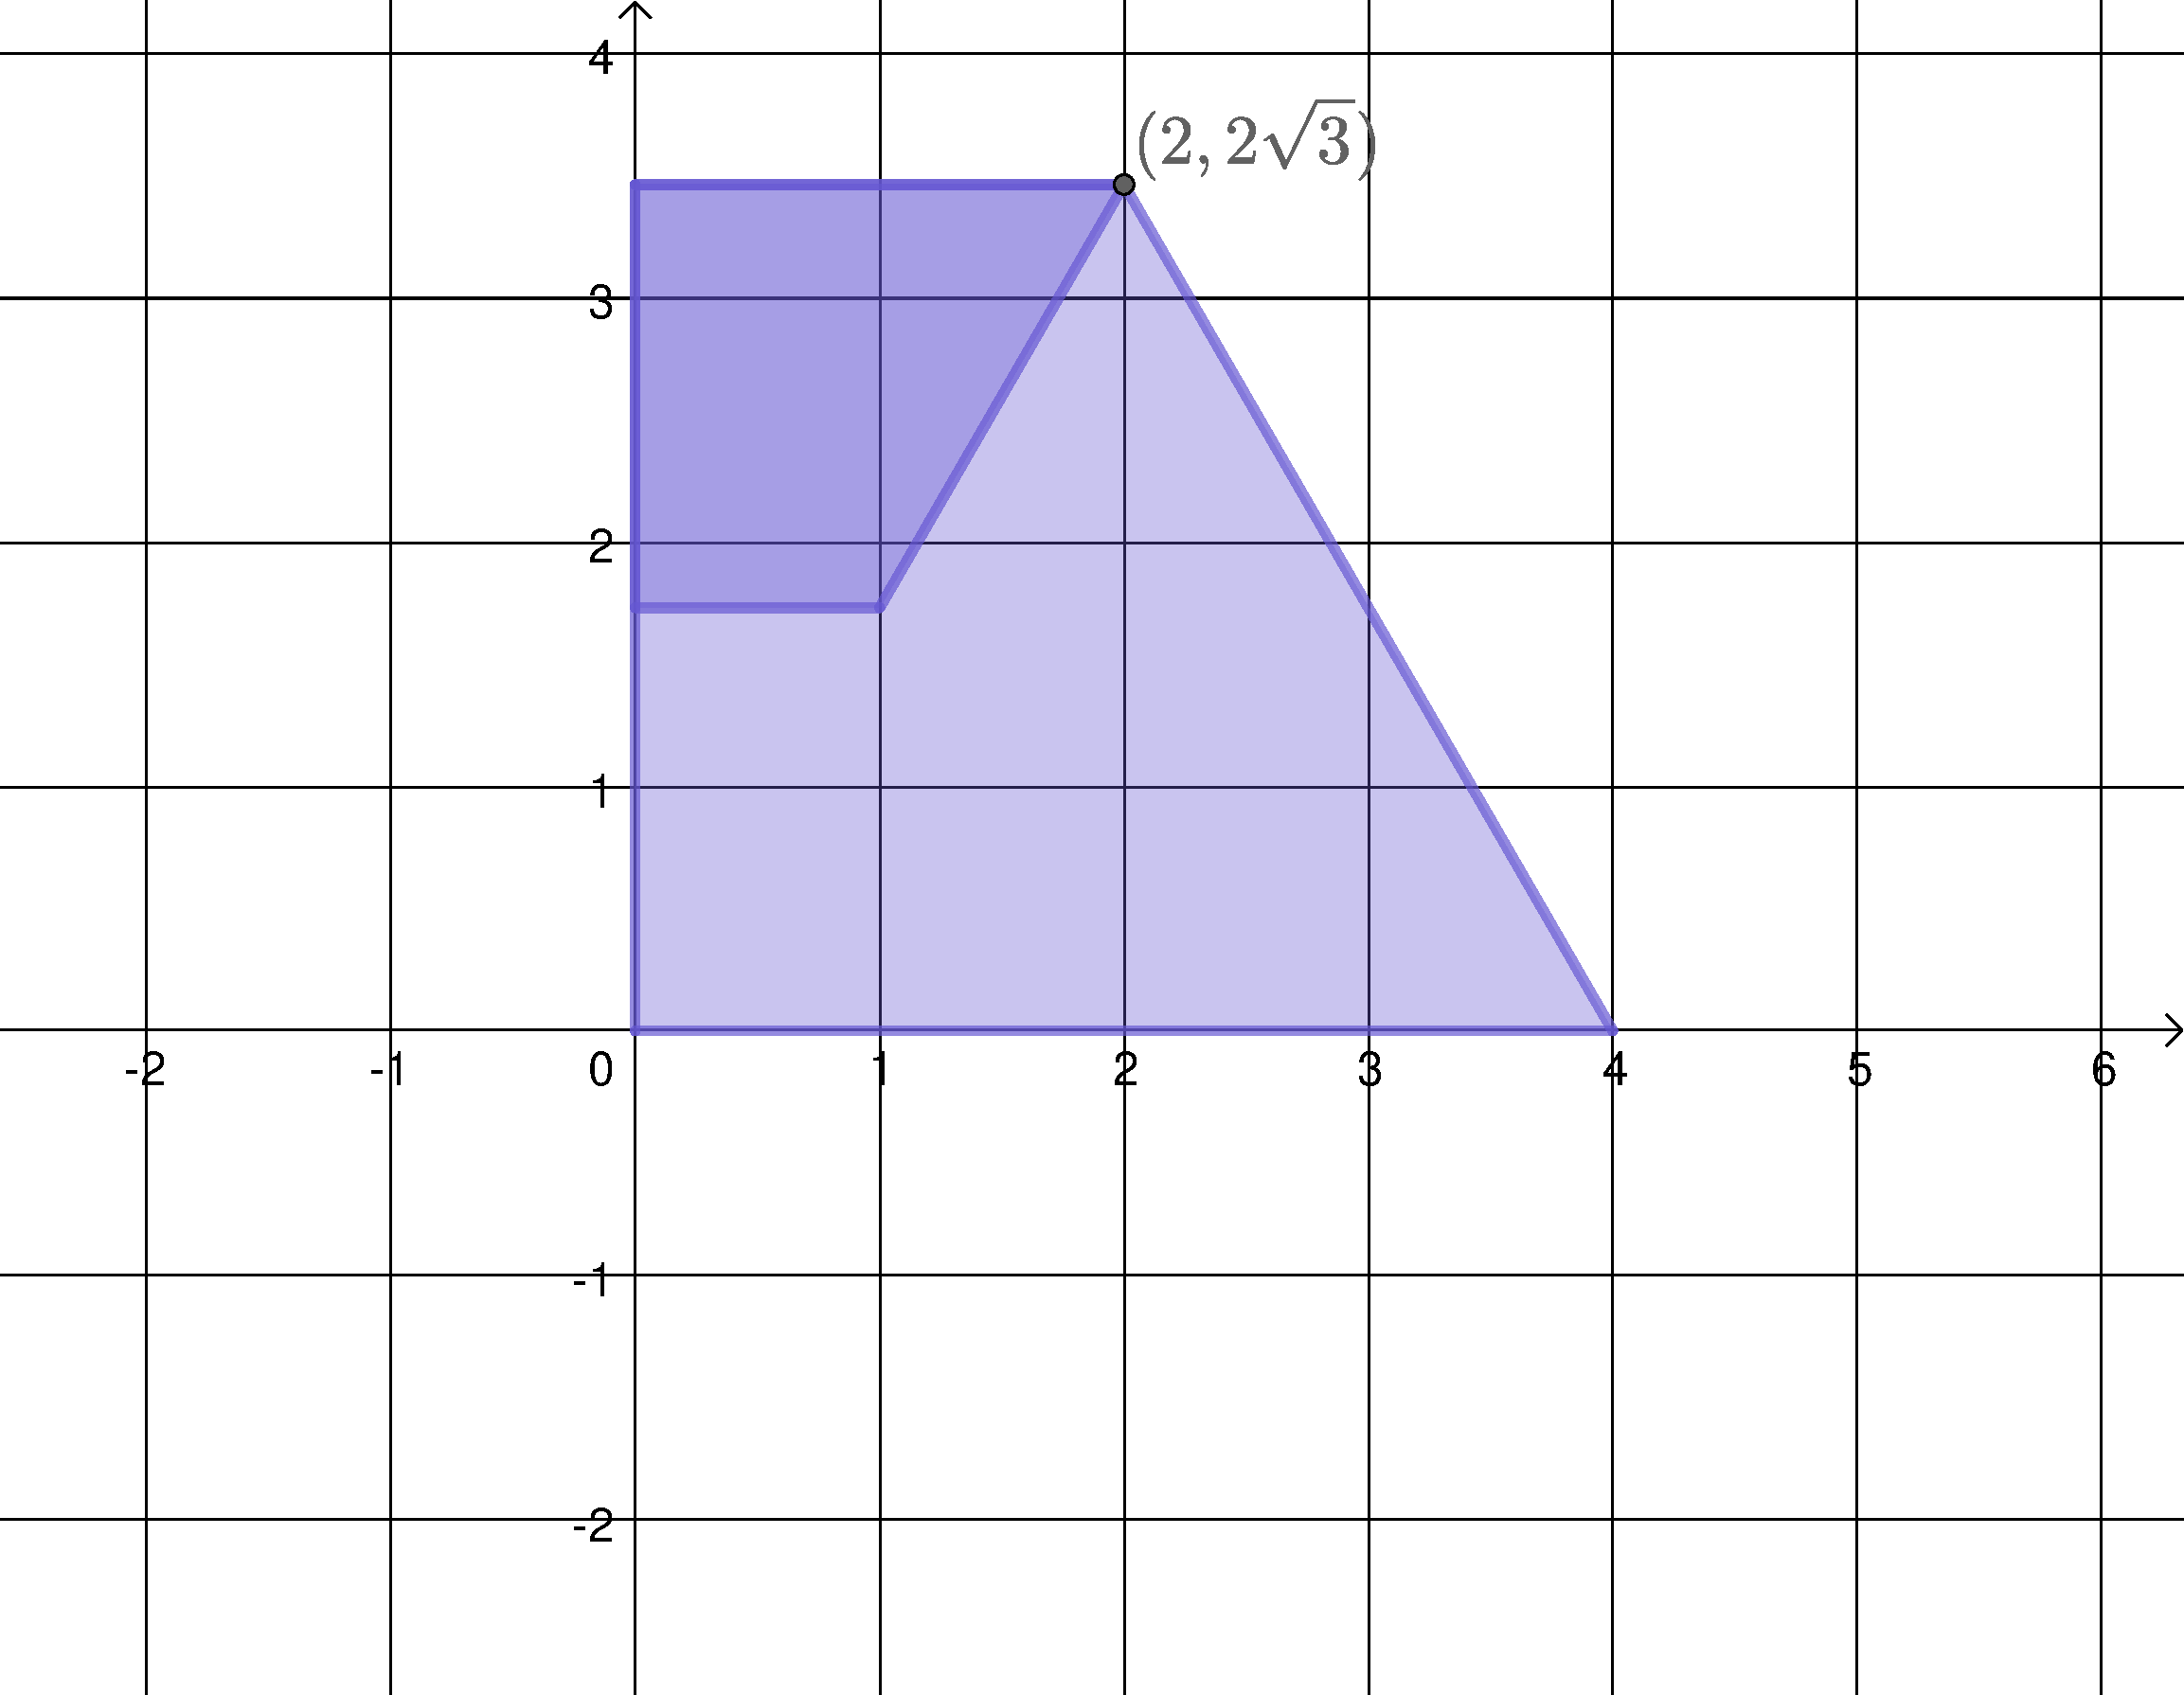
\includegraphics[width=2.5in]{images/rt-trap-part2}}
    \Instr{  \textit{reflect about $x$-axis; dilate by $\frac12$; translate $(3,\sqrt3)$} is one description. There are others, but this one is preferred because it uses the transformations once and in the order listed above. This will be important when entered into the rep-tile designer.}
    \wbnewpage
    \item Write a description that turns the figure on the left (the whole) into the part on the right.\\ \raisebox{-1in}{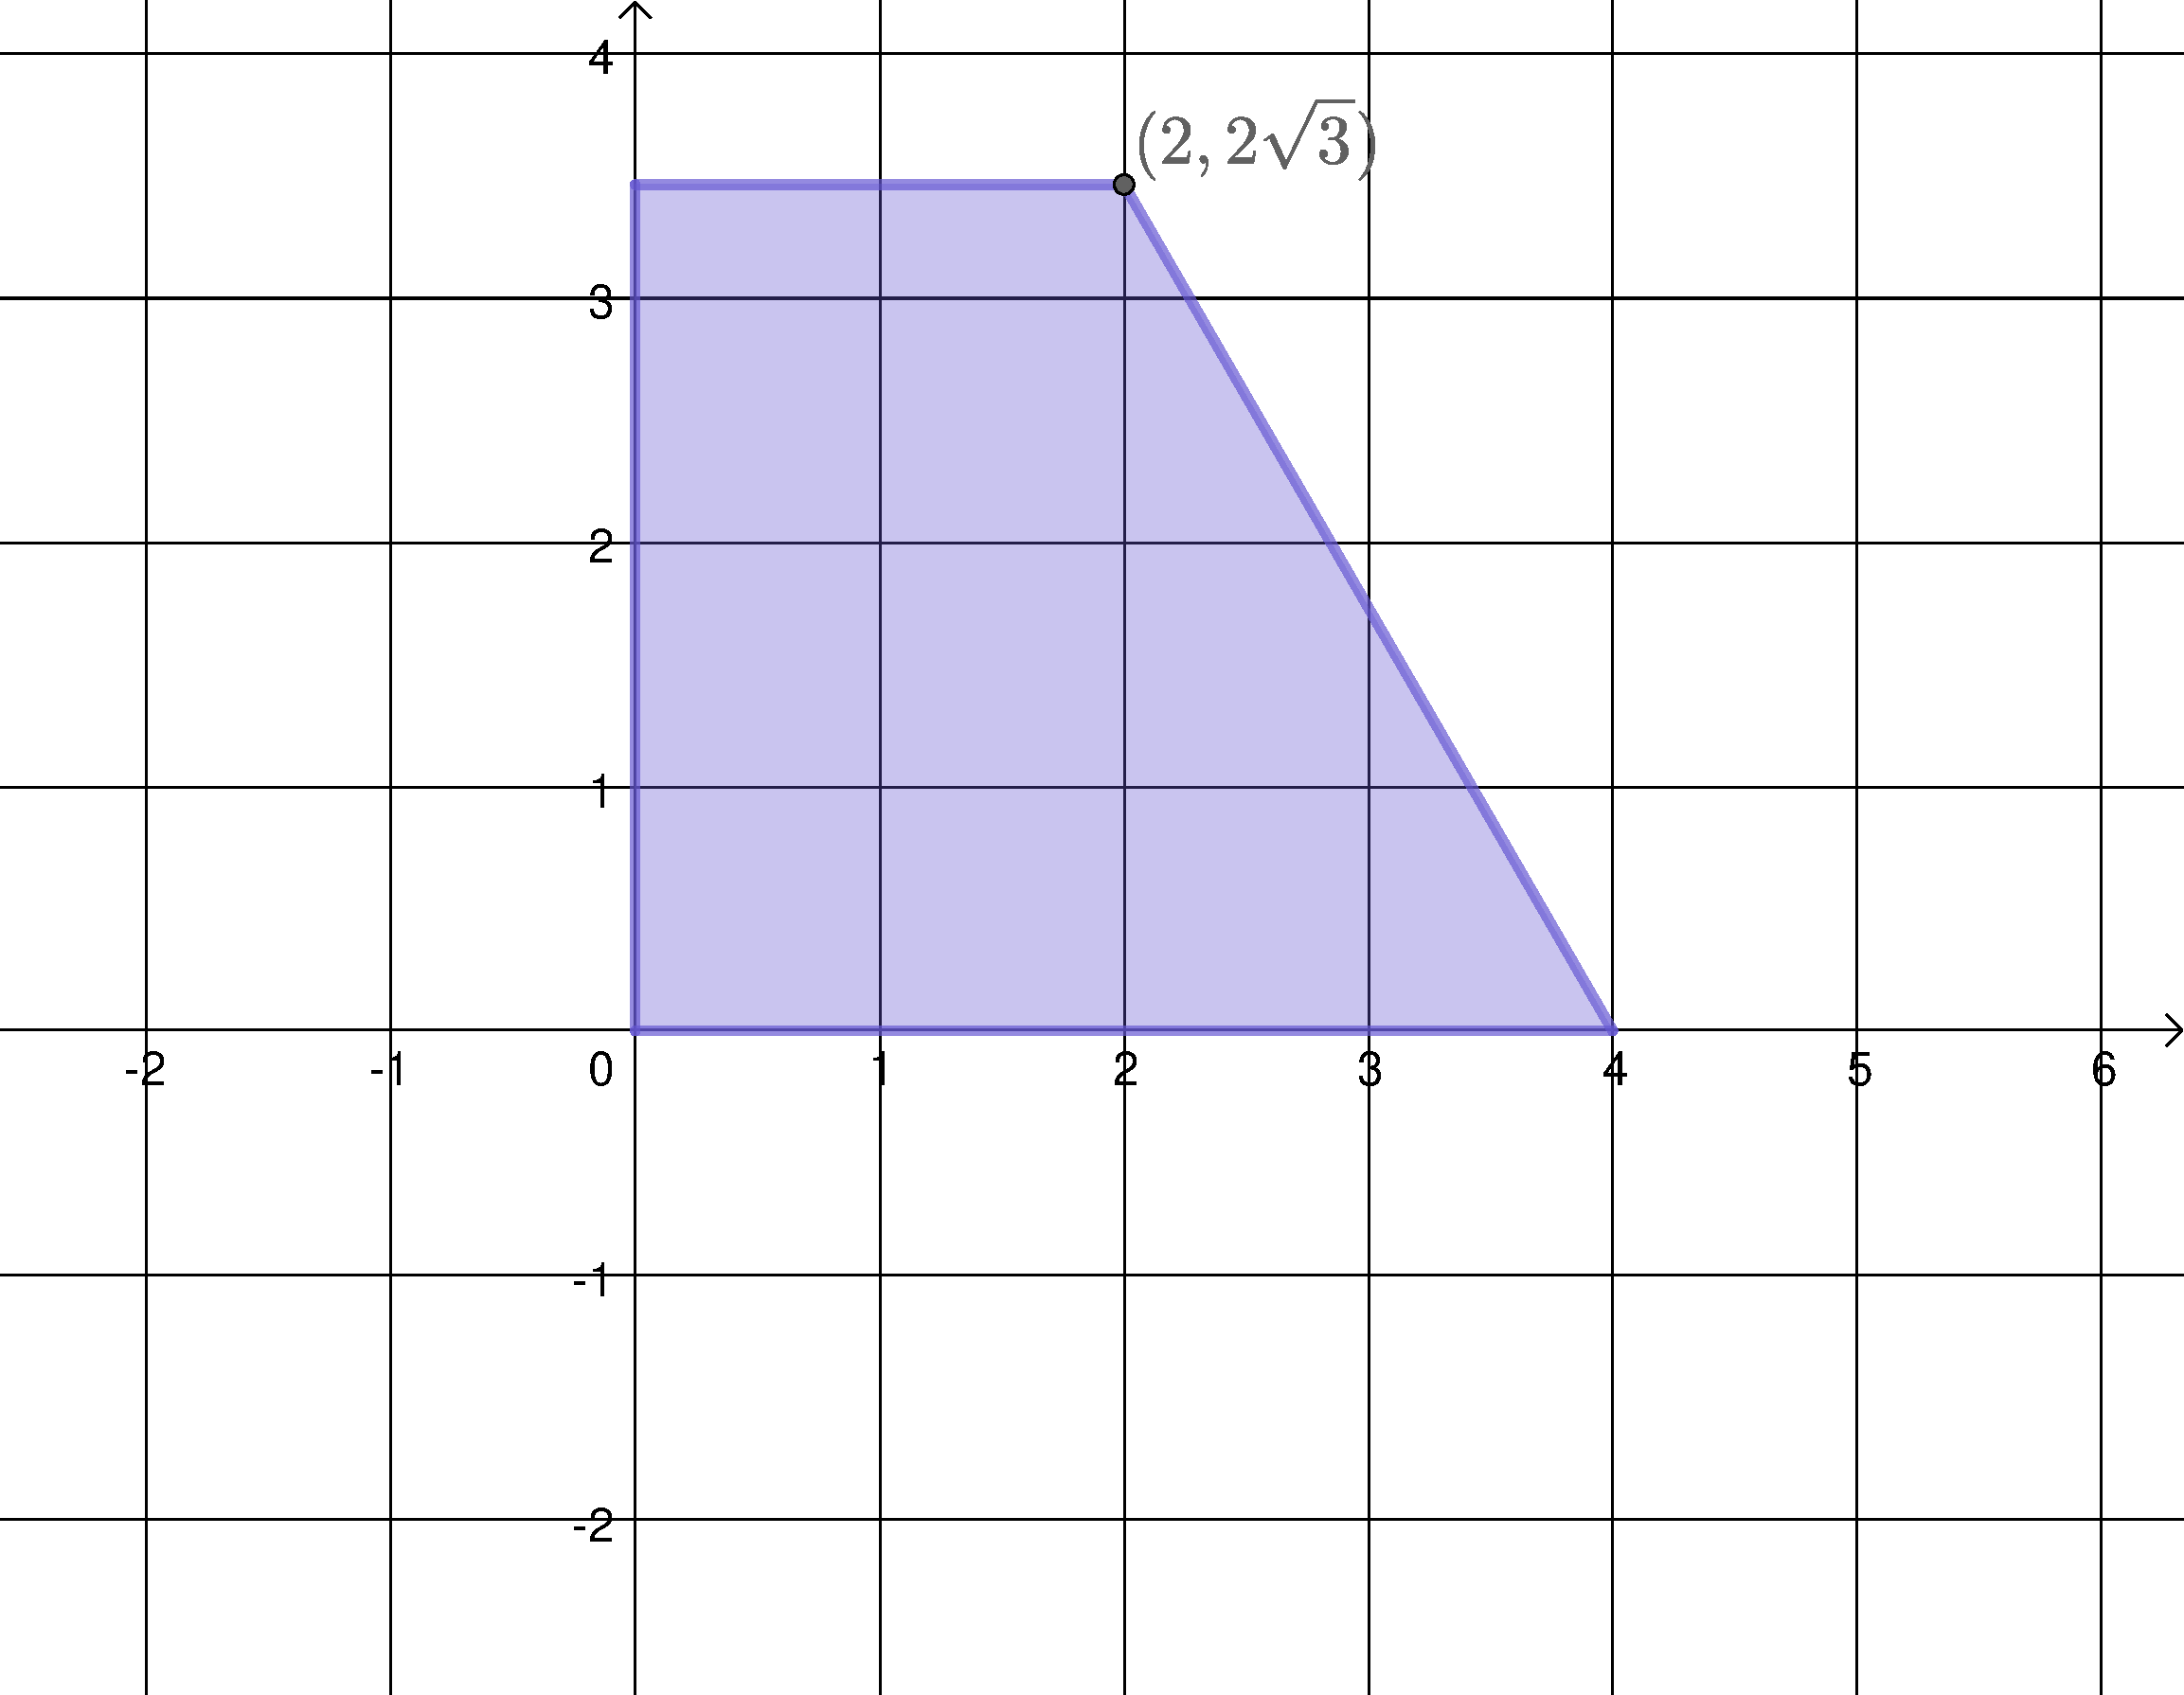
\includegraphics[width=2.5in]{images/rt-trap-start}}\hfill $\longrightarrow$ \hfill \raisebox{-1in}{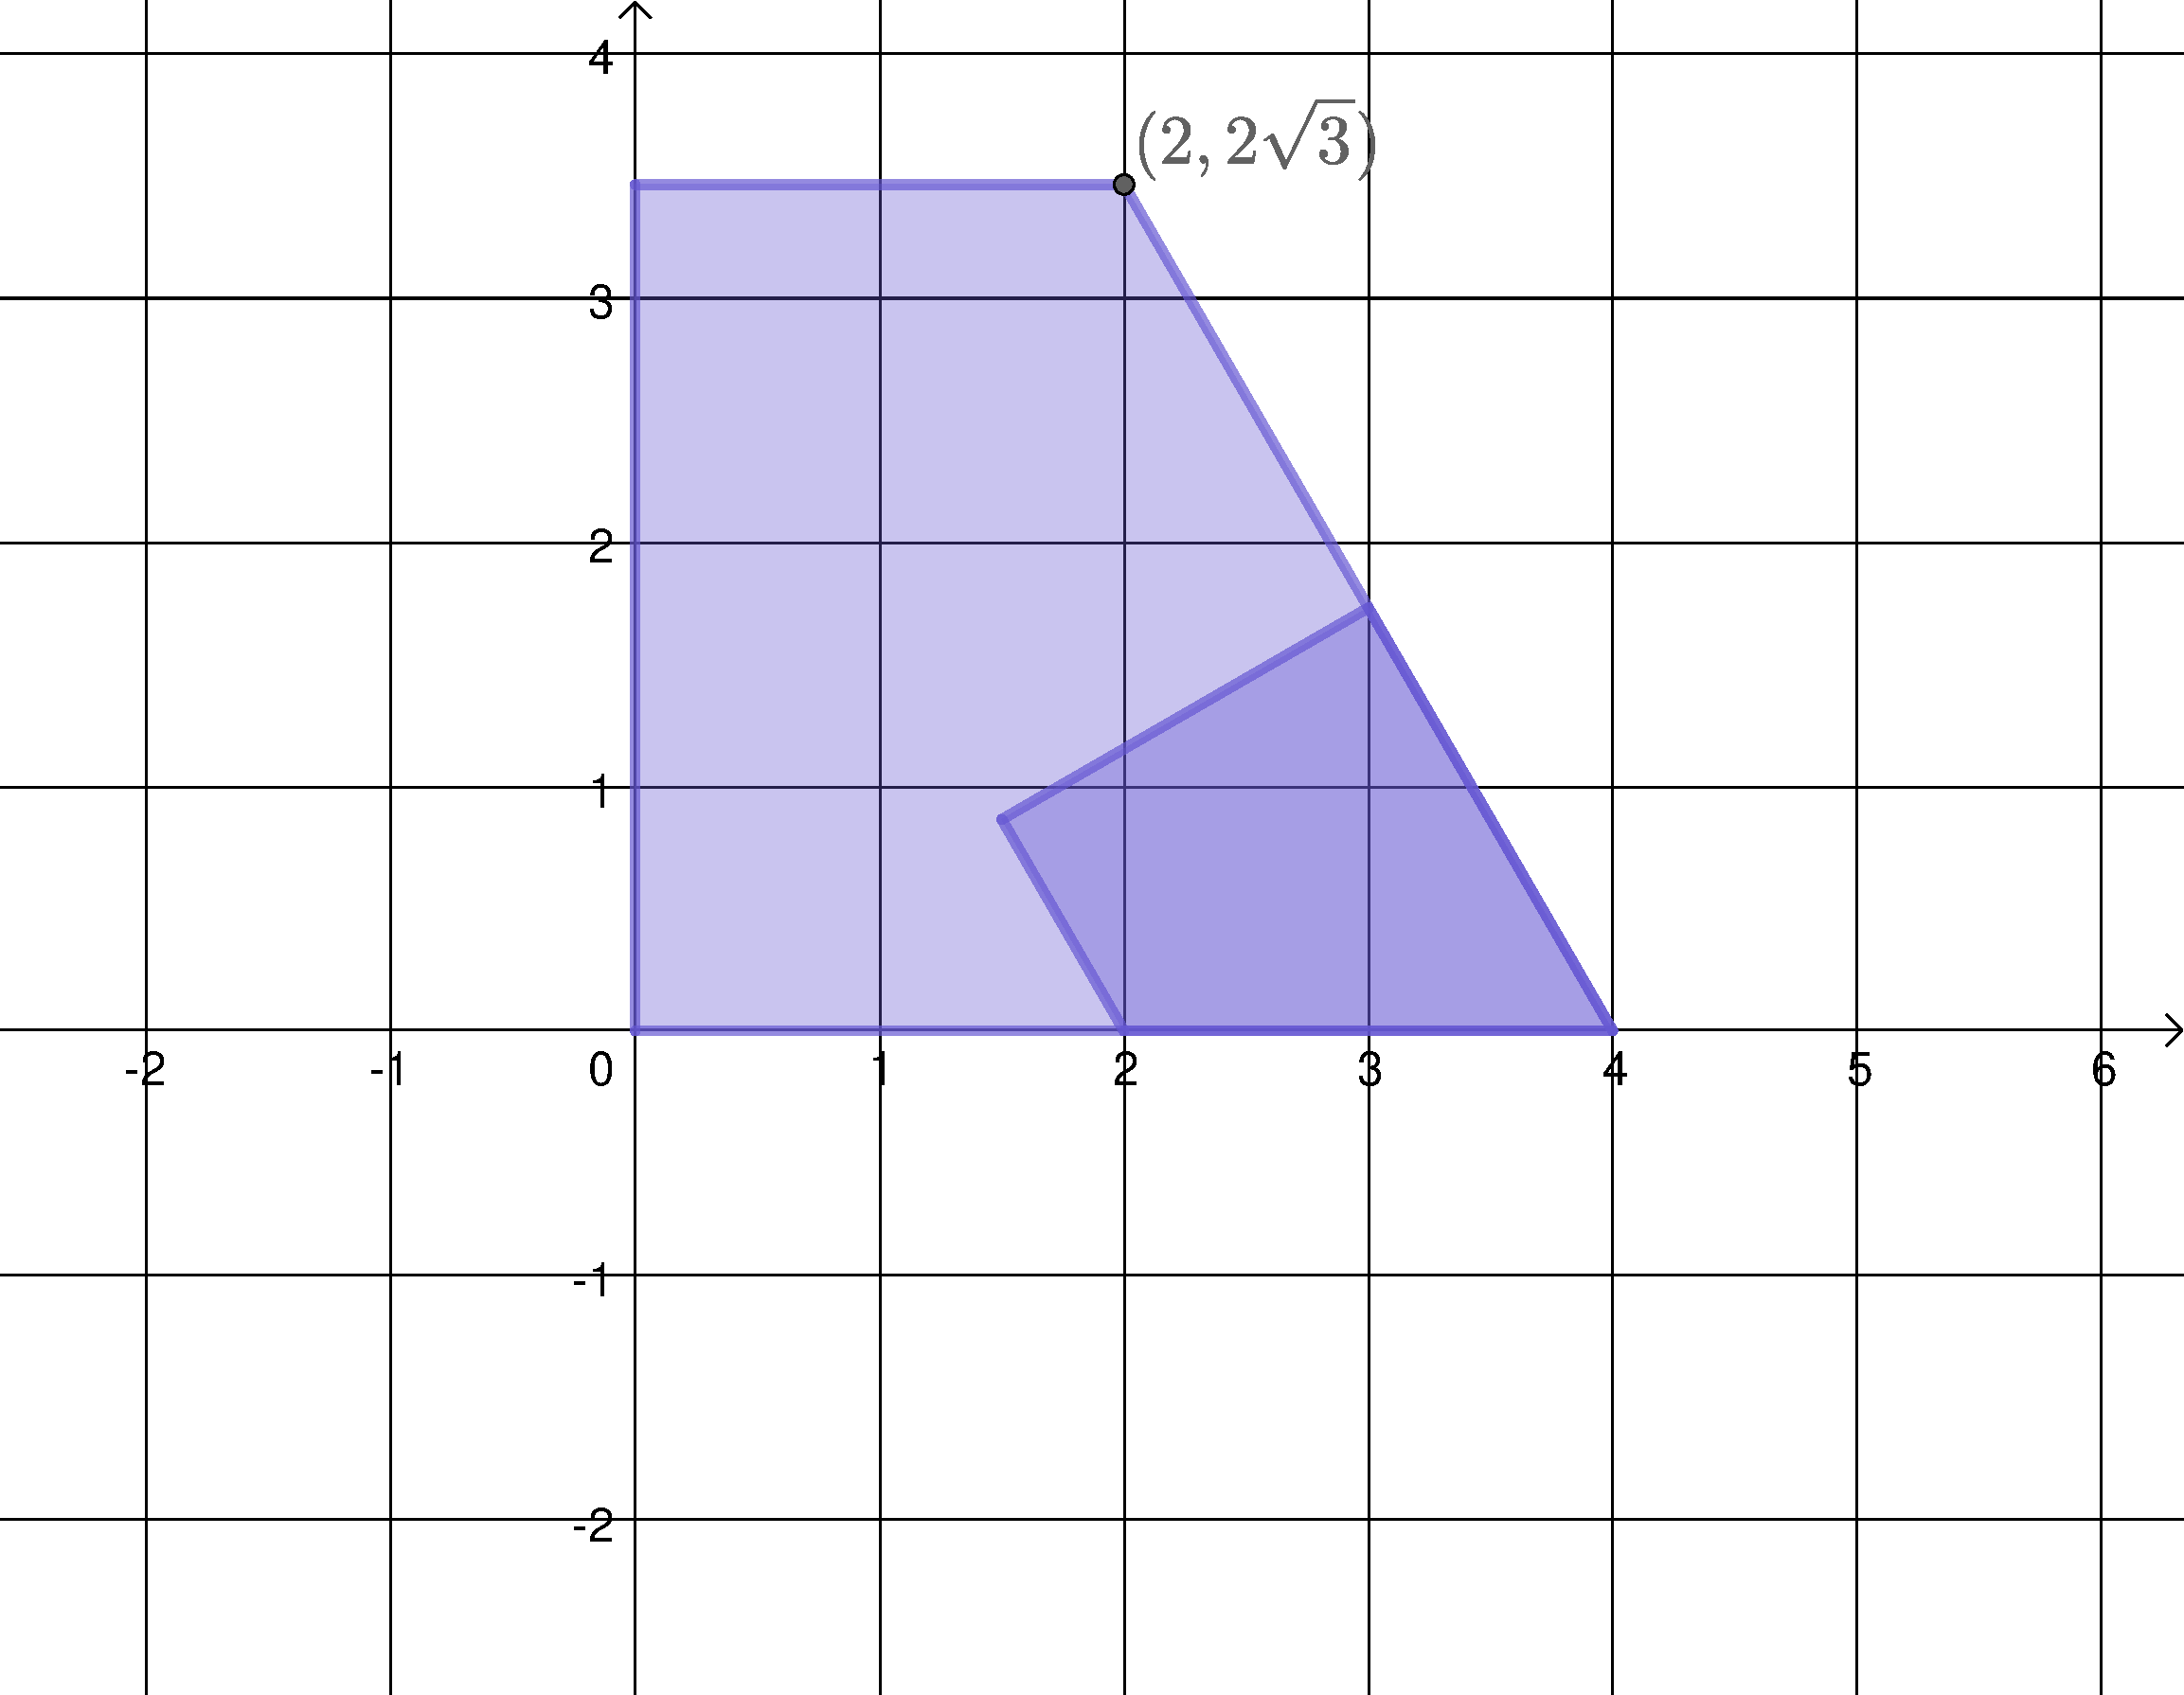
\includegraphics[width=2.5in]{images/rt-trap-part4}}
    \Instr{  \textit{reflect about $x$-axis; dilate by $\frac12$; rotate $-60^\circ$; translate $(3,\sqrt3)$}. \textbf{Students may benefit from cutting out the part, without destroying the handout, and physically moving it through the transformations to make sure they are getting it right. When they have incorrect answers, you can help them see this by physically moving the smaller piece according to their directions and showing them it doesn't end up in the right spot.}}
    \wbvfill
    \item To check that you have the descriptions right
    \begin{enumerate}
		\item Write the FOUR parts of the description of the trapezoid from the introduction and the previous exercises in the table below. The first one is filled in for you.\par
			\setlength{\extrarowheight}{20pt}
			\begin{tabular}{l|c|c|c|c|}
			\multicolumn{1}{l}{} & \multicolumn{1}{c}{Description 1} & \multicolumn{1}{c}{Description 2} & \multicolumn{1}{c}{Description 3} & \multicolumn{1}{c}{Description 4}\tabularnewline
			\cline{2-5} \cline{3-5} \cline{4-5} \cline{5-5} 
			Reflect about & None &  &  & \tabularnewline
			\cline{2-5} \cline{3-5} \cline{4-5} \cline{5-5} 
			Dilate by & 1/2 &  &  & \tabularnewline
			\cline{2-5} \cline{3-5} \cline{4-5} \cline{5-5} 
			Rotate & $120^\circ$ &  &  & \tabularnewline
			\cline{2-5} \cline{3-5} \cline{4-5} \cline{5-5} 
			Translate & $(3,\sqrt 3)$ &  &  & \tabularnewline
			\cline{2-5} \cline{3-5} \cline{4-5} \cline{5-5} 
			\end{tabular}
			\setlength{\extrarowheight}{0pt}
		\item Enter them into the rep-tile designer at \url{https://lqbrin.github.io/tea-time-linear/rep-tile-designer.html}. \par \bigskip\noindent As an example, shown below is the rep-tile designer with descriptions for the parts of the equilateral triangle (as described in the table). A screenshot of this information in Rep-tile Designer appears on the next page.\par
			\begin{tabular}{l|c|c|c|c|}
			\multicolumn{1}{l}{} & \multicolumn{1}{c}{Description 1} & \multicolumn{1}{c}{Description 2} & \multicolumn{1}{c}{Description 3} & \multicolumn{1}{c}{Description 4}\tabularnewline
			\cline{2-5} \cline{3-5} \cline{4-5} \cline{5-5} 
			Reflect about & None & $x$-axis & None & None \tabularnewline
			\cline{2-5} \cline{3-5} \cline{4-5} \cline{5-5} 
			Dilate by & 1/2 & 1/2 & 1/2 & 1/2 \tabularnewline
			\cline{2-5} \cline{3-5} \cline{4-5} \cline{5-5} 
			Rotate & 0 & 0 & 0 & 0 \tabularnewline
			\cline{2-5} \cline{3-5} \cline{4-5} \cline{5-5} 
			Translate & $(0,0)$ & $(1,\sqrt 3)$ & $(2,0)$ & $(1,\sqrt 3)$ \tabularnewline
			\cline{2-5} \cline{3-5} \cline{4-5} \cline{5-5} 
			\end{tabular}
    \begin{center}
        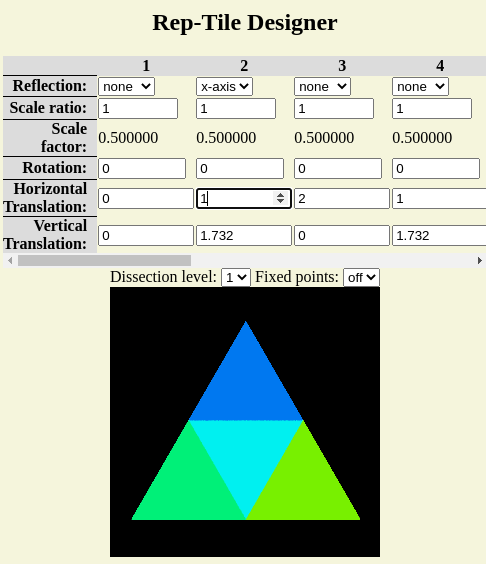
\includegraphics[width=3.7in]{images/rep-tile-designer}
    \end{center}
    Notes:
    \begin{itemize}
        \item You only need to put in the ratio between the sizes of the parts. Rep-tile designer will caclulate the dilation (scale) factors for you.
        \item Select dissection level 1 to see the parts.
    \end{itemize}
    \end{enumerate}
    \item Look at the Rep-tile Designer screenshot below. Can you guess which rep-tile this describes? It is one you have seen before! After you have tried to imagine which one it is, enter the descriptions (as seen in the screenshot below) into Rep-tile Designer to find out. Were you right?
    \begin{center}
        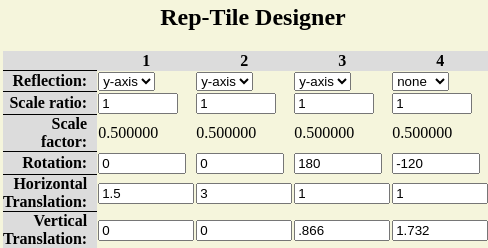
\includegraphics[width=3.7in]{images/rep-tile-mystery}
    \end{center}
    \item Below is an image of an isosceles trapezoid rep-tile from a previous activity. Use the GeoGebra page at \url{https://www.geogebra.org/m/sttrckkz} to help fill in a description for each of the four parts.
	\begin{center}
        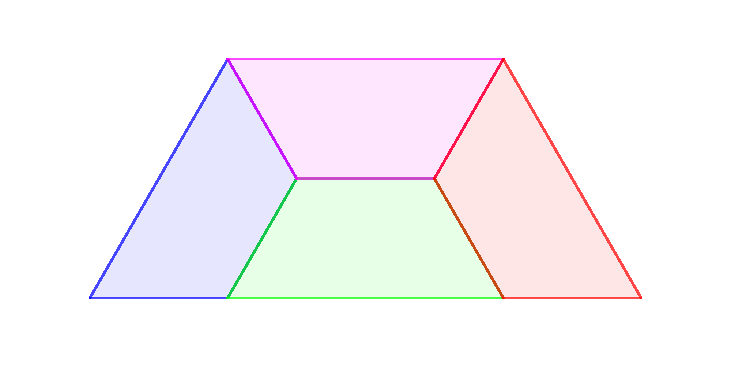
\includegraphics[width=4.2in]{images/Trap-Reptile}
    \end{center}
			\setlength{\extrarowheight}{20pt}
			\begin{tabular}{l|c|c|c|c|}
			\multicolumn{1}{l}{} & \multicolumn{1}{c}{Description 1} & \multicolumn{1}{c}{Description 2} & \multicolumn{1}{c}{Description 3} & \multicolumn{1}{c}{Description 4}\tabularnewline
			\cline{2-5} \cline{3-5} \cline{4-5} \cline{5-5} 
			Reflect about & &  &  & \tabularnewline
			\cline{2-5} \cline{3-5} \cline{4-5} \cline{5-5} 
			Dilate by & &  &  & \tabularnewline
			\cline{2-5} \cline{3-5} \cline{4-5} \cline{5-5} 
			Rotate & &  &  & \tabularnewline
			\cline{2-5} \cline{3-5} \cline{4-5} \cline{5-5} 
			Translate &  &  &  & \tabularnewline
			\cline{2-5} \cline{3-5} \cline{4-5} \cline{5-5} 
			\end{tabular}
			\setlength{\extrarowheight}{0pt}

\end{enumerate}

\wbnewpage

\subsection{Exit Slip: Create your own}

Below is an image of a trapezoid rep-tile you have not seen before. Use the GeoGebra page at \url{https://www.geogebra.org/m/hzkuwzex} to help fill in a description for each of the four parts.
	\begin{center}
        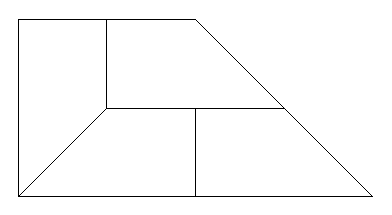
\includegraphics[width=4.2in]{images/langford-05}
    \end{center}
			\setlength{\extrarowheight}{20pt}
			\begin{tabular}{l|c|c|c|c|}
			\multicolumn{1}{l}{} & \multicolumn{1}{c}{Description 1} & \multicolumn{1}{c}{Description 2} & \multicolumn{1}{c}{Description 3} & \multicolumn{1}{c}{Description 4}\tabularnewline
			\cline{2-5} \cline{3-5} \cline{4-5} \cline{5-5} 
			Reflect about & &  &  & \tabularnewline
			\cline{2-5} \cline{3-5} \cline{4-5} \cline{5-5} 
			Dilate by & &  &  & \tabularnewline
			\cline{2-5} \cline{3-5} \cline{4-5} \cline{5-5} 
			Rotate & &  &  & \tabularnewline
			\cline{2-5} \cline{3-5} \cline{4-5} \cline{5-5} 
			Translate &  &  &  & \tabularnewline
			\cline{2-5} \cline{3-5} \cline{4-5} \cline{5-5} 
			\end{tabular}
			\setlength{\extrarowheight}{0pt}
			
	\vspace{15pt}
	\noindent Enter your descriptions in the Rep-tile Designer at
	\begin{center}
		\url{https://lqbrin.github.io/tea-time-linear/rep-tile-designer.html}
	\end{center}
	to check your answers. 

\newpage


% New Section %%%%%%%%%%%%%%%%%%%%%%%%%%%%%%%%%%%%%%%%%%%%%%%%
\section{Funny Dice}\label{sec:FunnyDice}
%%%%%%%%%%%%%%%%%%%%%%%%%%%%%%%%%%%%%%%%%%%%%%%%%%%%%%%%%%%%%%
\wbnewpage
%%%%%%%%%%%%%%%%%%%%%%%%%%%%%%%%%%%%%%%%%%%%%%%%%%%%%%%%%%%%%%
\subsection{Entrance Activity: Dice}

\Instr{  Make sure to bring sufficient copies of the handout ``D4.pdf'' and enough scissors to go around for this activity.}

Dice are certainly familiar items from the world around us.  There are games that can be played with dice alone, and there are many games that use dice to add an element of randomness -- for instance in Monopoly, each player rolls the dice when it's their turn and that determines how many positions their token moves.  A single die is a random number generator with possible values from 1 to 6.

\centerline{\includegraphics[scale=.1]{images/dice.jpg}}

Often (when numbers larger than 6 are required), we use two die.  That gets us numbers from 2 to 12, but there's a funny consequence -- some numbers are more likely to come up than others.

There are 6 different ways that you can roll a 7 with two die.  Can you list them?

\

\centerline{ \begin{tabular}{c|c} 
\bigstrut die 1 & die 2 \\ \hline
\bigstrut & \\ \hline
\bigstrut & \\ \hline
\bigstrut & \\ \hline
\bigstrut & \\ \hline
\bigstrut & \\ \hline
\bigstrut & \\ 
\end{tabular}
}
\bigskip

How many ways can you roll an 11?

\wbvfill

So in a game played with rolling two dice, do you expect to see more  7's or more 11's throughout the game?

\wbvfill


\wbnewpage

\subsection{Activity: Plaited Models}
If we want ``dice-like things'' (random number generators that give equal weight to the options) we'll need solid geometric objects that are nice and regular, but that have different numbers of sides.  Here are a few examples:

\centerline{\includegraphics[scale=.1]{images/fancy_dice.jpg}}
\bigskip

There are other options, but a good place to start is shapes that have all the same regular polygon as their sides. These are called Platonic solids, named after the greek philosopher Plato. The smallest platonic solid is known as a tetrahedron -- gamers call it D4. The pyramids that can be found in Egypt and a few other places around the world have triangular sides, but square bases.  Can you imagine what it would look like if a pyramid's base was also a triangle?

\bigskip

In this activity, we will make models of a D4 and a cube using ``strips of paper'' woven together. This technique is called plaited models of $3$D- solids.
\begin{enumerate}
\item Cut out each image provided into intact strips only on the solid black lines.
\item All dotted edges indicate a line to be folded during the construction. 
\item The pips (dots) indicate the shapes (faces) that will be showing on the outside of the shape
\item All blank shapes will be woven under another piece of paper when completed.
\end{enumerate}

\newpage

\centerline{\includegraphics[scale=1.75]{images/PlaitedD4.eps}}

\newpage

\centerline{\includegraphics[scale=1.65]{images/PlaitedDice.eps}}



\newpage

\subsection{Activity: Why Only Five?}
The shapes called Platonic solids are 3 dimensional shapes that have each side being the exact same 2 dimensional shape and they are regular, meaning all the angles are the same measurement and the sides are the same length.. These 2D shapes are called the faces of the 3D shape.\Instr{  Refrain from using the terms "planar graph" or "Euler characteristic" while working on the Platonic solids. These terms have a tendency to lead students to do a research paper on the WND on a doughnut project rather than any problem solving."}
\begin{enumerate}

\item Let's start with the D4. Notice that there are 3 edges on each triangle (duh!) and since there are 4 triangles that makes a total of $3 \cdot 4 \; = \; 12$ edges.  But there are only 6 edges on the D4 we just made.  Can you explain why?


\Instr{  In the ``images'' directory are pdfs of templates for constructing an icosahedron and a dodecahedron.  If this activity stretches over two class periods there may be time for students to actually construct them, and hence it might be nice to bring a supply of copies of the templates (ideally on heavier paper) and scissors and glue. }

\wbvfill



\item Think a bit about why cubes are the perfect 3-d shape to use for dice.  Cubes are made up of squares, but you could make an imperfect cube out of rectangles -- think of a brick.  Explain why tossing a brick would be a poor choice for generating random numbers.
\end{enumerate}
\wbvfill

\wbnewpage
It seems we should build our ``fancy'' dice using faces that are {\bf regular} like a square.  The regular polygons that can be used are:

\begin{enumerate}
    \item equilateral triangles
    \item squares
    \item regular pentagons
\end{enumerate}

Of course, triangles are the smallest possible polygons, but what about shapes with more sides?  Can you come up with a reason why we couldn't make a 3-d object with regular hexagons, heptagons, octagons? (If you have physical objects like these, try to build a 3-d object, what happens?)

\wbvfill

\wbnewpage

A tool we can use to think carefully about polyhedra (that's the generic term for a solid with many sides) is the so-called {\em net} of the polyhedron.  There are generally many different nets for a given polyhedron.  Here's one for a cube:
\bigskip

\centerline{\includegraphics[scale=.25]{images/cube-net.png}}

Officially, a net wouldn't include the little tabs that are meant for gluing the model together. But, as you can probably tell from the example, the net of a solid is a flat template that can be folded up to cover the exterior of the solid.

Which of the following is a net for the tetrahedron? (Cut them out and see!)
\bigskip

\centerline{\includegraphics[scale=.25]{images/tetrahedron_nets.png}}
\wbnewpage

A quicker way to rule out a potential net is to count how many polygons will meet at each corner.  In a tetrahedron, exactly $3$ triangles meet at each corner. Now do you see which one of the above is impossible?

\wbvfill

Let's recap for a minute.  We're trying to figure out how to make ``fancy'' dice that will have a different number of sides than a cube does.  We know that the faces of our dice will have 3, 4, or 5 sides.  Finally, it seems that the number of faces that meet at a corner is important.  Some of you may know about D8, D12 and D20, but the only solids we've discovered together so far are D4 and D6 -- the tetrahedron and the cube.

Let's collect what we've found so far in a table.

Also, let's (please!) agree to use the following abbreviations:

$F =$ the number of faces on the object.

$C =$ the number of corners on the object.

$F/C =$ the number of faces that meet at a corner.

$C/F =$ the number of corners on each face.

$E =$ the number of edges.
\bigskip

\begin{tabular}{r|c|c|c|c|c} 
\bigstrut name & $F$ & $C$ & $F/C$ & $C/F$ & $E$ \\ \hline
\bigstrut tetrahedron & \hstrut & \hstrut & \hstrut & \hstrut & \hstrut \\ \hline
\bigstrut cube & & & & & 
\end{tabular}

\wbvfill

\wbnewpage

Near the beginning of this activity we asked, ``Can anyone come up with a reason why we couldn't make a 3-d object with hexagons, heptagons, octagons, etc. as the sides?''  There are two facts that explain the situation.

\begin{itemize}
    \item[{\bf Fact 1:}] You have to have 3 or more faces meeting at a corner. \newline
    (What would it look like if only two faces (of whatever type (sorry about the nested parentheses)) met at a corner?)
    \item[{\bf Fact 2:}] The sum of the angles on the faces that meet at a corner must be less than $360^\circ$ \newline
\end{itemize}

Fact 2 might best be illustrated by an example.  What would it look like, if instead of having 3 squares meet at a corner, we tried to get 4 squares to meet at a corner. (Hint: look down.)

The angle on the corner of a hexagon is $120^\circ$ and if $3$ of them met at a corner, we'd get a tiling of the plane -- not a polyhedron of any sort.  Here's a hard question: what is the angle found on the corner of a regular pentagon, and how many regular pentagons could meet at the corners of a polyhedron?

\vspace{1in}

Alright then! If a polyhedron has squares as its faces there must be \underline{\hstrut} of them meeting at a corner, and that gets us a cube!  If a polyhedron has regular pentagons as its faces there must also be \underline{\hstrut} of them meeting at a corner, and that beast is called the dodecahedron.  We'll come back to that!

What are the possible values of $F/C$ if the faces are triangles?

\vspace{.5in} 

\wbnewpage

Here's a bit more of the table we started previously. The new object in the row that's been added is called the {\em octahedron} and the entries that are pre-filled tell us that it's made of triangles with 4 of them meeting at a corner. A little thinking about etymology will probably let you guess how many faces it has.  Rather than building a model, we'll just try to get you to visualize this solid in your mind's eye.  Imagine taking two (Egyptian-style, square based) pyramids and gluing them together along their square bases -- the resulting thing would only have triangles (8 of them!) visible on the outside and there would be $4$ meeting at each corner.

With that visualization you should now be able to fill out the remaining entries in the octahedron row.

\

\setlength{\tabcolsep}{18pt}
\begin{tabular}{r|c|c|c|c|c} 
\bigstrut name        & $F$ & $C$ & $F/C$ & $C/F$ & $E$ \\ \hline
\bigstrut tetrahedron & 4   & 4   & 3     & 3     & 6 \\ \hline
\bigstrut cube        & 6   & 8   & 3     & 4     & 12 \\ \hline
\bigstrut octahedron  &     &     & 4     & 3     &   \\
\end{tabular}
\bigskip



\Instr{  It's possible that students might ask about gluing tetrahedra together in a similar fashion.  Of course that gets us 6 faces, and we've already got cubes\textellipsis Ask them about regularity - does the solid formed out of two triangular pyramids glued together at their bases have the same number of faces meeting at each corner?  This inquiry also leads to the interesting family of bi-pyramidal dice.}

\wbnewpage

There are two remaining objects in this list of the $5$ Platonic solids we're trying to build.
The {\em dodecahedron} (aka D12) and the {\em icosahedron} (aka D20).  One of them is built of 5-sided polygons meeting 3 at a corner.  The other is made of 3-sided polygons meeting 5 at a corner.  Isn't that weird switching-around of 3's and 5's interesting?

Here's a net for the dodecahedron:
\bigskip

\centerline{\includegraphics[scale=.5]{images/dodecahedron_template.pdf}}
\bigskip

\newpage

This is a net for the icosahedron:
\bigskip

\centerline{\includegraphics[scale=.5]{images/icosahedron_template.pdf}}
\bigskip

\newpage

You guessed it! It's time to completely finish the table!
\bigskip


\setlength{\tabcolsep}{18pt}
\begin{tabular}{r|c|c|c|c|c} 
\bigstrut name        & $F$ & $C$ & $F/C$ & $C/F$ & $E$ \\ \hline
\bigstrut tetrahedron & 4   & 4   & 3     & 3     & 6  \\ \hline
\bigstrut cube        & 6   & 8   & 3     & 4     & 12 \\ \hline
\bigstrut octahedron  & 8   & 6   & 4     & 3     & 12 \\ \hline
\bigstrut dodecahedron&     &     &       &       &    \\ \hline
\bigstrut icosahedron &     &     &       &       &    \\ \hline
\end{tabular}
\bigskip

Look carefully at your completed table.  Search for patterns.  Remember that weird switching around of 3's and 5's?  Mathematicians say that ``the tetrahedron is self-dual and the other platonic solids can be divided into pairs that are dual to one another.''  Any idea what they're talking about?

\newpage

\subsection{Exit Slip}

\begin{enumerate}
    \item What would you guess the Greek prefix {\em icosa} means?
    
    \wbvfill
    
    \item The word ``dozen'' literally means $2+10$.  How is this silly fact relevant to the naming of Platonic solids?
 
     \wbvfill
       
    \item Let's try some multi-counting.  Every one of the pentagons on a dodecahedron has 5 corners, and since there are 12 pentagonal faces that makes for $12 \cdot 5 \; = \; 60$ corners.  By what factor did we over-count the corners? \underline{\hstrut}
    
    How many corners are actually on a dodecahedron? \underline{\hstrut}

    \wbvfill
        
    \item Every face of a cube has 4 corners .  Since there are 6 faces on a cube, we get 
    $6 \cdot 4 = 24$ corners.  By what factor did we over-count the corners? \underline{\hstrut}
    
    How many corners are actually on a cube? \underline{\hstrut}
    
    \wbvfill
    
\end{enumerate}

\newpage

\subsection{Duals}

Look at the final table in the previous activity, and notice that there are some weird coincidences in the numbers.  For example, the dodecahedron and the icosahedron have the number of faces and the number of corners interchanged.  These coincidences lead to the idea of {\em duality}.

Which pairs of Platonic solids are dual to one another?

\wbvfill

Why is the tetrahedron called self-dual?

\wbvfill

You can make drawings of the platonic solids that lie flat in the plane, using some ideas from the mathematical area known as Topology.
(Topology means the study of shape.  Topologists study the things that remain the same even when an object is deformed somewhat.)

Imagine making a Platonic solid out of spaghetti noodles (maybe with meatballs holding the corners together).  Then (very carefully) cook your solid until the noodles get noodly. You should now be able to lay your ``solid'' out flat in the plane in such a way that no noodles cross each other.

Here's a wet noodle diagram of a cube:

\centerline{\includegraphics[scale=.5]{images/wet_noodle_cube.png}}

\wbnewpage

\begin{enumerate}
    \item Make wet noodle diagrams of all 5 platonic solids.
    
    \wbvfill
    
    \item The corners of your Platonic solid are the points (meatballs) in the wet noodle diagram.  The edges of the solid are the noodles.  The faces of the Platonic solid have become regions in the plane surrounded/bordered by noodles.  Count the regions in each of your 5 noodle diagrams.
    
    \vspace{1in}
    
    \wbnewpage
    
    \item What happened to the missing faces?
    
    \wbvfill
    
    \item There is a process known as {\em truncation} that essentially means ``cut off the corners.''  Draw a wet noodle diagram for a truncated cube:
    
    \centerline{\includegraphics[scale=.25]{images/TruncatedCube.jpeg}}
    
    \wbvfill
    
    \item Now try making a wet noodle diagram for a truncated tetrahedron.
    
    \wbvfill
    
    \wbnewpage
    
    \item Try a wet noodle diagram of a 5-sided pyramid.
    
    \wbvfill
    
    \item Let's do some counting!  How many regions, edges and vertices (the fancy way to say `corners') are there in each of your diagrams?
    \bigskip
    
    Count the region outside your diagrams too when figuring out R.
    \bigskip
    
    \begin{tabular}{|r|c|c|c|}
    \strut name & R & E & V \\\hline
    \bigstrut tetrahedron & & & \\ \hline
    \bigstrut cube & & & \\ \hline
    \bigstrut octahedron & & & \\ \hline
    \bigstrut dodecahedron & & & \\ \hline
    \bigstrut icosahedron & & & \\ \hline
    \bigstrut truncated cube & & & \\ \hline
    \bigstrut truncated tetrahedron & & & \\ \hline
    \bigstrut pentagonal pyramid & & & \\ \hline
    \end{tabular}
\bigskip

    \item Make a fairly complicated, but random wet noodle diagram -- it doesn't need to actually come from something solid.  Find R, E, and V for your diagram.  What does $R-E+V$ equal?
    
    \wbvfill
    
   
   \wbnewpage
   
   \item For each of your Platonic solid noodle diagrams, draw a point somewhere in each region (don't forget to put a point on the outside!)  Connect points with a noodle if the corresponding regions are separated by a noodle.  It would be a good idea to make the original and the new diagram you're making be in different colors.  (BTW, this process is called {\em dualizing}).
   
   \wbvfill
   
\end{enumerate}

\wbnewpage

\subsection{Exit Slip}

\begin{enumerate}

\item Draw the WND and the dualized WND for a four-sided pyramid.

\wbvfill

    
    \item Fill in the blanks:
    
The dualized wet noodle diagram for the tetrahedron is a wet noodle diagram for a \underline{\rule{2in}{0pt}}

The dualized wet noodle diagram
for the cube is a wet noodle diagram for a(n) \underline{\rule{2in}{0pt}}.
    
 The dualized wet noodle diagram for the dodecahedron is a wet noodle diagram for a(n) \underline{\rule{2in}{0pt}}
    
    \item Verify the identity $R-E+V = 2$ for a soccer ball.
    
    \wbvfill
    
    
\end{enumerate}

\wbnewpage

%\subsection{Activity: into the 4th dimension}

\subsection{Project Choices}

\begin{enumerate}


\item How big is the SCSU pond? With some mathematics and some safe, dry, on-ground measurements, you can calculate it! 
\begin{center}
    \includegraphics[width=5.5in]{images/SCSU Pond}
\end{center}
\begin{enumerate}
\item Bring some friends, a camera, tape measure, and markers out to the field. Measure the distances marked $\mathbf w$, $\mathbf x$, and $\mathbf y$ as in the diagram above. Notice the spot where two lines cross is in the woods! Be creative getting those measurements, but be safe!
\item Take pictures of yourself doing the activity.
\item Use your measurements and the fact that the two triangles are similar to calculate the distance across the pond, thereby measuring the distance across the pond without ever crossing the pond or laying a tape measure over the water.
\item Write a one or two page report that includes
\begin{enumerate}
    \item a description of your adventure taking the measurements.
    \item at least one photo of you taking measurements.
    \item your computation of the distance across the pond with an explanation.
\end{enumerate}
\end{enumerate}
\wbnewpage


\item Dissecting a rep-tile. For each of the following rep-tile dissections:
\begin{center}
    \includegraphics[height=2in]{images/rep-tiles-25}\hspace{.5in}\includegraphics[height=2in]{images/rep-tiles-30}
\end{center}
\begin{enumerate}
\item Find a description that transforms the whole into the part, one description for each of the four parts of the rep-tile.
\item Enter your descriptions into the rep-tile designer.
\item Take a screenshot of the rep-tile designer with your descriptions entered and the dissection level set to 1.
\item Rep-Tiles were popularized by Solomon Golomb, Martin Gardner and Lee Sallows. Write 300 - 500 words about some other mathematical puzzle or game they are famous for, including what mathematics is involved. 
\end{enumerate}
\Instr{ different exotic (second) rep-tiles need to be made to create some variety in this problem.}


\item Make models of all 5 Platonic Solids so that each has the same volume. Use the chart below showing the volume of each Platonic solid with edge length $2$. 

\begin{tabular}{| l | c| c|}
\hline
Edge length & Solid & Approximate Volume\\
\hline
2 & tetrahedron & $0.943$\\
\hline
2 & cube & $8$\\
\hline
2 & octahedron & $ 3.771$\\
\hline
2 & dodecahedron & $ 61.305$\\
\hline
2 & icosahedron & $17.454$\\
\hline
\end{tabular}

For each solid, there is a formula for its volume that you could look up, but don't! Instead, use the table above plus the ideas of ratio, proportion, scaling, similarity, and/or dilation as developed in class to figure out reasonable side lengths for the solids so they will each have the same volume. (by reasonable, we mean ones you can make and bring in to class.)

 You can make these models in many different ways:  3-d printing, plaited models (like the D4 we started this section with), paper nets can be assembled with glue and tabs, wire and wire nuts, pipecleaners, clay (or Play Doh), straws and paper clips, wood, solid gold or platinum, etc.



\iffalse  
\item A flat plane and a sphere are hard to tell apart (ask any member of the Flat Earth Society).  The number we calculated R-E+V (which is usually rendered as V-E+F) is always 2 when your WND is done on a plane or a sphere.  Demonstrate to your classmates that V-E+F may be 2, but may not be 2, for a WND on the surface of a doughnut!  What possible values can you get for V-E+F on the surface of a doughnut? Can you have $\text{V}-\text{E}+\text{F}=12$, for example?

\Instr{  Reminder: Do not give them the terms "planar graph" or "Euler characteristic" to work from. This leads to too much research and not enough problem solving.}


\wbnewpage
\item You are given a wet noodle diagram such as the one below. This diagram is associated with a 3-D solid (though we are not showing which one).
\begin{center}
    \includegraphics[height=2in]{images/WND-hamburger}
\end{center}
Your task is to
\begin{enumerate}
	\item Draw the wet noodle diagram of the truncated version of this shape.
	\item Dualize the given wet noodle diagram (not the truncated version).
	\item Construct a physical model of ONE of the wet noodle diagrams you drew.
\end{enumerate}
You can make the model in many different ways:  3-d printing, plaited (like the D4 we started this section with), paper nets can be assembled with glue and tabs, wire and wire nuts, pipecleaners, clay (or Play Doh), straws and paper clips, wood, solid gold or platinum, etc.
\Instr{ more WNDs need to be made to create some variety in this problem.}

\fi
\wbnewpage
\item A series of Wet Noodle Diagrams: Each student will be assigned a well known Polyhedra (e.g Tetrahedra, Cube, etc.) and asked to perform the following tasks.

\Instr{Polyhedra we suggest giving students are: Cube, Octahedron, Square Pyramid, Triangular Prism, Pentagonal Prism, and Square Antiprism. However, this can be applied to any Polyhedra of your choice. }
\begin{enumerate}
	\item Draw the wet noodle diagram of the given shape (this may already exist in class notes).
	\item Draw the wet noodle diagram of the truncated version of this shape giving a description of how this was accomplished.
	\item Construct a physical model of the wet noodle diagrams you drew. - You can make the model in many different ways:  3-d printing, plaited (like the D4 we started this section with), paper nets can be assembled with glue and tabs, wire and wire nuts, pipecleaners, clay (or Play Doh), straws and paper clips, wood, solid gold or platinum, etc.
	\item Dualize the given wet noodle diagram of the truncated version giving a description of how this was accomplished.
	\item Provide the number of Faces, Vertices and Edges of the dual of the truncated shape and a description of how you ``easily'' found these numbers.
	
\end{enumerate}
\end{enumerate}
